
\documentclass[
% -- opções da classe memoir --
12pt,				% tamanho da fonte
oneside,			% para impressão no anverso. Oposto a twoside
a4paper,			% tamanho do papel. 
% -- opções da classe abntex2 --
chapter=TITLE,		% títulos de capítulos convertidos em letras maiúsculas
section=TITLE		% títulos de seções convertidos em letras maiúsculas
]{abntex2}

% 2. Carrega o pacote customizado da UFSC
\usepackage{setup/ufscthesisA4-alf}


% ---
% Supressão de avisos de versão do PDF das figuras
% ---
\pdfminorversion=7



% ---
% Filtering and Mapping Bibliographies
% ---
\usepackage{csquotes}

\usepackage[
	backend = biber,
	style = abnt,
	language = brazil,
	natbib = true
]{biblatex}

\setlength\bibitemsep{\baselineskip}
\DeclareFieldFormat{url}{Disponível~em:\addspace\url{#1}}
\NewBibliographyString{sineloco}
\NewBibliographyString{sinenomine}

% Suporte duplo para o BibLaTeX aceitar tanto o termo curto quanto o longo
\DefineBibliographyStrings{brazil}{%
	sineloco     = {\mkbibemph{S\adddot l\adddot}},
	sinenomine   = {\mkbibemph{s\adddot n\adddot}},
	andothers    = {\mkbibemph{et\addabbrvspace al\adddot}},
	in			 = {\mkbibemph{In:}}
}
\DefineBibliographyStrings{brazilian}{%
	sineloco     = {\mkbibemph{S\adddot l\adddot}},
	sinenomine   = {\mkbibemph{s\adddot n\adddot}},
	andothers    = {\mkbibemph{et\addabbrvspace al\adddot}},
	in			 = {\mkbibemph{In:}}
}



% ---
\DeclareSourcemap{
	\maps[datatype=bibtex]{
		% remove fields that are always useless
		\map{
			\step[fieldset=abstract, null]
			\step[fieldset=pagetotal, null]
		}
		\map{
			\pertype{inproceedings}
			% remove mostly redundant conference information
			\step[fieldset=venue, null]
			\step[fieldset=eventdate, null]
			\step[fieldset=eventtitle, null]
			% do not show ISBN for proceedings
			\step[fieldset=isbn, null]
			% Citavi bug
			\step[fieldset=volume, null]
		}
	}
}
% ---

% ---
% Informações de dados para CAPA e FOLHA DE ROSTO
% ---
\autor{Murilo Ferreira dos Santos}
\titulo{Impacto das Queimadas de Setembro de 2024 sobre o Oeste de Santa Catarina}
\subtitulo{Caracterização do Transporte e da Dispersão de Aerossóis}
\orientador[Orientadora]{Profa. Dra. Caroline Bresciani}
\coorientador[Co-orientador]{Prof. Dr. Mario Francisco Leal de Quadro}
\coordenador{Prof. Dr. Renato Ramos da Silva}
\ano{2026}
\data{[dia] de [mês] de [ano]}
\local{Florianópolis}
\instituicaosigla{UFSC}
\instituicao{Universidade Federal de Santa Catarina}
\tipotrabalho{Trabalho de Conclusão de Curso}
\formacao{bacharel em Meteorologia}
\nivel{bacharel}
\programa{Graduação em Meteorologia}
\centro{Centro de Ciências Físicas e Matemáticas}
\preambulo
{%
	\imprimirtipotrabalho~da~\imprimirprograma~do~\imprimircentro~da~\imprimirinstituicao~para~a~obtenção~do~título~de~\imprimirformacao.
}
% ---

% ---
% Configurações de aparência do PDF final
% ---
\definecolor{blue}{RGB}{41,5,195}
\makeatletter
\hypersetup{
	pdftitle={\@title}, 
	pdfauthor={\@author},
	pdfsubject={\imprimirpreambulo},
	pdfcreator={LaTeX with abnTeX2},
	pdfkeywords={ufsc, latex, abntex2}, 
	colorlinks=true,       		
	linkcolor=black,
	citecolor=black,
	filecolor=black,
	urlcolor=black,
	bookmarksdepth=4
}
\makeatother
% ---

% Declaração das siglas e símbolos
\siglalista{ABNT}{Associação Brasileira de Normas Técnicas}
\simbololista{C}{\ensuremath{C}}{Circunferência de um círculo}
\simbololista{pi}{\ensuremath{\pi}}{Número pi} 
\simbololista{r}{\ensuremath{r}}{Raio de um círculo}
\simbololista{A}{\ensuremath{A}}{Área de um círculo}

%\makenoidxglossaries 
\makeindex
\usepackage{hyperref}
\usepackage{subcaption}
\usepackage{multirow}
\usepackage{siunitx}
\addbibresource{aftertext/references.bib}
% ----
% Início do documento
% ----
\begin{document}
	
	% Seleciona o idioma do documento para português nativo da classe UFSC
	%\selectlanguage{english}
	\selectlanguage{brazil}
	
	\frenchspacing 
	\OnehalfSpacing
	
	% ----------------------------------------------------------
	% ELEMENTOS PRÉ-TEXTUAIS
	% ----------------------------------------------------------
	% ---
% Capa
% ---
\imprimircapa
% ---

% ---
% Folha de rosto
% (o * indica que haverá a ficha bibliográfica)
% ---
\imprimirfolhaderosto*
% ---

% ---
% Inserir a ficha bibliografica
% ---
% http://ficha.bu.ufsc.br/
\begin{fichacatalografica}
	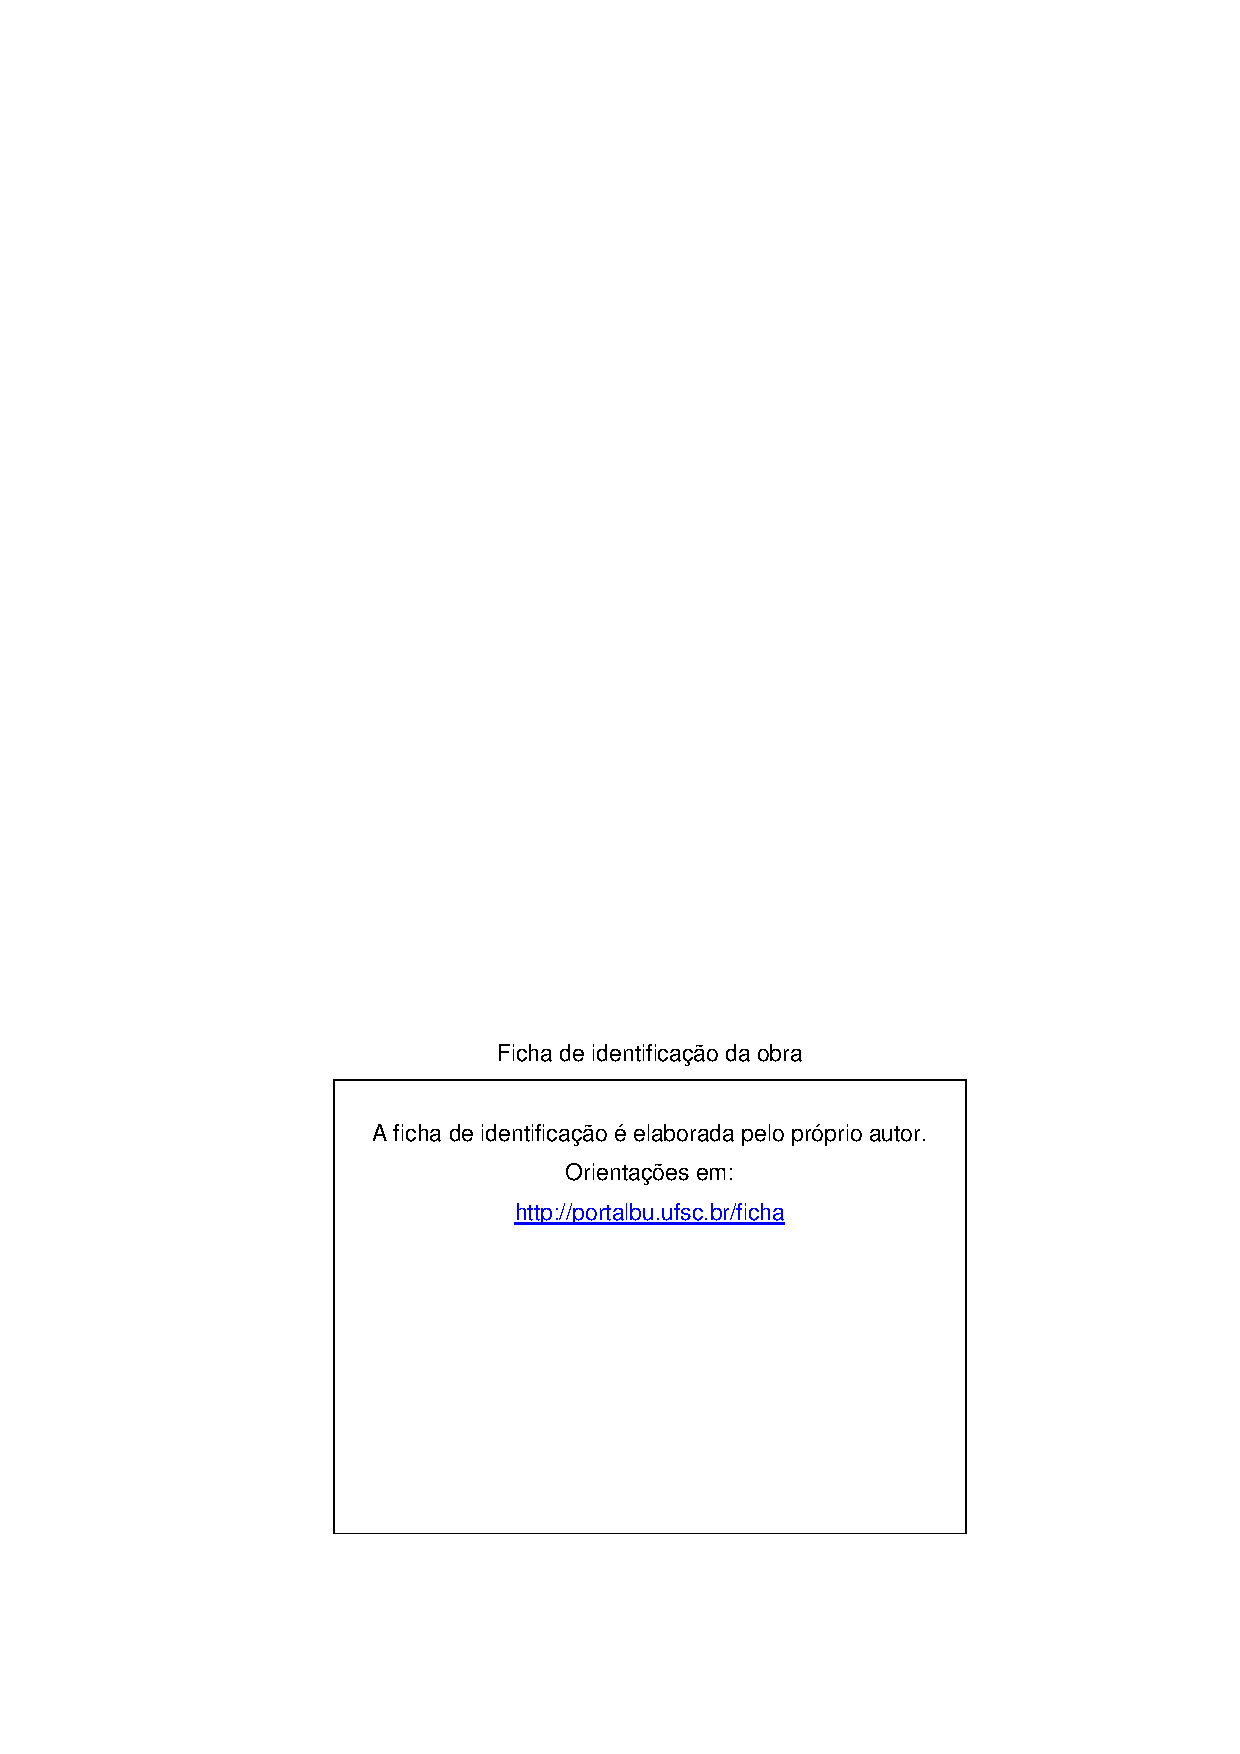
\includepdf{beforetext/Ficha_Catalografica.pdf}
\end{fichacatalografica}
% ---

% ---
% Inserir folha de aprovação
% ---
\begin{folhadeaprovacao}
	\OnehalfSpacing
	\centering
	\imprimirautor\\%
	\vspace*{10pt}		
	\textbf{\imprimirtitulo}%
	\ifnotempty{\imprimirsubtitulo}{:~\imprimirsubtitulo}\\%
	%		\vspace*{31.5pt}%3\baselineskip
	\vspace*{\baselineskip}
	%\begin{minipage}{\textwidth}
	% ~do~\imprimirprograma~do~\imprimircentro~da~\imprimirinstituicao~para~a~obtenção~do~título~de~\imprimirformacao.
	Este~\imprimirtipotrabalho~foi julgado adequado para obtenção do Título de “\imprimirformacao” e aprovado em sua forma final pelo~\imprimirprograma. \\
		\vspace*{\baselineskip}
	\imprimirlocal, \imprimirdata. \\
	\vspace*{2\baselineskip}
	\assinatura{\OnehalfSpacing\imprimircoordenador \\ \imprimircoordenadorRotulo~do Curso}
	\vspace*{2\baselineskip}
	\textbf{Banca Examinadora:} \\
	\vspace*{\baselineskip}
	\assinatura{\OnehalfSpacing\imprimirorientador \\ \imprimirorientadorRotulo}
	%\end{minipage}%
	\vspace*{\baselineskip}
	\assinatura{Prof.(a) xxxx, Dr(a).\\
	Avaliador(a) \\
	Instituição xxxx}

	\vspace*{\baselineskip}
	\assinatura{Prof.(a) xxxx, Dr(a).\\
	Avaliador(a) \\
	Instituição xxxx}


\end{folhadeaprovacao}
% ---

% ---
% Dedicatória
% ---
\begin{dedicatoria}
	\vspace*{\fill}
	\noindent
	\begin{adjustwidth*}{}{5.5cm}     
		Dedico o presente trabalho à minha mãe, que meu fazer ciência seja tão legal aos seus olhos quanto nos filmes que assistimos juntos.
		
	\end{adjustwidth*}
\end{dedicatoria}
% ---

% ---
% Agradecimentos
% ---
\begin{agradecimentos}
	Inserir os agradecimentos aos colaboradores à execução do trabalho. 
	
	Xxxxxxxxxxxxxxxxxxxxxxxxxxxxxxxxxxxxxxxxxxxxxxxxxxxxxxxxxxxxxxxxxxxxxx. 
\end{agradecimentos}
% ---

% ---
% Epígrafe
% ---
\begin{epigrafe}
	\vspace*{\fill}
	\begin{flushright}
		\textit{“Acredito que a única coisa 	 mais importante,\\
		 além da disciplina e da criatividade,\\ 
		é ter a coragem de arriscar.”\\
			— Maya Angelou
		}
	\end{flushright}
\end{epigrafe}
% ---

% ---
% RESUMOS
% ---

% resumo em português
\setlength{\absparsep}{18pt} % ajusta o espaçamento dos parágrafos do resumo
\begin{resumo}
	\SingleSpacing
Durante o mês de setembro de 2024, ocorreu sobre todo o estado de Santa Catarina, Brasil diversos fenômenos atmosféricos associados à poluição do ar, como eventos de black rain, quedas bruscas nos índices de qualidade do ar e consequentemente o agravamento de doenças respiratórias na população. Na época, a região oeste do estado não apresentava estações de qualidade do ar ativas, gerando uma lacuna de informações detalhadas sobre os impactos desses fenômenos no território. No presente trabalho é proposto estudo de caso a partir de dados meteorológicos de diferentes reanálises globais com os objetivos de: Identificar os períodos de maior presença de aerossóis na atmosfera (bem como as espécies de poluentes presentes); Investigar o padrão atmosférico que pode ter contribuído para o transporte desses poluentes até o estado de SC; E simular através do modelo de trajetória híbrida HYSPLIT o transporte e dispersão desses aerossóis levando em conta as características da atmosfera, as propriedades físico-químicas dos aerossóis identificados na primeira parte do estudo e a ocorrência de incêndios na floresta amazônica na época. Resultados preliminares indicam que a região oeste do estado foi a mais afetada, reforçando a necessidade de investigações mais detalhadas neste recorte geográfico.
	
	\textbf{Palavras-chave}: Palavra-chave 1. Palavra-chave 2. Palavra-chave 3.
\end{resumo}

% resumo em inglês
\begin{resumo}[Abstract]
	\SingleSpacing
	\begin{otherlanguage*}{english}
		During September 2024, the state of Santa Catarina, Brazil was the stage for several atmospheric phenomena associated with air pollution, such as black rain, sudden drops in air quality indexes and therefore the aggravation of respiratory diseases in the population. At the time, the western region of the state didn’t have active air quality meteorologic stations, which culminated in a lack of detailed information on the impacts of such occurrences in the territory. In the present work it is proposed a case study starting from data made available by different global reanalyses with the following goals: Identifying the periods of highest aerosol occurrence in the atmosphere (as well as the species of pollutants that were registered); Assessing the atmospheric pattern that may have contributed to the transport of these pollutants to the state of SC; And simulating with the HYSPLIT hybrid trajectory model the transport and dispersion of these aerosols taking into account the physical and chemical properties of the pollutants identified in the first part of the study and the occurrence of wildfires in the amazon forest at the time. Preliminary results indicate that the western region was the most affected, reinforcing the need for further detailed investigation in this geographic scope.
		
		
		\textbf{Keywords}: Keyword 1. Keyword 2. Keyword 3.
	\end{otherlanguage*}
\end{resumo}

%% resumo em francês 
%\begin{resumo}[Résumé]
% \begin{otherlanguage*}{french}
%    Il s'agit d'un résumé en français.
% 
%   \textbf{Mots-clés}: latex. abntex. publication de textes.
% \end{otherlanguage*}
%\end{resumo}
%
%% resumo em espanhol
%\begin{resumo}[Resumen]
% \begin{otherlanguage*}{spanish}
%   Este es el resumen en español.
%  
%   \textbf{Palabras clave}: latex. abntex. publicación de textos.
% \end{otherlanguage*}
%\end{resumo}
%% ---

{%hidelinks
	\hypersetup{hidelinks}
	% ---
	% inserir lista de ilustrações
	% ---
	%\pdfbookmark[0]{\listfigurename}{lof}
	%\listoffigures*
	%\cleardoublepage
	% ---
	
	% ---
	% inserir lista de quadros
	% ---
	%\pdfbookmark[0]{\listofquadrosname}{loq}
	%\listofquadros*
	%\cleardoublepage
	% ---
	
	% ---
	% inserir lista de tabelas
	% ---
	%\pdfbookmark[0]{\listtablename}{lot}
	%\listoftables*
	%\cleardoublepage
	% ---
	
	% ---
	% inserir lista de abreviaturas e siglas (devem ser declarados no preambulo)
	% ---
	%\imprimirlistadesiglas
	% ---
	
	% ---
	% inserir lista de símbolos (devem ser declarados no preambulo)
	% ---
	%\imprimirlistadesimbolos
	% ---
	
	% ---
	% inserir o sumario
	% ---
	\pdfbookmark[0]{\contentsname}{toc}
	\tableofcontents*
	\cleardoublepage
	
}%hidelinks
% ---
	
	% ----------------------------------------------------------
	% ELEMENTOS TEXTUAIS
	% ----------------------------------------------------------
	\textual
	
	% ----------------------------------------------------------
\chapter{Introdução}
% ----------------------------------------------------------

	Durante o fim do inverno austral em 2024 o estado de Santa Catarina, Brasil registrou fenômenos atmosféricos sem precedentes associados à qualidade do ar e poluição, tais como a queda na umidade relativa que em conjunto com altas concentrações de fumaça no ar criaram condições mais favoráveis para o agravamento de doenças respiratórias (as quais já estavam em seu pico por conta da estação do ano), conforme indicado pela \autocite{santacatarina_ima2026}.  As notas emitidas fizeram referência às quedas na qualidade do ar observadas nas quatro estações meteorológicas instaladas nas regiões central e litorânea do estado, enquanto as previsões meteorológicas oficiais indicavam uma atmosfera estável pelos próximos dias, fator que contribui fortemente para a estagnação de poluentes na atmosfera. Adicionalmente, registros de chuva preta nas cidades do estado mostram que o impacto não se limitou às áreas onde observações in situ puderam ser feitas  \autocite{epagri2024chuvapreta}.
	
	Neste contexto, pesquisas foram conduzidas com o intuito de avaliar o transporte de aerossóis em municípios de estados do Rio Grande do Sul e de São Paulo durante essa mesma época do ano, onde os autores apontaram os incêndios generalizados na floresta amazônica que estavam ocorrendo na época como fonte dos aerossóis transportados até as  localidades analisadas \autocite{forgioni2025}. No referente à Santa Catarina, a ausência de instrumentos de observação na região oeste do estado na época do ocorrido cria uma lacuna de informações sobre o real impacto desse episódio na população. Portanto, é proposto no presente trabalho um estudo de caso sobre o transporte e a dispersão dos aerossóis presentes na atmosfera da região oeste do estado de Santa Catarina a partir de registros feitos tanto com satélites quanto com dados de reanálise, que combinam dados observados com interpolações de saídas de modelos numéricos para cobrir áreas sem registro. Uma vez obtidos e tratados, esses dados servem de base para simulações computacionais que forneçam detalhes precisos sobre o transporte e a dispersão dos poluentes ao longo do tempo. A seguir estão dispostos tanto o objetivo geral quanto os objetivos específicos do trabalho. 



% ----------------------------------------------------------
\section{Objetivos}
% ----------------------------------------------------------

Nas seções abaixo estão descritos o objetivo geral e os objetivos específicos deste TCC.

% ----------------------------------------------------------
\subsection{Objetivo Geral}
% ----------------------------------------------------------

	Simular o transporte e dispersão dos poluentes presentes na região oeste de Santa Catarina durante os dias de máxima profundidade óptica de aerossóis observadas em setembro de 2024.

% ----------------------------------------------------------
\subsection{Objetivos Específicos}
% ----------------------------------------------------------

	\begin{itemize}
		\item Identificar o padrão atmosférico da época sobre a América do Sul, com ênfase nos sistemas e mecanismos que influenciaram a intensidade e duração do evento.
		\item Analisar o tipo e a concentração de aerossóis que foram registrados no estado de Santa Catarina.
		\item Gerar simulações de trajetória e dispersão no Modelo Hysplit a partir de dados de reanálise de variáveis meteorológicas e de emissão por queimadas.
	\end{itemize}
	
	
	
	% ----------------------------------------------------------
\chapter{Revisão Bibliográfica}\label{cap:desenvolvimento}
% ----------------------------------------------------------
	Neste capítulo contextualizamos os objetos de estudo utilizados no trabalho iniciando por uma revisão teórica sobre a definição e diferentes classificações de aerossóis. Em seguida apresentamos referencial teórico sobre jato de baixos níveis com ênfase no fenômeno sul-americano, detalhando seus impactos no clima do continente e critérios de identificação.
% ----------------------------------------------------------
\section{Aerossóis}
% ----------------------------------------------------------

	Define-se o conceito de aerossol por uma coleção de partículas, sólidas ou líquidas, suspensas em um gás, com dimensões que variam entre alguns micrômetros até dezenas de nanômetros. No contexto da meteorologia, se atribui o termo "aerossol" apenas às partículas suspensas, sem levar em conta o gás atmosférico \autocite{boucher2015,seinfeld2006}. Seus impactos são diversos, pois interagem de forma direta com as radiações terrestre e solar através da absorção e espalhamento das mesmas, e também indiretamente ao atuarem como núcleos de condensação de nuvens, o que atribui aos mesmos um papel importante não só no balanço de radiação do planeta, mas também no sistema hidrológico e elétrico terrestre \autocite{carslaw2022a}.  Adicionalmente, é pertinente vincular a discussão à uma perspectiva de saúde humana, uma vez que a poluição do ar é o segundo maior fator de risco para morte em escala global \autocite{stateofglobalair2025}.
	
	No que compete à classificação, existem diversas propostas para sistematizar as diferentes populações de aerossóis na atmosfera. As abordagens mais usadas se baseiam na composição química das partículas, no seu processo de formação e no seu local de origem \autocite{boucher2015}.
	

% ----------------------------------------------------------
\subsection{Processo de Formação}
% ----------------------------------------------------------
	Considera-se um aerossol primário quando o material é emitido na atmosfera com forma, composição química e tamanho relativamente definidos, não havendo necessidade de interações físico-químicas para que o mesmo atinja seu estágio final. Como exemplos temos o sea spray, proveniente do atrito entre ventos e a superfície do oceano, partículas de poeira suspensas a partir de solo exposto às intempéries, além de fuligem criada por combustão incompleta de material orgânico \autocite{boucher2015}. 
	Aerossóis secundários são formados a partir de gases já suspensos na atmosfera, denominados precursores segundo \textcite{boucher2015}, que acabam por se tornarem aerossóis através do processo de nucleação. De acordo com \textcite{seinfeld2006}, esse fenômeno é parte da mudança de fase em processos termodinâmicos e faz referência ao fato de que a alteração de estado da matéria não ocorre de forma homogênea e nem instantânea, mas sim em agrupamentos que vão aumentando ao longo do tempo. No contexto de aerossóis secundários, conforme adotado por \textcite{boucher2015}, é de interesse simplificar o termo ”nucleação” ao agrupamento das moléculas sem a presença de um núcleo ou superfícies distintas que servirão de alicerce para o processo. Exemplos de precursores de aerossóis são dióxido de enxofre (SO2), amônia (NH3), Compostos Orgânicos Voláteis (COV), Óxidos de Nitrogênio (NOx) e Sulfeto de Dimetila (DMS) \autocite{carslaw2022a}. Um esquema conceitual da emissão, interação com a atmosfera e fim do ciclo de vida de aerossóis, tanto primários quanto secundários, e sua relação de distribuição de tamanhos ao longo desses processos é apresentado na Figura \ref{fig:process}.
	
	

\begin{figure}[htb]
	\begin{center}
		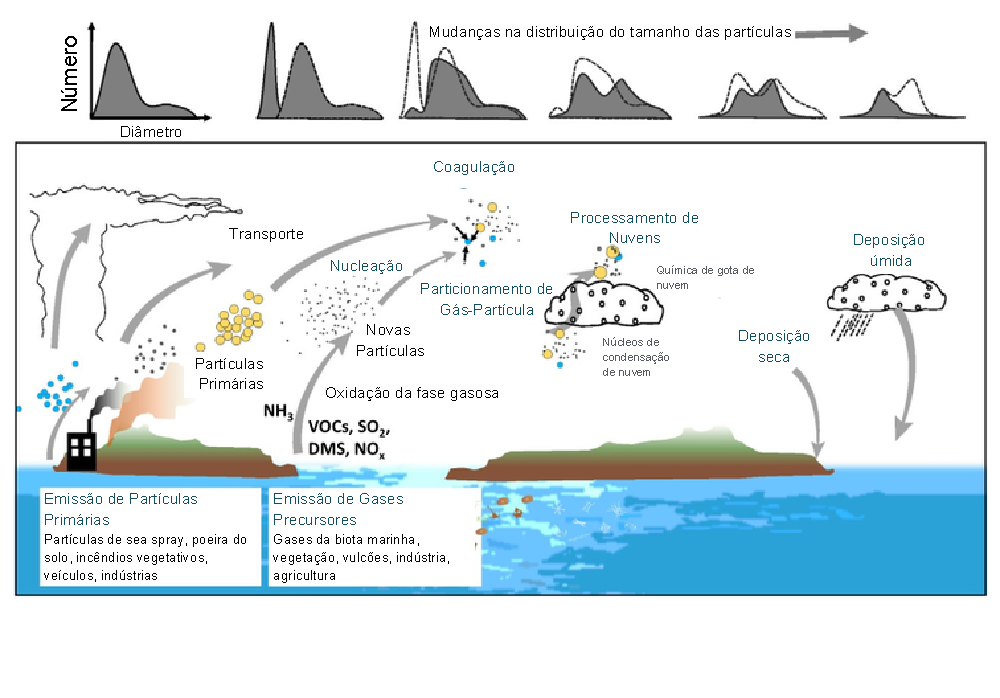
\includegraphics[trim=0cm 1.7cm 0cm 0cm, clip]{images/figura1.pdf}

	\end{center}
	\caption{Processos de transformação química e microfísica de aerossóis na atmosfera. A evolução aproximada da distribuição de tamanho das partículas é mostrada na linha superior correspondente ao processo na figura principal \autocite{carslaw2022a}.}
	\label{fig:process}
\end{figure}

\subsection{Composição Química}
		Adicionalmente, é vantajoso classificar aerossóis por sua composição química quando o intuito é entender de forma mais detalhada os impactos desses materiais na atmosfera. A partir dessa organização é possível atribuir maior ou menor grau de protagonismo em processos de absorção e espalhamento de radiação e no processo de formação de nuvens. Por exemplo, aerossóis do tipo Black Carbon\footnote{A literatura usa o termo Black Carbon fazendo alusão à alta eficiência desse aerossol em absorver radiação solar e ao aspecto escurecido de fumaça de combustão \autocite{petzold2013}.}, com sua estrutura física exemplificada na Figura \ref{fig:bc_struc}, são originais de processos incompletos de queima de material orgânico e possuem um perfil muito higroscópico, o que os torna mais propensos a agirem como Núcleos de Condensação de Nuvens. Aerossóis Inorgânicos também são higroscópicos, porém contribuem pouco para o balanço radiativo do planeta \autocite{boucher2015}.
	\begin{figure}[htb]
		\begin{center}
			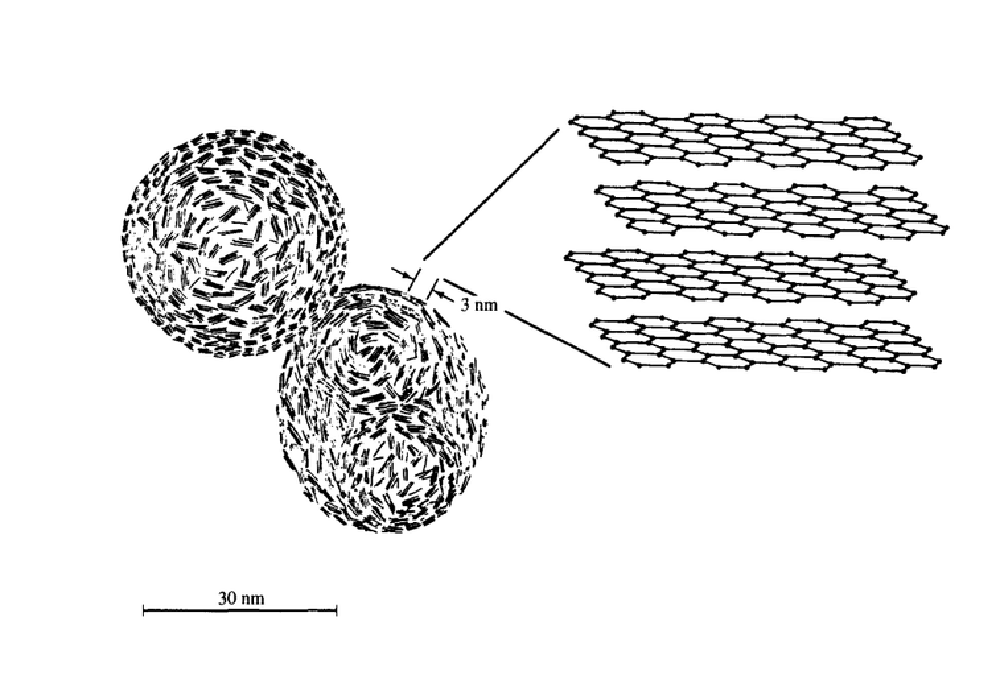
\includegraphics{images/figura2.pdf}
		\end{center}
		\caption{Esquema microestrutural de uma partícula de fuligem \autocite{seinfeld2006}}
		\label{fig:bc_struc}
	\end{figure}

\subsection{Distribuição Espacial e Temporal}
	Outra abordagem conveniente para sistematizar aerossóis se dá pelo local onde são produzidos. \textcite{boucher2015} faz distinção entre fontes naturais e antropogênicas. No que diz respeito às fontes naturais, temos oceanos, desertos, erupções vulcânicas e vegetação como fontes emissoras. Quanto às antropogênicas, leva-se em conta a ação humana na produção de aerossóis, como a queima de combustíveis fósseis e biocombustíveis, atividades tanto industriais como domésticas, além de queimadas de vegetação oriundas de ação humana. 
	
	\begin{figure}[htb]
		\begin{center}
			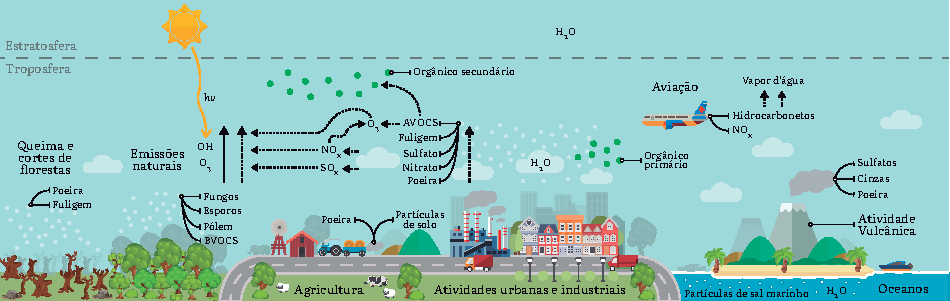
\includegraphics{images/figura3.pdf}
		\end{center}
		\caption{Principais fontes primárias e secundárias de aerossol e seu processamento na atmosfera a partir da interação entre as diversas fontes e também com a radiação solar \autocite{nascimento2021}.}
		\label{fig:nasc}
	\end{figure}

	
	Além de fontes, \textcite{boucher2015} também define o conceito de sumidouro de aerossóis, responsáveis pela deposição dessas partículas. As duas formas principais de finalizar o ciclo de vida de um aerossol são a deposição seca, que ocorre quando a partícula entra em contato com a superfície do planeta e a deposição úmida, quando a mesma é usada como núcleo de condensação para precipitação. A Figura \ref{fig:nasc} esquematiza as fontes de aerossol no sistema terrestre e suas interações com a atmosfera. 
	Por último, o que define o tempo de vida de um grupo de aerossóis na atmosfera além dos locais de gênese e deposição, é a forma com que ambos interagem com o mecanismo de transporte responsável por deslocar essas partículas de um ponto a outro.

\subsection{Distribuição de Tamanho de Partículas e Propriedades Ópticas}

	Para estudos de qualidade do ar, é comum que a nomenclatura mude de aerossóis para termos como poluentes e material particulado, com esse último englobando principalmente partículas suspensas no ar com até 1, 2.5 e 10 micrômetros em diâmetro, conforme indicado na Figura \ref{fig:uepa}. A partir dessas classificações são elaboradas legislações que visam estabelecer limites para a quantidade de materiais particulados que podem estar presentes em um local com riscos mínimos à saúde humana \autocite{usepa2019}.
	
	\begin{figure}[htb]
		\begin{center}
			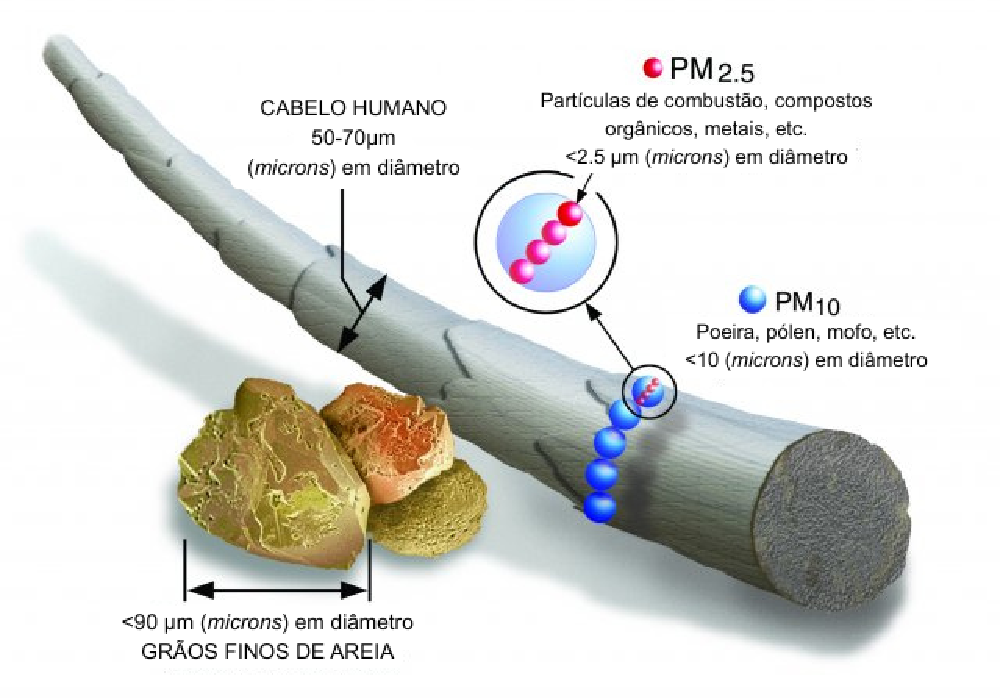
\includegraphics{images/figura4.pdf}
		\end{center}
		\caption{Figura 4: Esquema de comparação de tamanhos de MP10 e MP2.5 \autocite{usepa2019}.}
		\label{fig:uepa}
	\end{figure}  
	  
	Outra forma comum de analisar dados dessa natureza é através da profundidade óptica estimada através de satélites, onde o ponto de grade diz respeito à quantidade da partícula em questão presente em toda aquela coluna de ar, dessa forma, não é possível discretizar a concentração em níveis de altura \autocite{boucher2015}. Para os estudos de profundidade óptica e outras análises de sensoriamento, a Figura \ref{fig:distribuicao_classica} apresenta a distribuição de tamanho com mais detalhe tanto para aerossóis primários quanto secundários.
	
	\begin{figure}[htb]
	\begin{center}
		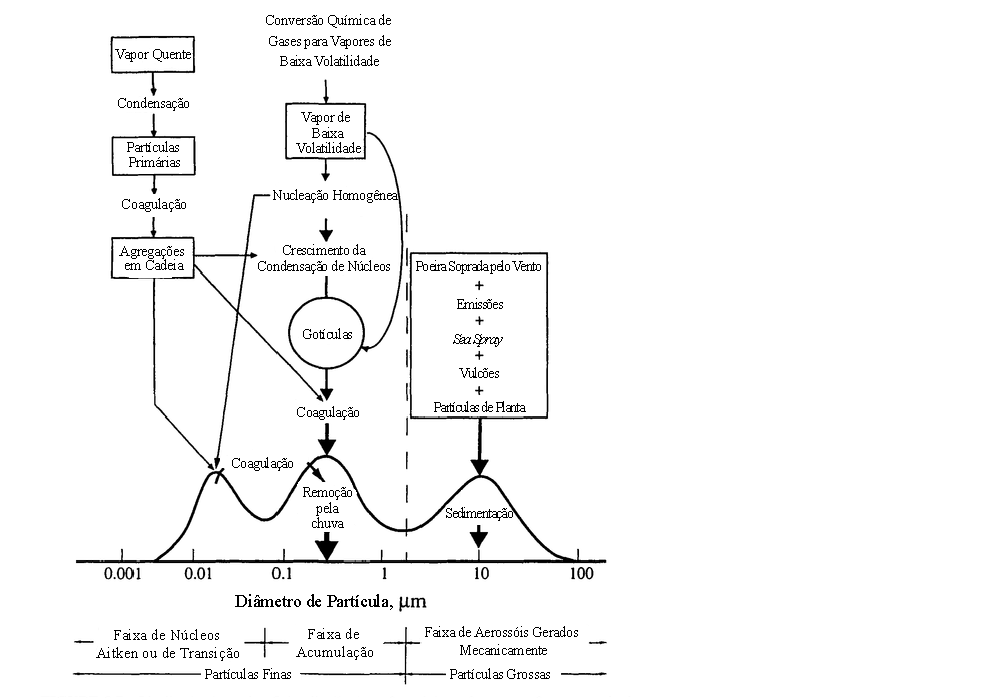
\includegraphics[trim=0cm 0cm 5cm 0cm, clip]{images/figura5.pdf}
	\end{center}
	\caption{Esquema idealizado da distribuição de área de superfície de partícula de um aerossol atmosférico, adaptado de \textcite{whitby1976}. Os principais modos, fontes e formação/remoção de partículas estão indicados.}
	\label{fig:distribuicao_classica}
	\end{figure}
	
	
	
\section{Jato de Baixos Níveis}
	Segundo \textcite{lin2007}, o Jato de Baixos Níveis (JBN) é um fenômeno de mesoescala, com distribuição horizontal na escala de milhares de quilômetros e temporal de alguns dias, composto de corrente de ar que se desloca com altas velocidades próximo à superfície terrestre, entre 2 e 3 km de altura. Sua importância para a meteorologia se dá por ser um mecanismo de transporte de temperatura e umidade, além de possuir dinâmicas muito específicas influenciadas pela orografia e ter uma relação intrínseca com a ocorrência de outros fenômenos atmosféricos de mesoescala. Os exemplos mais significativos são o JBN das grandes planícies nos Estados Unidos e o JBN da América do Sul, mas também existem registros da ocorrência desse mesmo fenômeno em diversos outros lugares. Em primeira instância, a caracterização do JBN se deu pelo Critério de \textcite{bonner1968}, onde o sistema se configura através de:
	\begin{itemize}
		\item Ventos meridionais iguais ou superiores a 12 $ms^{-1}$ no nível de 850 hPa;
		\item Cisalhamento vertical do vento de no mínimo 6 $ms^{-1}$ entre os níveis de 700 e 850 hPa;
		\item Componente meridional do vento maior em extensão que a componente zonal; \autocite{marengo2009}. 
	\end{itemize}
	
\section{Jato de Baixos Níveis da América do Sul}
	Ainda de acordo com \autocite{marengo2009}, o Jato de Baixos Níveis da América do Sul, comumente referido por South American Low-Level Jet (SALLJ), é um fenômeno recorrente na América do Sul caracterizado por um fluxo intenso de ventos a leste da cordilheira dos Andes, conforme indicado na Figura \ref{fig:sallj}.  Os estudos com relação ao tópico iniciaram na década de 1980 e encontraram avanços significativos com as tecnologias de reanálise de dados e modelagem numérica da atmosfera, sendo possível identificar que o mesmo nem sempre ocorre de forma homogênea ou contínua ao longo da América do Sul \autocite{jones2019}.  Por conta da floresta amazônica e sua alta injeção de umidade na atmosfera, \autocite{herdies2002} aponta o SALLJ como parte de um mecanismo bimodal de redistribuição tanto de umidade quanto de calor partindo da região norte da AS em direção às regiões centrais e sul do Brasil, atuando em conjunto com a Zona de Convergência do Atlântico Sul (ZCAS) ao longo da estação chuvosa (meses de verão), o que favorece a ocorrência de eventos de precipitação intensos com grande impacto nas regiões sul e sudeste do país. Adicionalmente, o transporte de umidade contribui em outros momentos na formação e manutenção de Complexos Convectivos de Mesoescala e sistemas frontais comuns na região \autocite{reboita2015}. 
	
	Quanto aos pormenores de sua classificação, \autocite{montini2019} argumenta que o critério previamente utilizado, por ter sido elaborado com valores empíricos obtidos nas Grandes Planícies da América do Norte, apresenta vieses na identificação de eventos de ocorrência do SALLJ, uma vez que o perfil de ventos na América do Sul apresenta uma variabilidade sazonal muito distinta quando comparada com os dados obtidos por \autocite{bonner1968} e adaptados por \autocite{marengo2009}. Em sua análise do fenômeno por uma perspectiva climatológica, a autora atualiza o critério de Bonner/Marengo se baseando em  percentis climatológicos do perfil de ventos e fluxos de umidade elaborados com reanálises e sondagens. A partir disso, os critérios são:
	
	\begin{itemize}
		\item Velocidade do vento em 850 hPa excedendo o percentil 75\% para a época do ano em questão;
		\item Cisalhamento vertical do vento entre 850 e 700 hPa também excedendo o percentil citado anteriormente;
		\item Direção do vento em 850 hPa entre 292.5° e 45°; \autocite{montini2019}.
	\end{itemize}
	
	\autocite{montini2019} também conclui que o SAALJ ocorre em quantidade muito maior do que o considerado pelos antigos parâmetros ao longo do ano, com as máximas de velocidade do vento permanecendo nos meses de inverno.
	
	\begin{figure}[htb]
		\begin{center}
			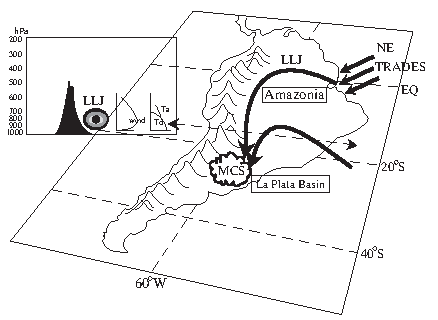
\includegraphics{images/figura6.pdf}
		\end{center}
		\caption{Modelo conceitual descrevendo o JBN da América do Sul a leste dos Andes \autocite{marengo2004}.}
		\label{fig:sallj}
	\end{figure}
	
	
	Outro resultado interessante proveniente dos avanços da tecnologia na área de sensoriamento remoto dentro do estudo dos Jatos é a possibilidade de replicar o conceito de mecanismo de transporte para outros componentes da atmosfera, como é o caso do transporte de aerossóis através de rios atmosféricos \autocite{chakraborty2022}. Mais especificamente, \autocite{forgioni2025} utilizam do SALLJ para caracterizar o transporte em longa distância de aerossóis provenientes de queimadas na Amazônia para os estados de São Paulo e Rio Grande do Sul em setembro de 2024. 

\section{Bloqueios Atmosféricos}
\label{sec:bloqueio}
	
	De acordo com \textcite{holton2012introduction}, o escoamento de ar em latitudes médias possui um sentido predominantemente zonal e de oeste em médios e altos níveis, como resultado do equilíbrio geostrófico, entre as forças defletora e Coriolis e a força Gradiente de Pressão. Essa característica da atmosfera é responsável pelo deslocamento espacial de diferentes fenômenos atmosféricos ao longo do tempo. Porém, num contexto de bloqueio atmosférico, a componente meridional do escoamento é alongada por conta da combinação de centros de alta e baixa pressão estacionários (de no mínimo seis dias). Como consequência, a intensidade, extensão e duração desses sistemas sinóticos são alteradas drasticamente \autocite{ambrizzi2009bloqueios}.
	
	
	No Hemisfério Sul, em especial, \textcite{mendes2008blocking} destaca como impacto de Bloqueios no Sul do Brasil a alteração nos regimes precipitação, como o impedimento do avanço de sistemas frontais, os quais influenciam na remoção de aerossóis da atmosfera através do processo de deposição úmida: os aerossóis são utilizados como núcleos de condensação para nuvens (\textit{in-cloud scavenging}) e são arrastados para a superfície através dos fluxos de ar provenientes da precipitação (\textit{below-cloud scavenging}) \autocite{boucher2015}.   
	Como formas de identificação, \textcite{rex1950effect} foi o primeiro a mapear as características comuns aos padrões de bloqueios, com \textcite{vanloon1956blocking} refinando a pesquisa para o Hemisfério Sul:
	\begin{itemize}
		\item O deslocamento do sistema de bloqueio, dados pelo movimento do centro de alta, não deve exceder 25° de longitude em 45°S durante todo seu período;
		\item O centro do anticiclone de bloqueio deve estar pelo menos 10° de latitude mais ao sul do cinturão de altas pressões subtropicais;
		\item O bloqueio deve durar pelo menos seis dias.
	\end{itemize}
	
 
	
	As diferentes possibilidades de configuração de circulação que podem ser encontradas em bloqueios atmosféricos estão representadas na Figura \ref{fig:block}.
	\begin{figure}[htb]
		\begin{center}
			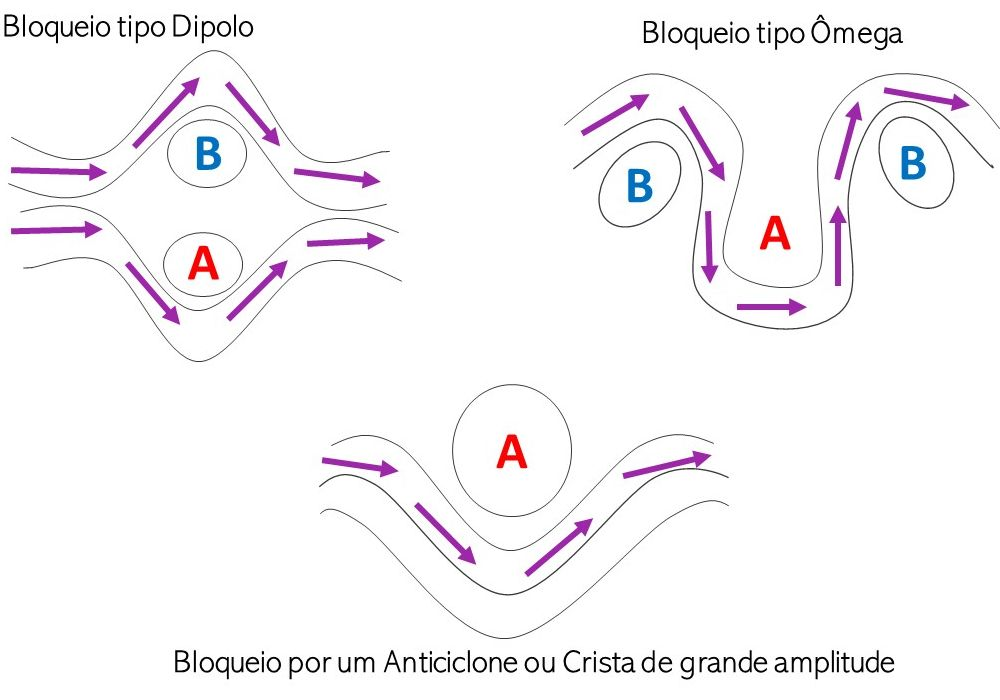
\includegraphics[width=\textwidth]{images/tiposdebloqueio.jpg}
		\end{center}
		\caption{Os três tipos de padrões de bloqueios e as alterações sofridas pelos Jatos de Altos Níveis (setas roxas). \autocite{bueno2019bloqueios}.}
		\label{fig:block}
	\end{figure}
	% ----------------------------------------------------------
\chapter{Metodologia}
% ----------------------------------------------------------
	Nesta seção do trabalho, definimos a área geográfica do estudo, assim como os conjuntos de dados levantados para as análises que servirão de base para as simulações de trajetória e dispersão dos poluentes, bem como detalhamentos sobre a obtenção das mesmas.
	
\section{Área de Estudo}
\subsection{Santa Catarina}  
	O estado de Santa Catarina, situado na região sul do Brasil, entre as latitudes de 25º57'41" e 29º23'55", e longitudes 48º19'37" e 53º50'00" possui uma paisagem muito diversificada, com uma faixa litorânea sobre o Oceano Atlântico, o estado também conta com regiões de Serra, Planaltos e Planícies que se estendem até a divisa com a Argentina. Sua mesorregião oeste, conforme indicado na Figura 7 como foco do estudo, situada entre os Planaltos dos rios Uruguai e Iguaçu, possui aproximadamente 23.710 km2 e possui temperaturas médias entre 13 e 16 °C e valor médio de precipitação entre 420 e 480 mm para o período de inverno do hemisfério sul, compreendido entre 21 de junho e 22 de setembro \autocite{santacatarina_seplan2016}.
	
	De acordo com o Atlas Climático proposto por \autocite{oliveira2024}, as mesorregiões Oeste/Extremo Oeste não possuem estações seca e úmida bem definidas, e seus menores acumulados de precipitação se encontram ao longo do inverno, fenômeno atrelado à presença de bloqueios atmosféricos causados por sistemas de alta pressão que impedem a passagem de sistemas frontais. Quanto aos maiores acumulados de precipitação, o autor atribui a influência do SAALJ no transporte de umidade proveniente da Amazônia para a região sul do continente, que contribui com o aumento de eventos convectivos e de Sistemas Convectivos de Mesoescala na região.
	
\begin{figure}[htb]
	\begin{center}
		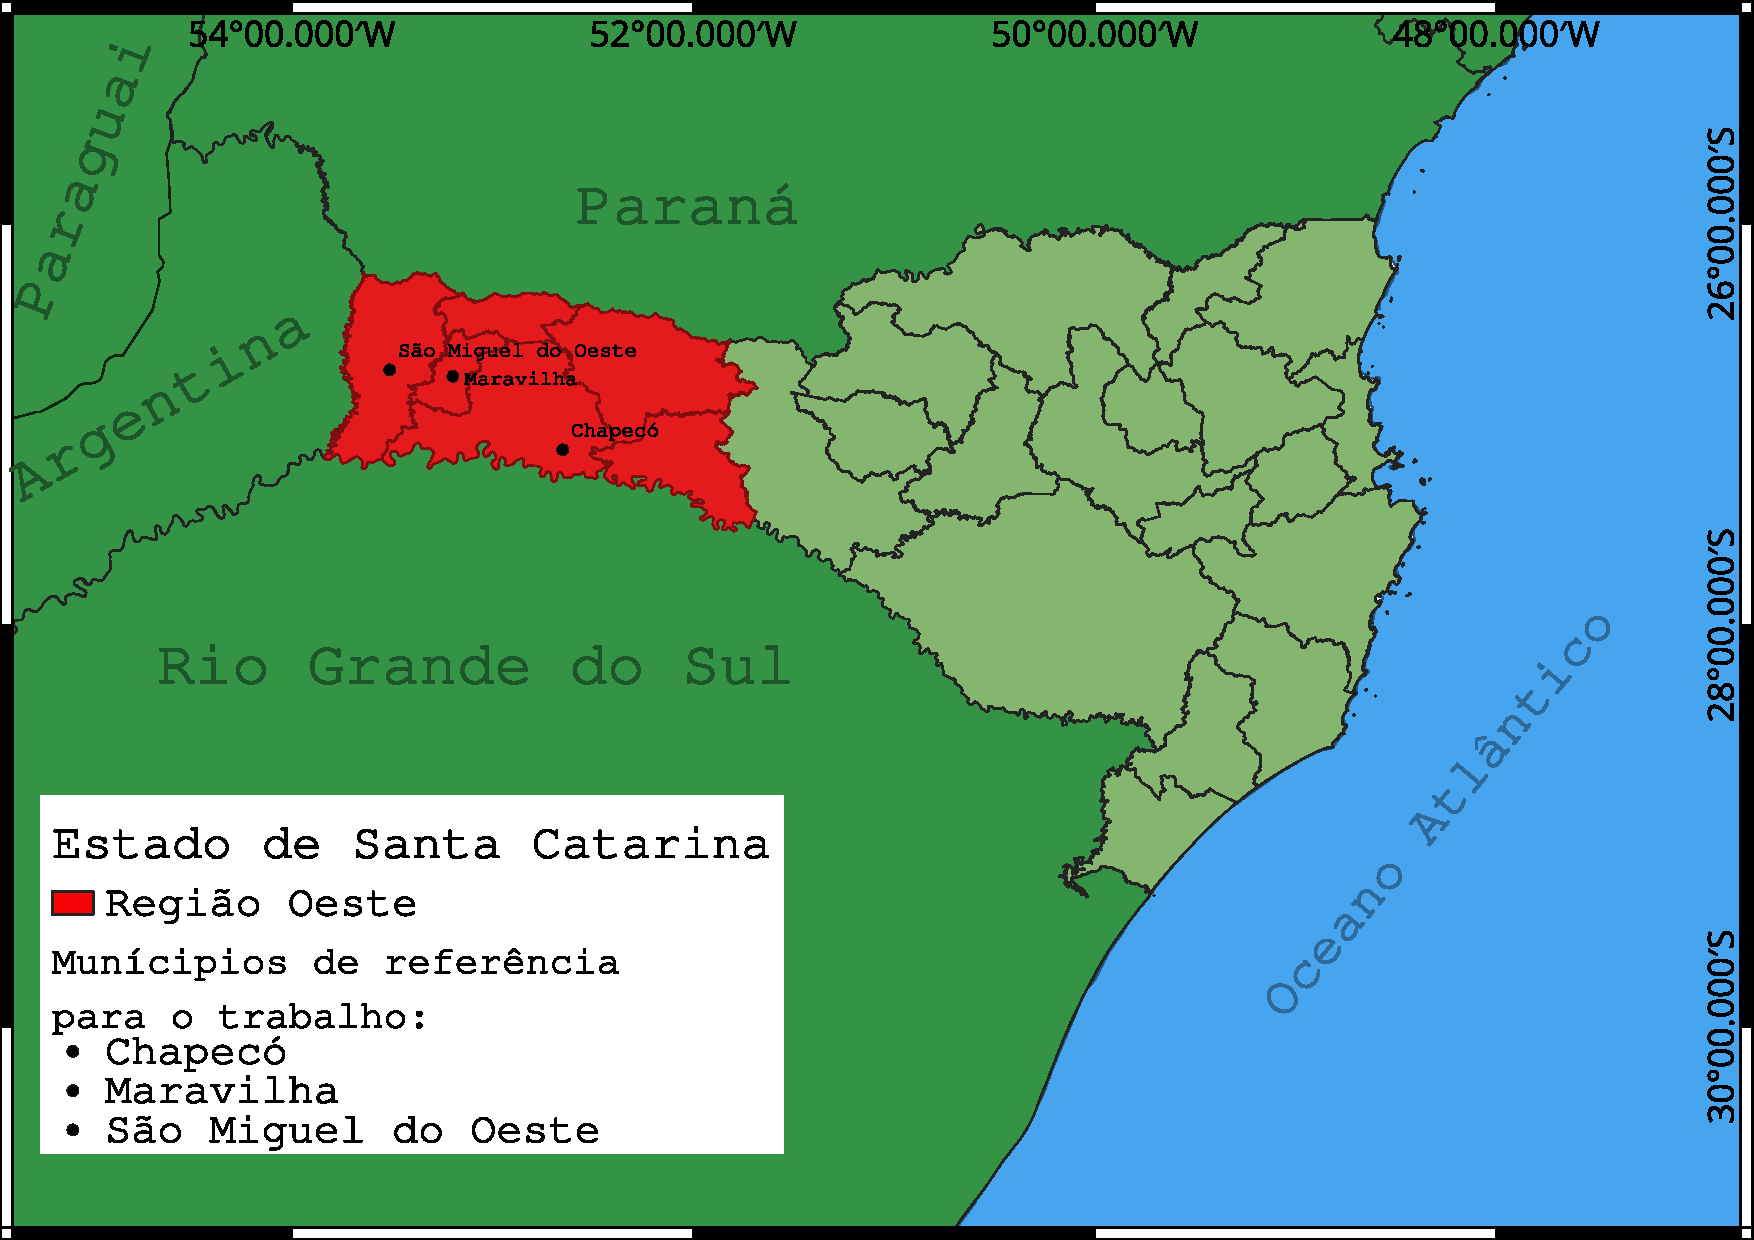
\includegraphics[width=\textwidth]{images/figura7.pdf}
	\end{center}
	\caption{Mapa do estado de Santa Catarina com destaque para a região oeste. Elaboração do autor com dados do IBGE.}
\end{figure}

\section{Dados Utilizados}
\subsection{Reanálise \textit{Copernicus Atmosphere Monitoring Service} (CAMS) EAC4}

	Produto também disponibilizado pelo ECMWF (European Centre for Medium-Range Weather Forecasts), a reanálise CAMS (Copernicus Atmosphere Monitoring Service) é composta por uma assimilação de dados referentes à composição da atmosfera, com foco na identificação de aerossóis e espécies químicas. O conjunto conta com dados em escala de 3 horas, cobrindo toda a superfície terrestre com resolução de 0.75° e duas diferentes formas de espacializar o dado verticalmente (por níveis de pressão e 60 níveis próprios do produto). As variáveis disponíveis possuem alguma semelhança com as da reanálise ERA5 (vento e temperatura, por exemplo) mas se distingue pelo detalhamento nas espécies químicas e quantificações de aerossóis \autocite{inness2019}. Para o presente trabalho, serão analisadas as seguintes variáveis:
	\begin{itemize}
		\item Profundidade Óptica de Black Carbon a 550 nm (Black Carbon AOD) (Adimensional)
		\item Material Particulado com até 1 nm de diâmetro (PM$_{1}$) ($kgm^{3}$)
		
	\end{itemize}

\subsection{Reanálise ERA5}

	Criada e mantida pelo European Centre for Medium-Range Weather Forecasts (ECMWF), a reanálise ERA-5 conta com diversas variáveis meteorológicas agrupadas em uma grade espacial de 31km, distribuídas em 137 níveis distintos de pressão com registros desde o ano de 1940. Para o presente trabalho foram coletados dados entre as datas 11/09/2024 e 13/09/2024, com resolução horária nos seguintes conjuntos de reanálise \autocite{hersbach2020}:
	
	\begin{itemize}
		\item \textit{ERA5 hourly data on pressure levels from 1940 to present}
		\begin{itemize}
			\item Componente zonal do vento ($ms^{-1}$)
			\item Componente meridional do vento ($ms^{-1}$)
			\item Velocidade vertical do vento($Pas^{-1}$)
			\item Umidade relativa (\%)
			\item Geopotencial ($m^{2}s^{-1}$)
			\item Temperatura (K)
		\end{itemize}
		\item \textit{ERA5 hourly data on single levels from 1940 to present}
		\begin{itemize}
			\item Temperatura a 2 metros do solo (K)
			\item Pressão à superfície (Pa)
			\item Precipitação total (m)
			\item Geopotencial ($m^{2}s^{-1}$)
		\end{itemize}
	\end{itemize}
	
\subsection{Satélite Goes-16}
	Operado pela \textit{National Oceanic and Atmospheric Administration} (NOAA) e pela \textit{National Aeronautics and Space Administration} (NASA), o satélite GOES-16 monitora os continentes americanos norte e sul, bem como oceanos que os delimitam através de uma órbita geoestacionária que o posiciona de forma constante com relação à essa face específica do planeta terrestre. Dentre suas diferentes aplicações, o satélite conta com um sensor multiespectral de alta resolução espacial e temporal que consegue captar dados em 16 bandas diferentes do espectro eletromagnético \autocite{goodman2019goes}. 
	
	 
	Em especial, o canal 13 (comumente referenciado como Infravermelho Limpo, centrado em 10,3 $\mu m$) se destaca como ferramenta essencial para análises de condições meteorológicas por permitir a identificação do topo de nuvens independente do ciclo diurno, com isso, torna-se possível a demarcação de sistemas sinóticos \autocite{schmit2017closer}.
	
\subsection{\textit{CAMS Global Fire Assimilation System} (GFAS)}
\label{subsec:cams-gfas}

	Partindo das observações de Potência Radiativa do Fogo obtidas feitas por satélites, a reanálise GFAS disponibiliza informações sobre a localização, intensidade relativa e emissões estimadas de queima de biomassa e incêndios de vegetação. O resultado é uma reanálise com 0.1° de resolução espacial e resolução temporal de um dia \autocite{kaiser2012}. Para o presente trabalho foram utilizadas as seguintes variáveis:
	\begin{itemize}
		\item Altura de Injeção ($m$)
		\item Base da Pluma acima da Superfície ($m$)
		\item Fluxo de queima de Black Carbon ($kgm^{-2}s^{-1}$)
		\item Fluxo de queima de Material Particulado Total ($kgm^{-2}s^{-1}$)
		\item Fluxo de queima de Dióxido de Carbono ($kgm^{-2}s^{-1}$)
	
	\end{itemize}
\subsection{Modelo HYSPLIT}
	O Hybrid Single-Particle Lagrangian Integrated Trajectory  (HYSPLIT) é um modelo lagrangiano de trajetórias criado pelo Air Source Laboratory, administrado pela National Oceanic and Atmospheric Administration (NOAA) dos Estados Unidos, com o qual é possível calcular transporte e dispersão atmosféricos. Suas aplicações variam entre o rastreio e previsão da liberação de material radioativo, poeira transportada pelo vento e fumaça liberada por queimadas. Apesar do nome, o modelo acaba por misturar as abordagens lagrangeanas e eulerianas no seu método de cálculo: a primeira é utilizada na descrição da trajetória das partículas/massas de ar ao longo da simulação, enquanto o referencial euleriano é empregado para calcular as concentrações do poluente em uma grade fixa.
	
	O fluxo de uso do modelo consiste no pré-processamento de dados meteorológicos que servirão de base para a execução das simulações, sendo possível simular trajetórias tanto avançando quanto retrocedendo no tempo (comumente referidas como forward e backward trajectories, respectivamente). Também é possível executar simulações de transporte, dispersão e deposição de poluentes atmosféricos alimentando o modelo com informações sobre as propriedades físico-químicas e taxas de emissão do aerossol em questão \autocite{stein2015}.
	
\subsection{Procedimentos}
	\subsubsection{Delimitação Espacial e Temporal}
	Como primeiro passo de execução do trabalho, foram avaliados dados da reanálise ERA5 em conjunto com imagens do satélite GOES-16 afim de estabelecer o padrão sinótico do evento. Em seguida, a reanálise CAMS foi averiguada com foco nas variáveis de profundidade óptica (AOD), buscando os períodos e pontos de máxima ao longo do estado de Santa Catarina para definir as coordenadas e datas de simulação no modelo HYSPLIT.
	
	\subsubsection{Análise Sinótica}
	Com o objetivo de identificar os padrões meteorológicos que contribuíram para a intensidade do fenômeno de transporte dos aerossóis, bem como sua duração anômala sobre o estado de Santa Catarina, foram utilizados dados do modelo ERA-5 em conjunto com imagens do satélite Goes-16 no canal 13 em intervalos de seis horas, afim de estabelecer o padrão sinótico da época. 

	\subsubsection{Trajetórias}
	
	Após produzir os mapas de profundidades ópticas, a reanálise ERA 5 foi utilizada como fonte dos dados meteorólogicos no modelo HYSPLIT. Primeiro, para as simulações de trajetória, foi necessário agrupar os dados de superfície com os dados de níveis de pressão através da ferramenta CDO \autocite{INPE2016mtc}. Em seguida, o arquivo no formato \textit{grib} foi convertido para o formato \textit{ARL}, nativo do modelo HYSPLIT.
	
	Utilizando os resultados provenientes das análises do modelo CAMS e os registros midiáticos fornecidos por \textcite{epagri2024chuvapreta}, foram definidos três municípios como pontos de referência para as trajetórias reversas das parcelas de ar: Chapecó, Maravilha e São Miguel do Oeste. Como o intuito é analisar o movimento das parcelas em função do SAALJ, foram utilizados scripts computacionais na linguagem \textit{Python} para estimar as alturas acima do nível do solo equivalentes aos níveis de pressão de 750, 800 e 850 hPa para cada um dos pontos. Para tal, os dados de geopotencial obtidos na reanálise foram convertidos para metros acima do nível do solo ($m agl$) da seguinte maneira, de acordo com \textcite{holton2012introduction}:
	\begin{equation}
		Z_{m agl} = \frac{\Phi(p)}{g} - z_{elevação}.
	\end{equation}
	
	Onde $g = 9{,}80665 \text{ms}^{2}$, $\Phi(p)$ é a altura geopotencial da camada de pressão desejada e $z_{elevação}$ é a altura média dos municípios acima do nível do mar. Os respectivos valores inseridos na rodada do modelo se encontram dispostos na Tabela \ref{table:Tabela 1}. A data selecionada para o fim da trajetória foi 13 de setembro de 2024 e a simulação teve duração total de -72h.
	

	
	\begin{table}
		\begin{center}
			\begin{tabular}{ ccc } 
				\hline
				Município & Lat Lon (°) & Níveis de altura (m-agl) \\
				\hline
				\multirow{3}{4em}{Chapecó} &  & 1850.04 \\ 
				& -27.0   -52.7 & 1305.15 \\ 
				&  & 786.94 \\ 
				\hline
								\multirow{3}{4em}{Maravilha} &  & 1976.17 \\ 
				& -26.77   -52.21 & 1432.56 \\ 
				&  & 915.06 \\ 
				\hline
								\multirow{3}{4em}{São Miguel do Oeste} &  & 1850.04 \\ 
				& -26.72   -53.51 & 1305.15 \\ 
				&  & 786.94 \\ 
				\hline
			\end{tabular}
		\end{center}
		\caption{Dados de entrada para as rodadas de trajetória reversa no modelo HYSPLIT.}
		\label{table:Tabela 1}
	\end{table}
	
	\subsubsection{Dispersão}
	Para a simulação de dispersão, foi necessário definir pontos de emissão de aerossóis provenientes de queimadas, que foram obtidos através da reanálise GFAS. Foi aplicada uma conversão nas variáveis de fluxo de emissão dos poluentes ($kgm^{-2}s^{-1}$), com o intuito de obter um valor para a taxa de emissão ($kgs^{-1}$) através da seguinte equação:
	
	\begin{equation}
		E = F * A
	\end{equation}
	
	Para a obtenção da área necessária para o cálculo, foi empregado um algoritmo computacional na linguagem \textit{Python} onde o gradeamento da reanálise é convertido da unidade de graus para $m^{2}$. Após essa conversão, foram selecionados os cinco maiores pontos de emissão de cada dia dentro da área horizontal de ocorrência do JBN definida a partir dos dados do ERA5. Neste caso, a dispersão será no sentido \textit{forward}, para que seja possível analisar quais plumas foram melhor transportadas para as regiões de interesse, além da concentração das mesmas.
	
	Para cada um dos dias compreendidos dentro da simulação, foram selecionados os cinco maiores pontos de emissão com altura de injeção da pluma mais próxima do nível de 800 hPa. Os dados de emissão implementados no modelo estão descritos na Tabela \ref{table:dados_focos}.
	
	
	\begin{table}[htbp]
		\centering
		\vspace{8pt}
		\small
		\begin{tabular}{ccccccrcc}
			\toprule
			\textbf{Data} & \textbf{Lat ($^\circ$)} & \textbf{Lon ($^\circ$)} & \textbf{Alt} (\unit{\meter}) & \textbf{Taxa} (\unit{\per\hour}) & \textbf{Área} (\unit{\meter\squared}) & \textbf{Calor} (\unit{\watt}) \\
			\midrule
			  & -18.550 & -57.750 & 1425.6 & 32\,250.50 & 117\,219\,411.3 & 2\,326\,214\,656.0 \\
			\multirow{3}{*}{2024-09-09} & -22.750 & -53.650 & 1896.3 & 31\,279.33 & 114\,023\,802.7 & 1\,381\,107\,840.0 \\
			  & -11.050 & -54.950 & 1433.3 & 25\,135.51 & 121\,350\,810.5 & 803\,256\,448.0 \\
			 & -9.350  & -55.050 & 1747.9 & 25\,031.70 & 122\,000\,433.6 & 799\,939\,136.0 \\
			 & -18.550 & -57.650 & 1564.9 & 19\,741.50 & 117\,219\,411.3 & 1\,423\,945\,856.0 \\
			\midrule
			 & -22.750 & -53.650 & 1577.3 & 23\,411.63 & 114\,023\,802.7 & 1\,033\,717\,568.0 \\
			\multirow{3}{*}{2024-09-10} & -22.750 & -53.550 & 1598.6 & 18\,932.48 & 114\,023\,802.7 & 605\,025\,920.0 \\
			 & -11.050 & -54.950 & 1433.3 & 14\,379.62 & 121\,350\,810.5 & 459\,530\,176.0 \\
			 & -15.850 & -63.850 & 1942.9 & 12\,999.00 & 118\,942\,208.0 & 415\,409\,600.0 \\
			 & -15.550 & -55.550 & 1193.9 & 9\,496.09  & 119\,117\,392.9 & 684\,949\,184.0 \\
			\midrule
			 & -10.850 & -53.050 & 1969.4 & 53\,027.97 & 121\,432\,793.1 & 1\,694\,617\,216.0 \\
			\multirow{3}{*}{2024-09-11} & -15.050 & -60.350 & 1109.1 & 25\,441.96 & 119\,402\,108.3 & 1\,835\,117\,568.0 \\
			 & -15.950 & -57.650 & 1866.7 & 18\,326.35 & 118\,883\,088.2 & 1\,321\,871\,872.0 \\
			 & -15.550 & -62.550 & 1781.5 & 12\,427.81 & 119\,117\,392.9 & 397\,156\,128.0 \\
			 & -15.950 & -57.550 & 1948.4 & 9\,241.93  & 118\,883\,088.2 & 666\,616\,128.0 \\
			\midrule
			 & -15.950 & -57.650 & 1769.9 & 22\,138.54 & 118\,883\,088.2 & 1\,596\,843\,264.0 \\
			\multirow{3}{*}{2024-09-12} & -14.750 & -65.250 & 1700.0 & 17\,709.22 & 119\,568\,574.3 & 565\,934\,272.0 \\
			 & -10.850 & -53.050 & 1969.4 & 14\,855.68 & 121\,432\,793.1 & 474\,743\,424.0 \\
			 & -11.950 & -52.950 & 1281.8 & 12\,537.89 & 120\,963\,605.8 & 400\,673\,920.0 \\
			 & -19.550 & -58.750 & 1850.0 & 10\,840.64 & 116\,515\,070.5 & 781\,930\,688.0 \\
			\bottomrule
		\end{tabular}
		\caption{Registros diários de focos, localização e taxa de emissão de calor.}
		\label{table:dados_focos}
	\end{table}
	
	Além dos dados meteorológicos e de emissões, foi necessário implementar propriedades físico-químicas para cada uma das categorias de aerossol analisadas no trabalho. Mediante a disponibilidade dos dados de emissão do GFAS, o presente trabalho gerou simulações para aerossóis do tipo \textit{Black Carbon} e $PM_{2.5}$, cujas parametrizações estão dispostas na Tabela \ref{table:fsc_qmc}.
	
	\begin{table}[htbp]
		\centering
		\begin{tabular}{llccc}
			\toprule
			\textbf{Parâmetro no \texttt{CONTROL}}  & \textbf{Valor ($\text{PM}_{2.5}$)} & \textbf{Valor (BC)} & \textbf{Unidade} \\
			\midrule
			Identificador do Poluente  & \texttt{PM25} & \texttt{BC} & -- \\
			Diâmetro da Partícula  ($d_p$) & 0.5 & 0.15 & $\mu\text{m}$ \\
			Densidade da Partícula  ($\rho$) & 1.5 & 1.0 & $\text{g/cm}^3$ \\
			Fator de Forma  ($\gamma$) & 1.0 & 1.0 & -- \\
			Velocidade de Deposição Seca  ($V_d$) & 0.0 & 0.0 & $\text{m/s}$ \\
			Constante de Henry  ($H$) & $1.0 \times 10^{4}$ & $1.0 \times 10^{-5}$ & $\text{M/atm}$ \\
			Razão de Varredura \emph{In-Cloud}  ($S$) & $3.2 \times 10^{5}$ & $8.0 \times 10^{-5}$ & $\text{L/L}$ \\
			Constante \emph{Below-Cloud}  & $1.0 \times 10^{-5}$ & $8.0 \times 10^{-5}$ & $\text{s}^{-1}$ \\
			Decaimento Químico  & 0.0 & 0.0 & dias \\
			Resuspensão  & 0.0 & 0.0 & $\text{m}^{-1}$ \\
			\bottomrule
		\end{tabular}
		\caption{Comparação dos parâmetros físicos e de deposição configurados no arquivo CONTROL do HYSPLIT para $\text{PM}_{2.5}$ e Black Carbon (BC).}
		\label{table:fsc_qmc}
	\end{table}
	
	Após definidas as propriedades físico-químicas, os parâmetros de grade definidos para as rodadas de dispersão estão apresentados na Tabela \ref{table:grid_hysplit}.
	
	\begin{table}[htbp]
		\centering

		\begin{tabular}{llcc}
			\toprule \textbf{Descrição no HYSPLIT} & \textbf{Valor Configurado} & \textbf{Unidade / Formato} \\
			\midrule
			Latitude do centro da grade & $-24.00$ & graus ($^\circ\text{S}$) \\
			Longitude do centro da grade & $-55.00$ & graus ($^\circ\text{W}$) \\
			Resolução espacial em latitude & $0.10$ & graus \\
			Resolução espacial em longitude & $0.10$ & graus \\
			Extensão total da grade em latitude & $30.00$ & graus \\
			Extensão total da grade em longitude & $20.00$ & graus \\
			Altura do topo da amostragem & $1500.0$ & $\text{m AGL}$ \\
			Data/Hora de início da amostragem & \texttt{24 09 09 00 00} & YY MM DD HH MM \\
			Data/Hora de término da amostragem & \texttt{24 09 13 00 00} & YY MM DD HH MM \\
			Intervalo de média da concentração & \texttt{00 06 00} & HH MM (6 horas) \\
			\bottomrule
		\end{tabular}
		\caption{Configurações de grade espacial, temporal e vertical definidas no arquivo CONTROL para as simulações no HYSPLIT.}
		\label{table:grid_hysplit}
	\end{table}	
	
 
	
	% ----------------------------------------------------------
\chapter{Resultados}
% ----------------------------------------------------------

Como primeiro passo para a execução do trabalho, foram analisados os dados de reanálise CAMS citados na seção \ref{subsec:cams-gfas} com o objetivo de encontrar os dias em que as profundidades ópticas de aerossóis (AOD) fossem mais altas ao longo de Santa Catarina. Esse resultado mostrou que a região oeste de SC foi a mais afetada ao longo do dia 13 de setembro, servindo de recorte geográfico para a área de estudo, conforme indicado na Figura \ref{fig:aod_diario}. Além disso, foi analisada a AOD específica para o Black Carbon (Figura \ref{fig:bcaod_diario}), a qual também apresentou valores elevados, evidenciando a presença desse material particulado sobre o estado. Os maiores valores foram registrados também na região Oeste de Santa Catarina, indicando uma maior concentração de \textit{Black Carbon} nessa área.

Como comparação, nas Figuras \ref{fig:aod_clima} e \ref{fig:bcaod_clima} estão dispostas as médias históricas de profundidades ótpicas para o estado de Santa Catarina no mês de setembro. A diferença expressiva nos valores das barras de cores entre as figuras dimensiona a anormalidade do evento analisado.
\begin{figure}[htb]
	\centering
	\begin{subfigure}[b]{0.48\textwidth}
		\centering
		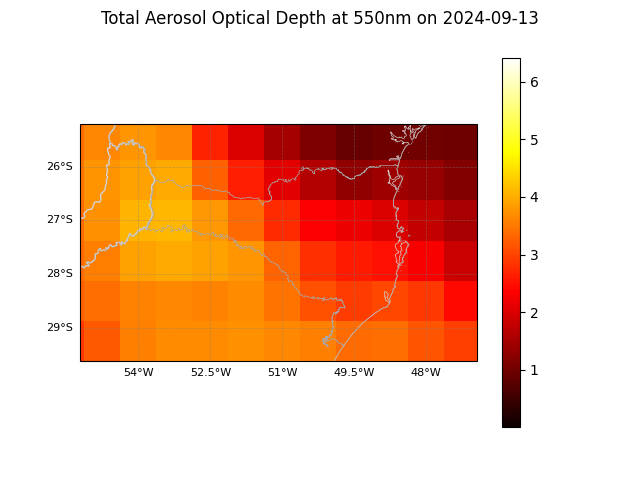
\includegraphics[width=\textwidth, trim=0cm 0cm 0cm 1cm, clip]{images/aod550_2024-09-13_regiao.png}
		\caption{AOD Total - 2024-09-13}
		\label{fig:aod_diario}
	\end{subfigure}
	\hfill
	\begin{subfigure}[b]{0.48\textwidth}
		\centering
		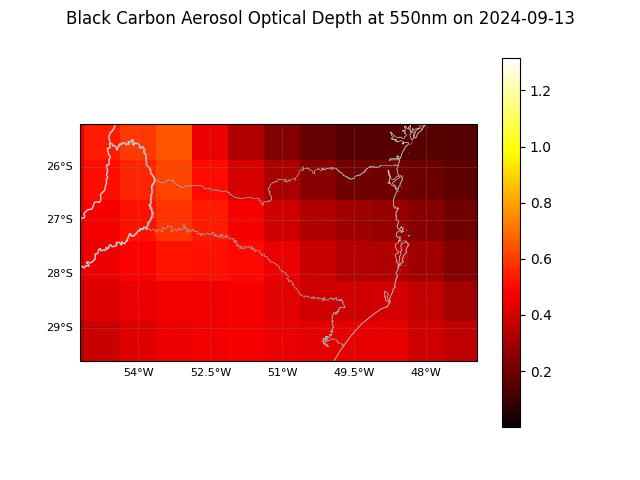
\includegraphics[width=\textwidth, trim=0cm 0cm 0cm 1cm, clip]{images/bcaod550_2024-09-13_regiao.png}
		\caption{Black Carbon AOD - 2024-09-13}
		\label{fig:bcaod_diario}
	\end{subfigure}
	
	\centering
	\begin{subfigure}[b]{0.48\textwidth}
		\centering
		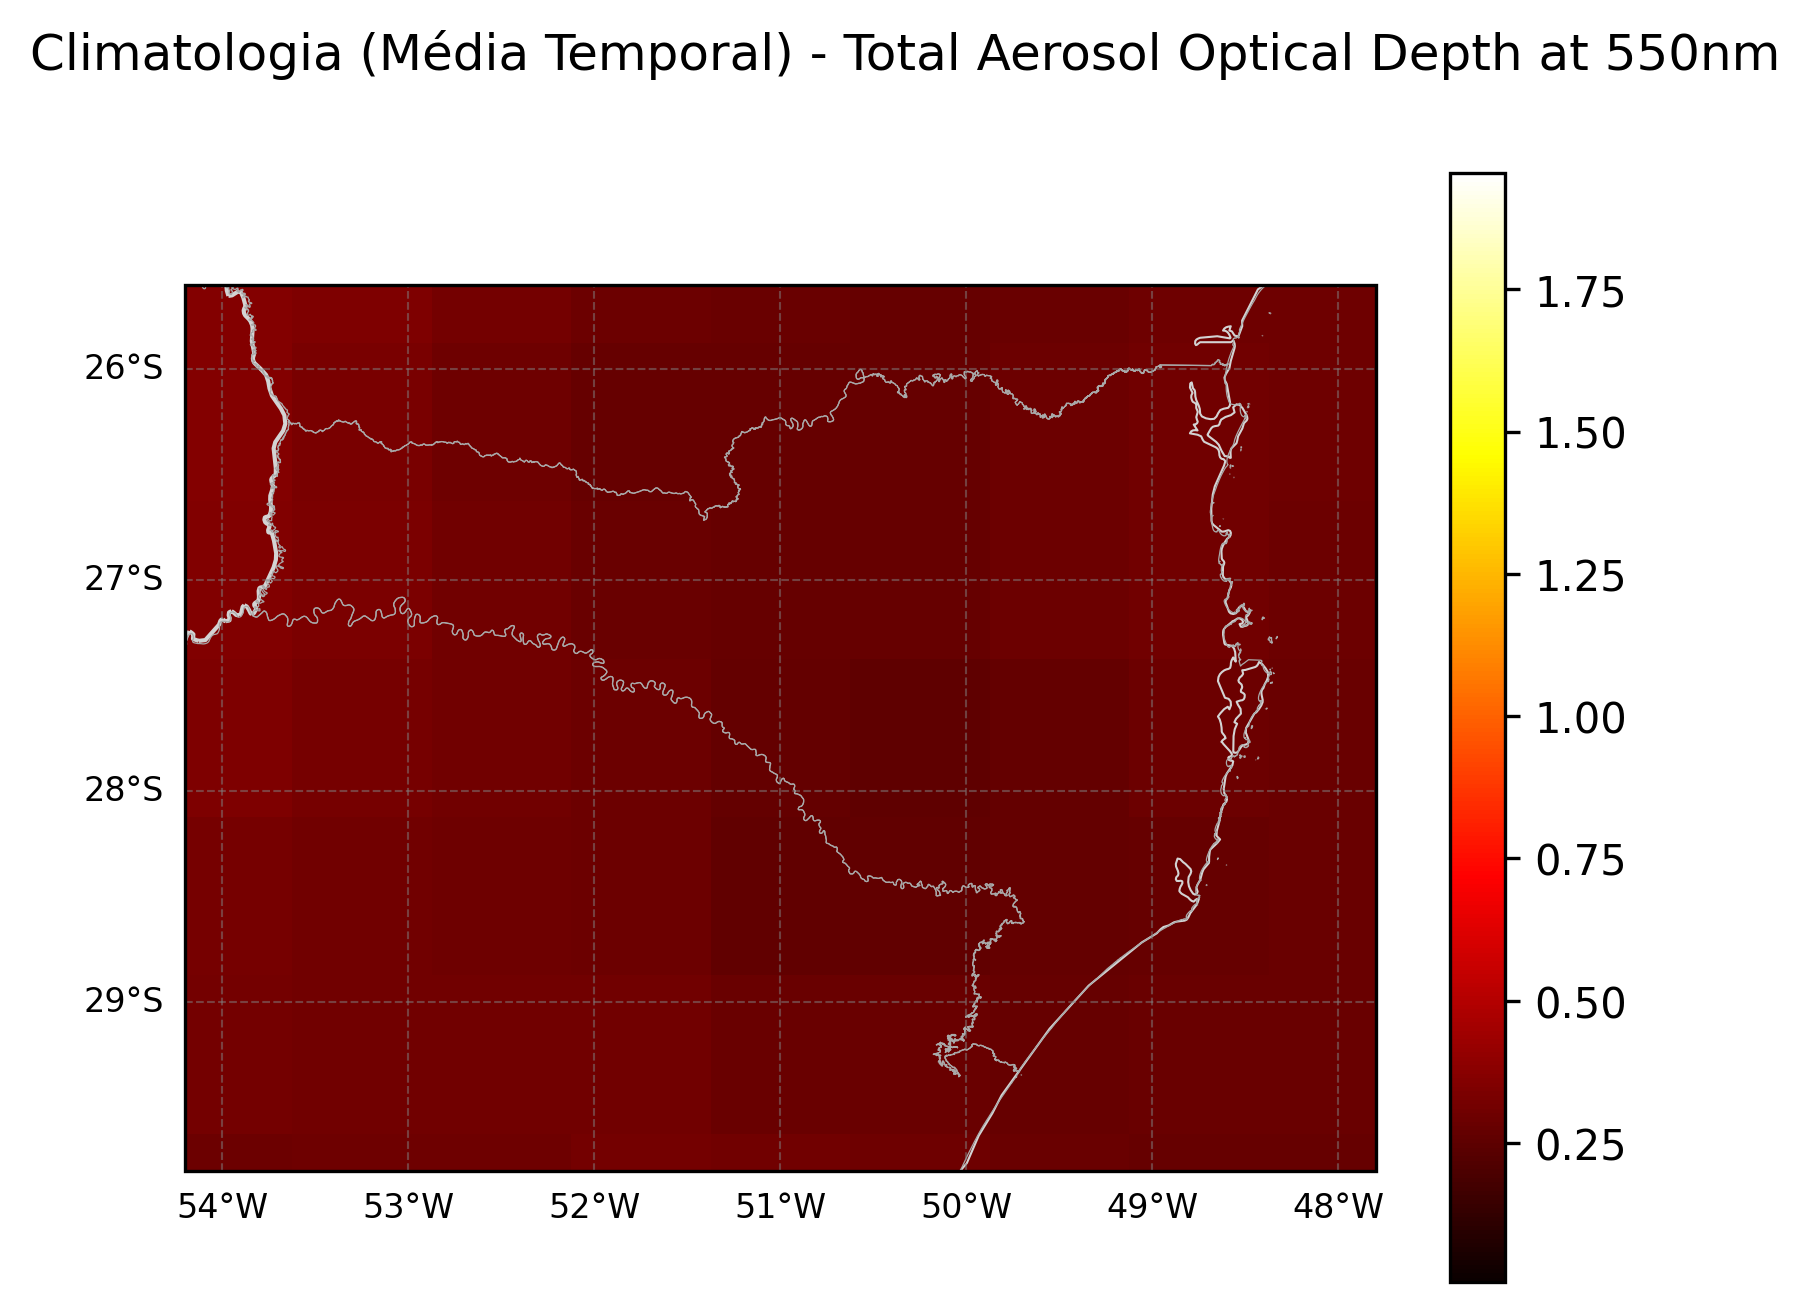
\includegraphics[width=\textwidth, trim=0cm 0cm 0cm 1cm, clip]{images/aod550_climatologia_regiao.png}
		\caption{AOD Total - Média para setembro}
		\label{fig:aod_clima}
	\end{subfigure}
	\hfill
	\begin{subfigure}[b]{0.48\textwidth}
		\centering
		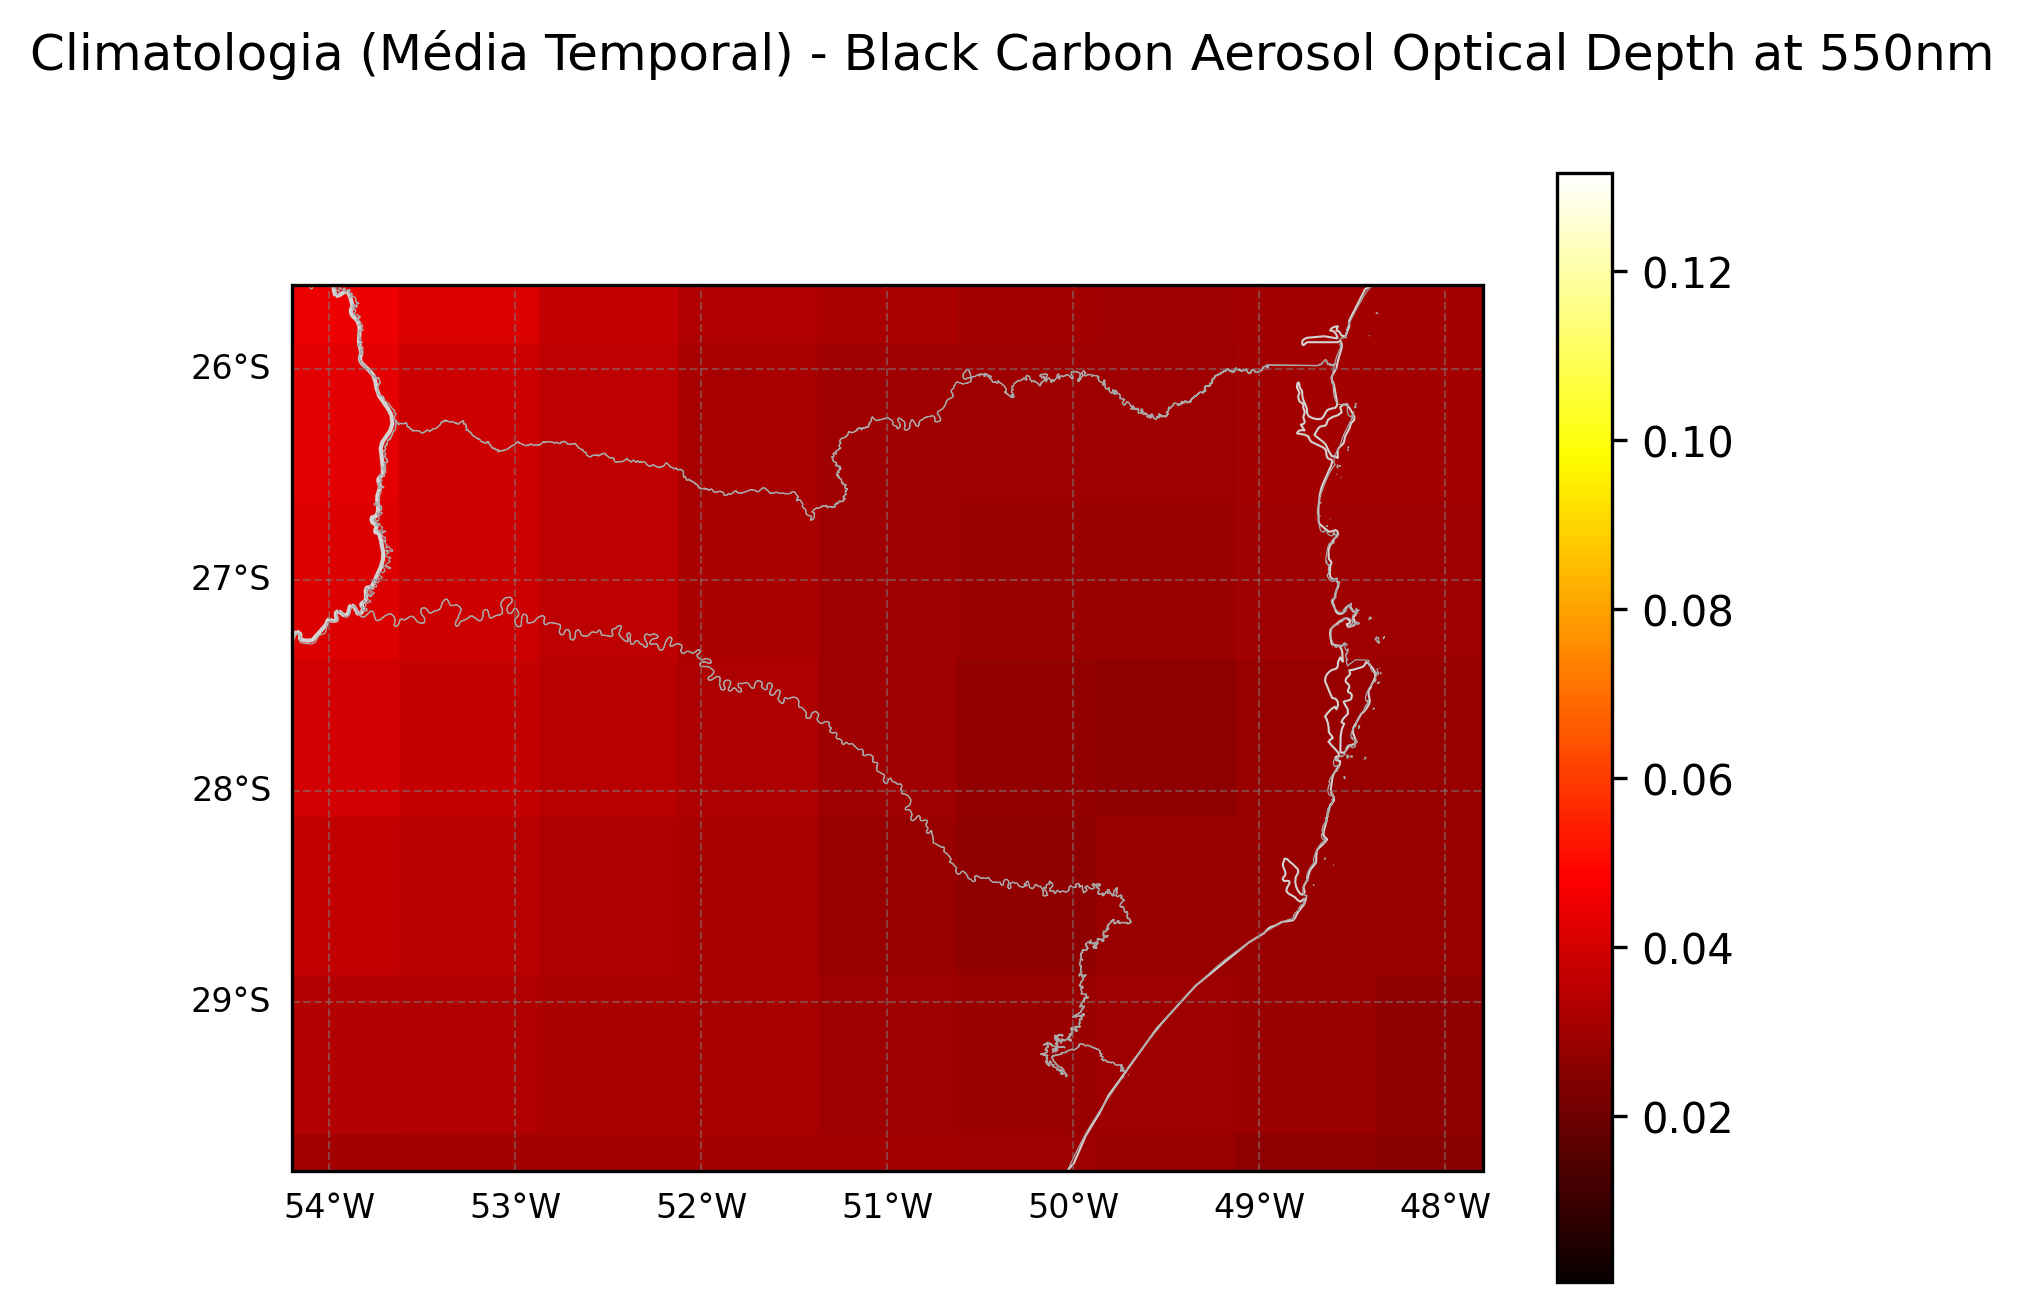
\includegraphics[width=\textwidth, trim=0cm 0cm 0cm 1cm, clip]{images/bcaod550_climatologia_regiao.png}
		\caption{Black Carbon AOD - Média para setembro}
		\label{fig:bcaod_clima}
	\end{subfigure}
	
	\caption{Profundidades Ópticas em 550nm (a) total e (b) específica de Black Carbon sobre o estado de Santa Catarina em 13 de setembro de 2024. Média mensal para setembro de profundidades ópticas em 550nm (c) total e (d) específica de Black Carbon sobre o estado de Santa Catarina entre os anos de 2003 e 2023. Elaboração do autor com dados da reanálise CAMS EAC4.}
	\label{fig:aod_diario_conjunto}
\end{figure}

Assumindo o dia 13 como ponto de referência, foi analisado o perfil da atmosfera nos dias que antecederam essa data. Entre as Figuras \ref{fig:sinotica_20240905_1200} e \ref{fig:sinotica_20240913_1200} estão dispostos mapas de variáveis meteorológicas para a América do Sul entre os dias 05 e 13 de setembro de 2024. É possível identificar um sistema de alta pressão em superfície posicionado próximo à latitude de 40°S, tanto pelos valores de pressão a nível médio do mar e escoamento a 10m, quanto pelos gradientes de temperatura do ponto de orvalho. Entre os 8 dias analisados, o deslocamento desse sistema para oeste se deu entre 140° e 120° O. Ao longo do nível de 500 hPa, identifica-se um cavado à frente do sistema de alta anteriormente identificado, o que corrobora com um bloqueio de tipo ômega citado na seção \ref{sec:bloqueio}. 

Na Figura \ref{fig:goesgeral}, estão dispostas as imagens geradas pelo canal 13 do satélite GOES16, onde as cores mais quentes significam topos de nuvens mais altos, ou seja, maior atividade convectiva ocorrendo naquele local. Ao longo do período analisado, não foram identificados padrões de nuvens que se assemelhem à passagem de sistemas frontais pela região sul do Brasil após o dia 05 de setembro.



\begin{figure}[htb]
	\centering	
	\begin{subfigure}[b]{\textwidth}
		\centering
		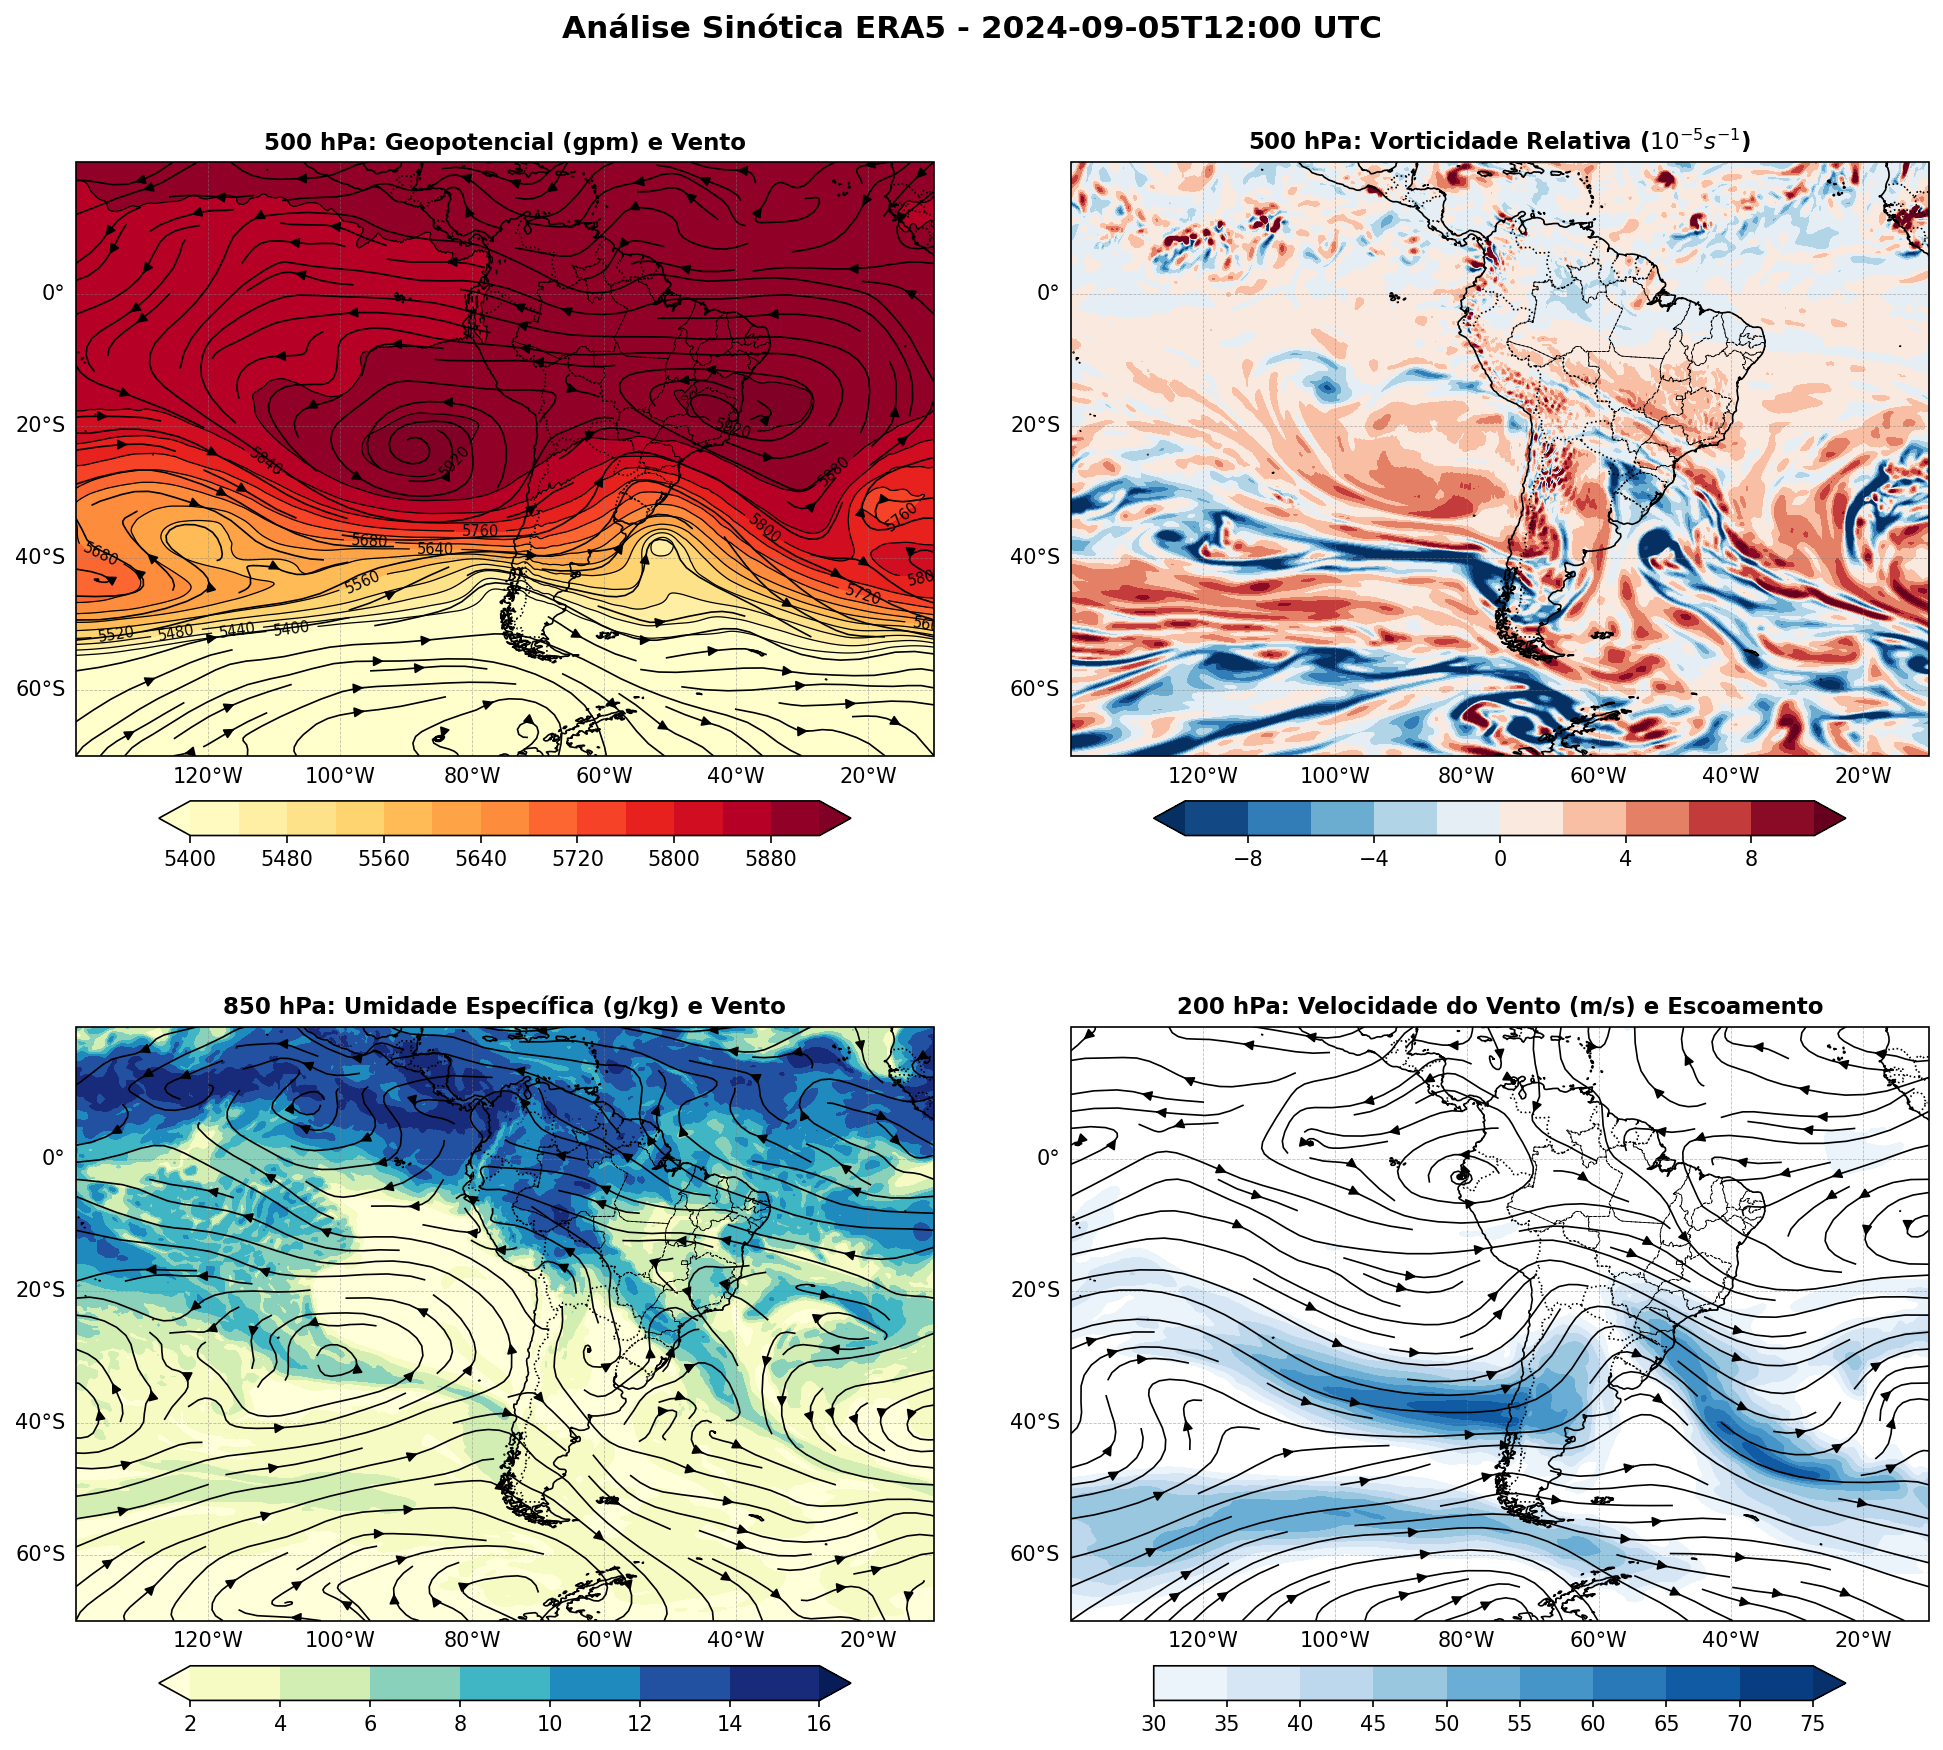
\includegraphics[width = 0.48\textwidth, trim=0cm 0cm 0cm 2cm, clip]{images/sinotica_20240905_1200.png}
		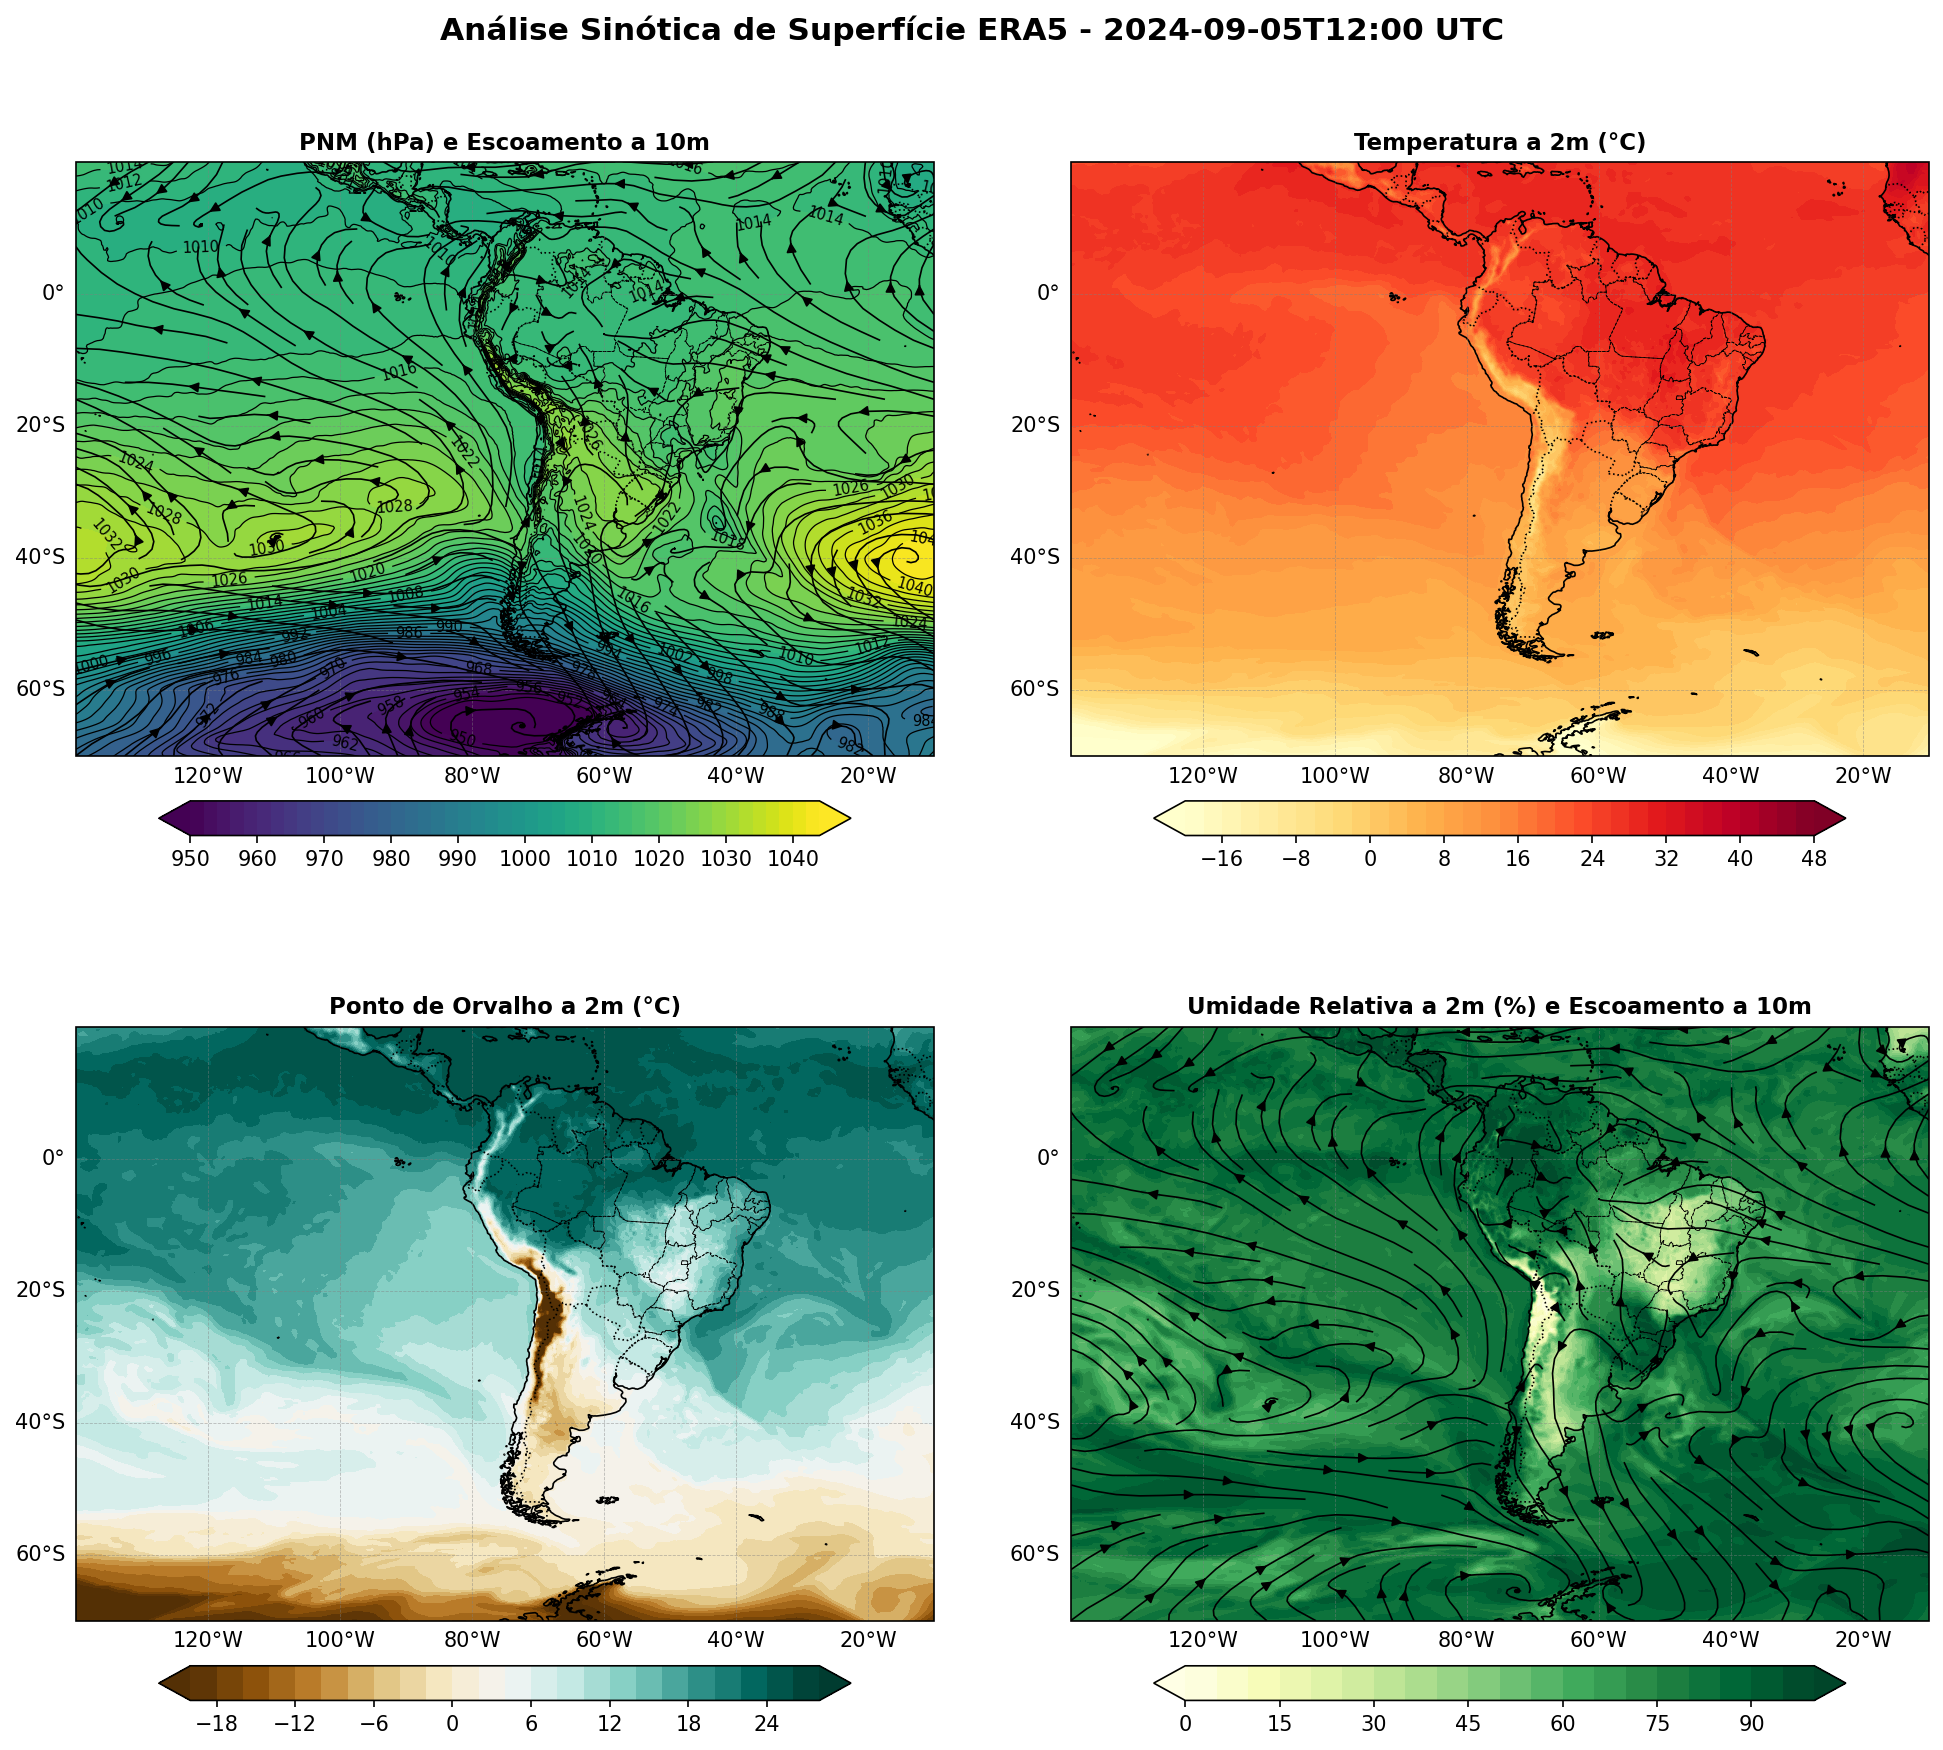
\includegraphics[width = 0.48\textwidth, trim=0cm 0cm 0cm 2cm, clip]{images/superficie_20240905_1200.png}
	\end{subfigure}
		\caption{Análise Sinótica ERA5 - 2024-09-05T12:00 UTC}
		\label{fig:sinotica_20240905_1200}
\end{figure}


\begin{figure}[htb]
	\centering	
	\begin{subfigure}[b]{\textwidth}
		\centering
		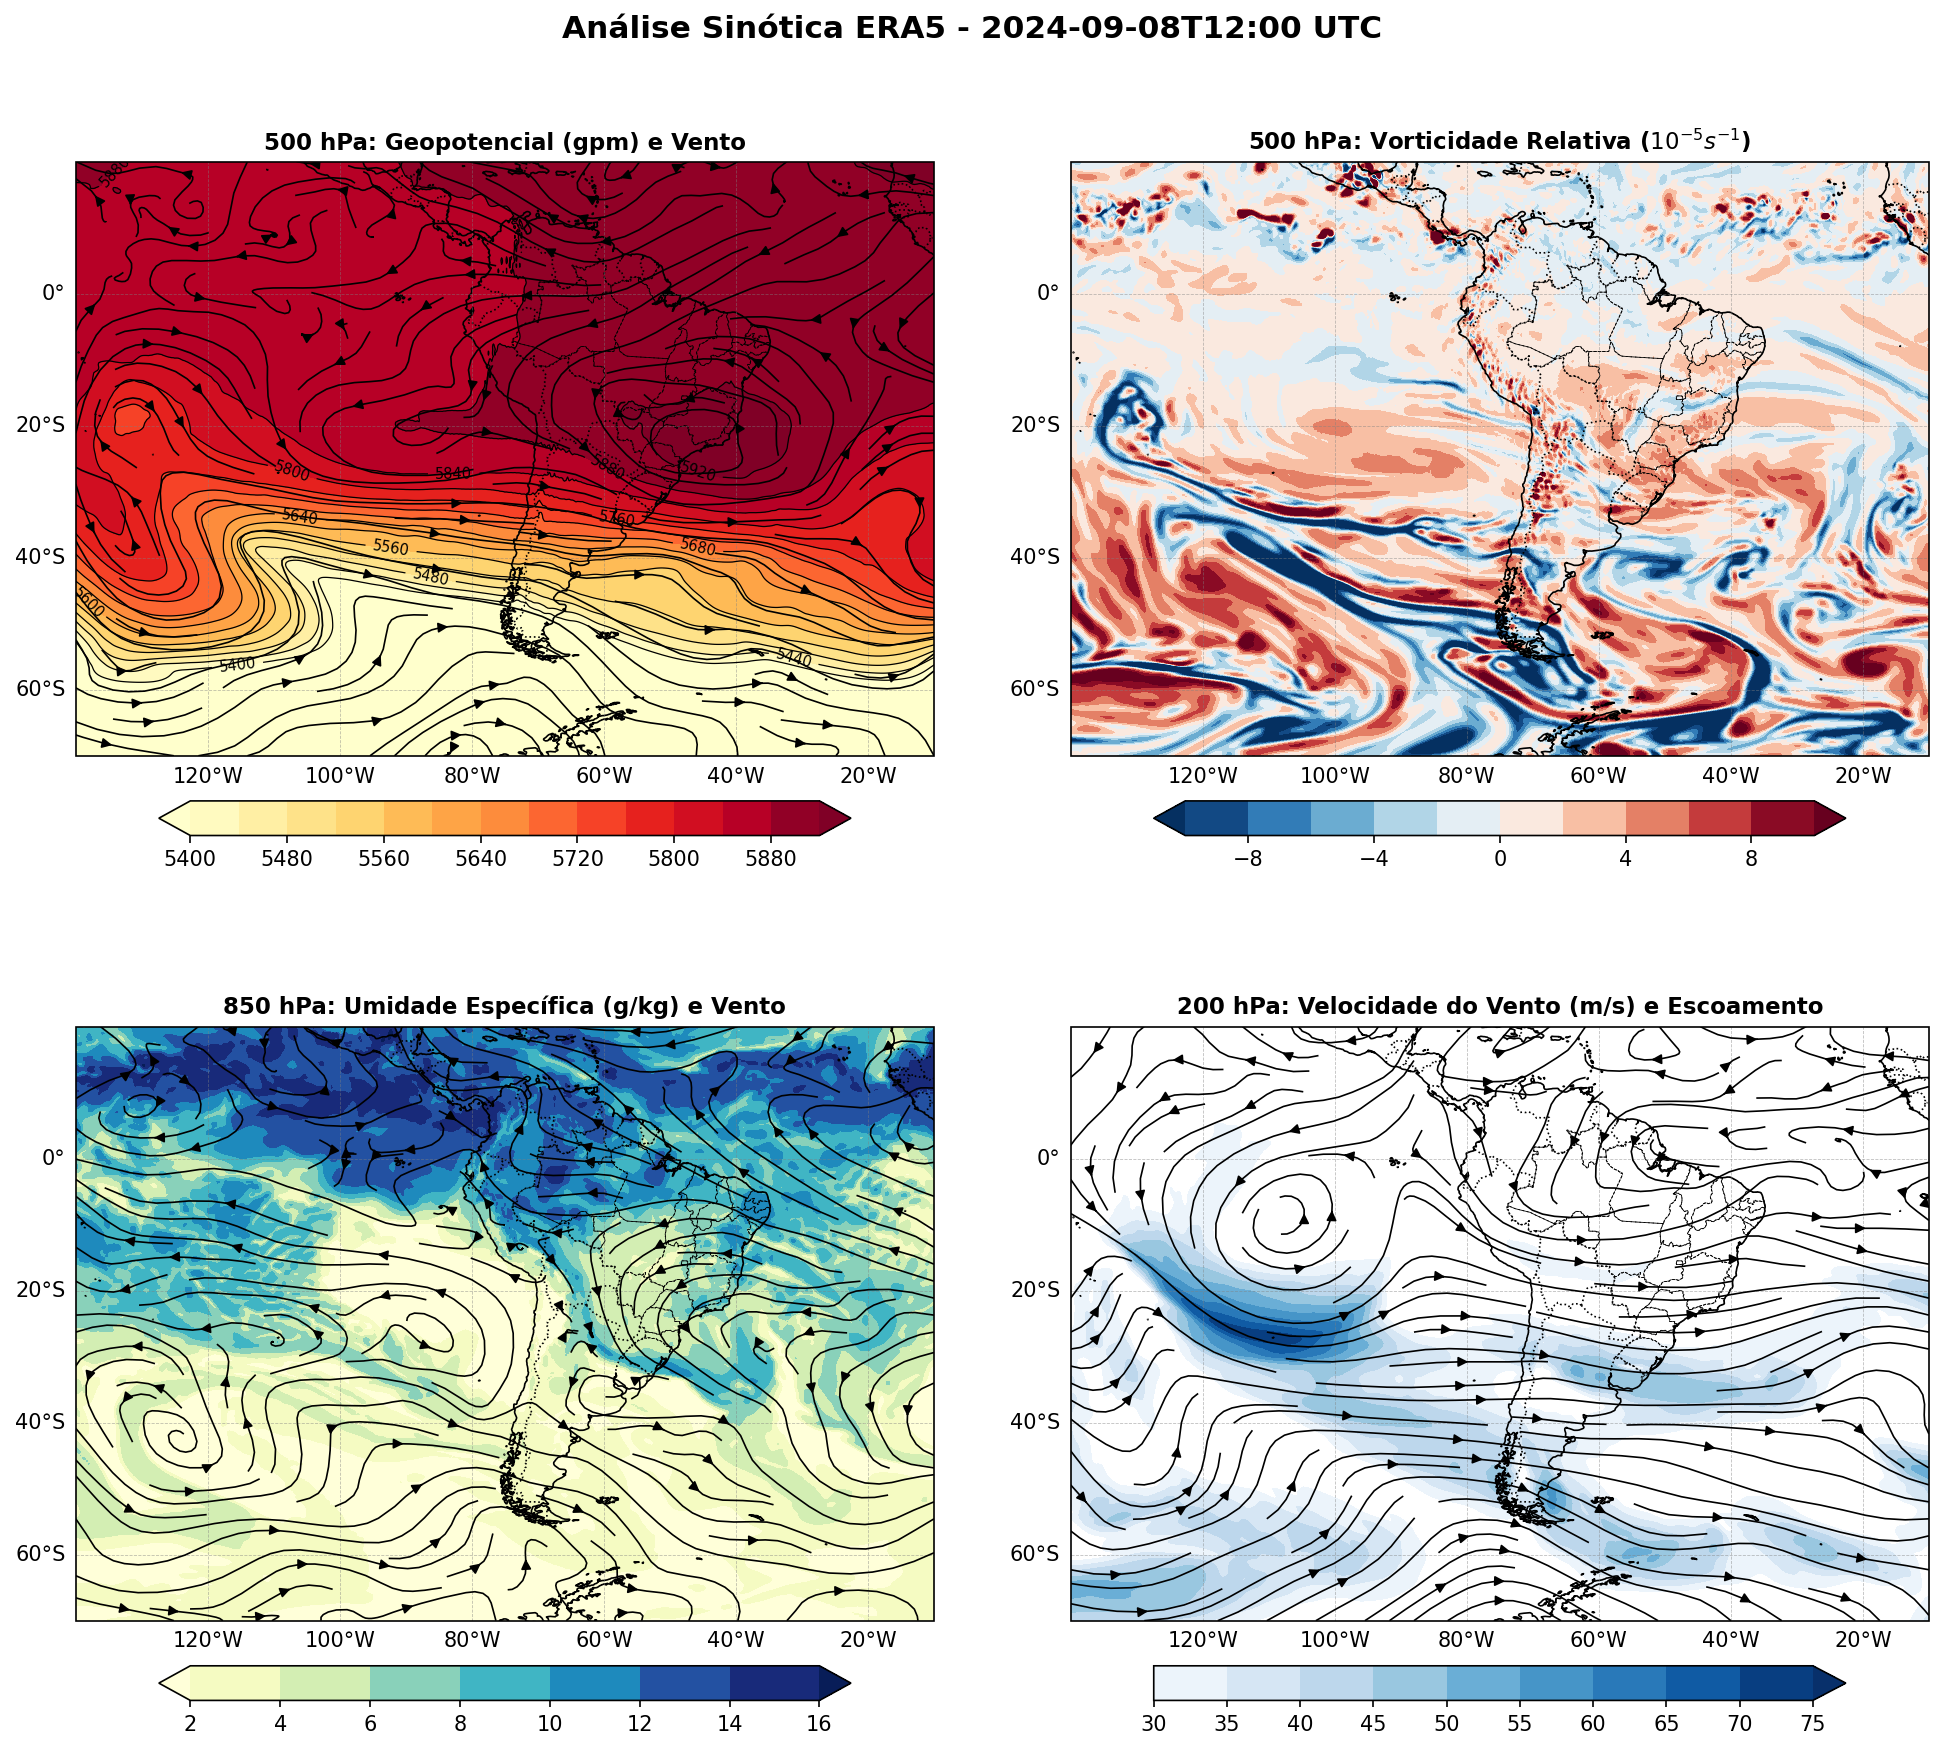
\includegraphics[width = 0.48\textwidth, trim=0cm 0cm 0cm 2cm, clip]{images/sinotica_20240908_1200.png}
		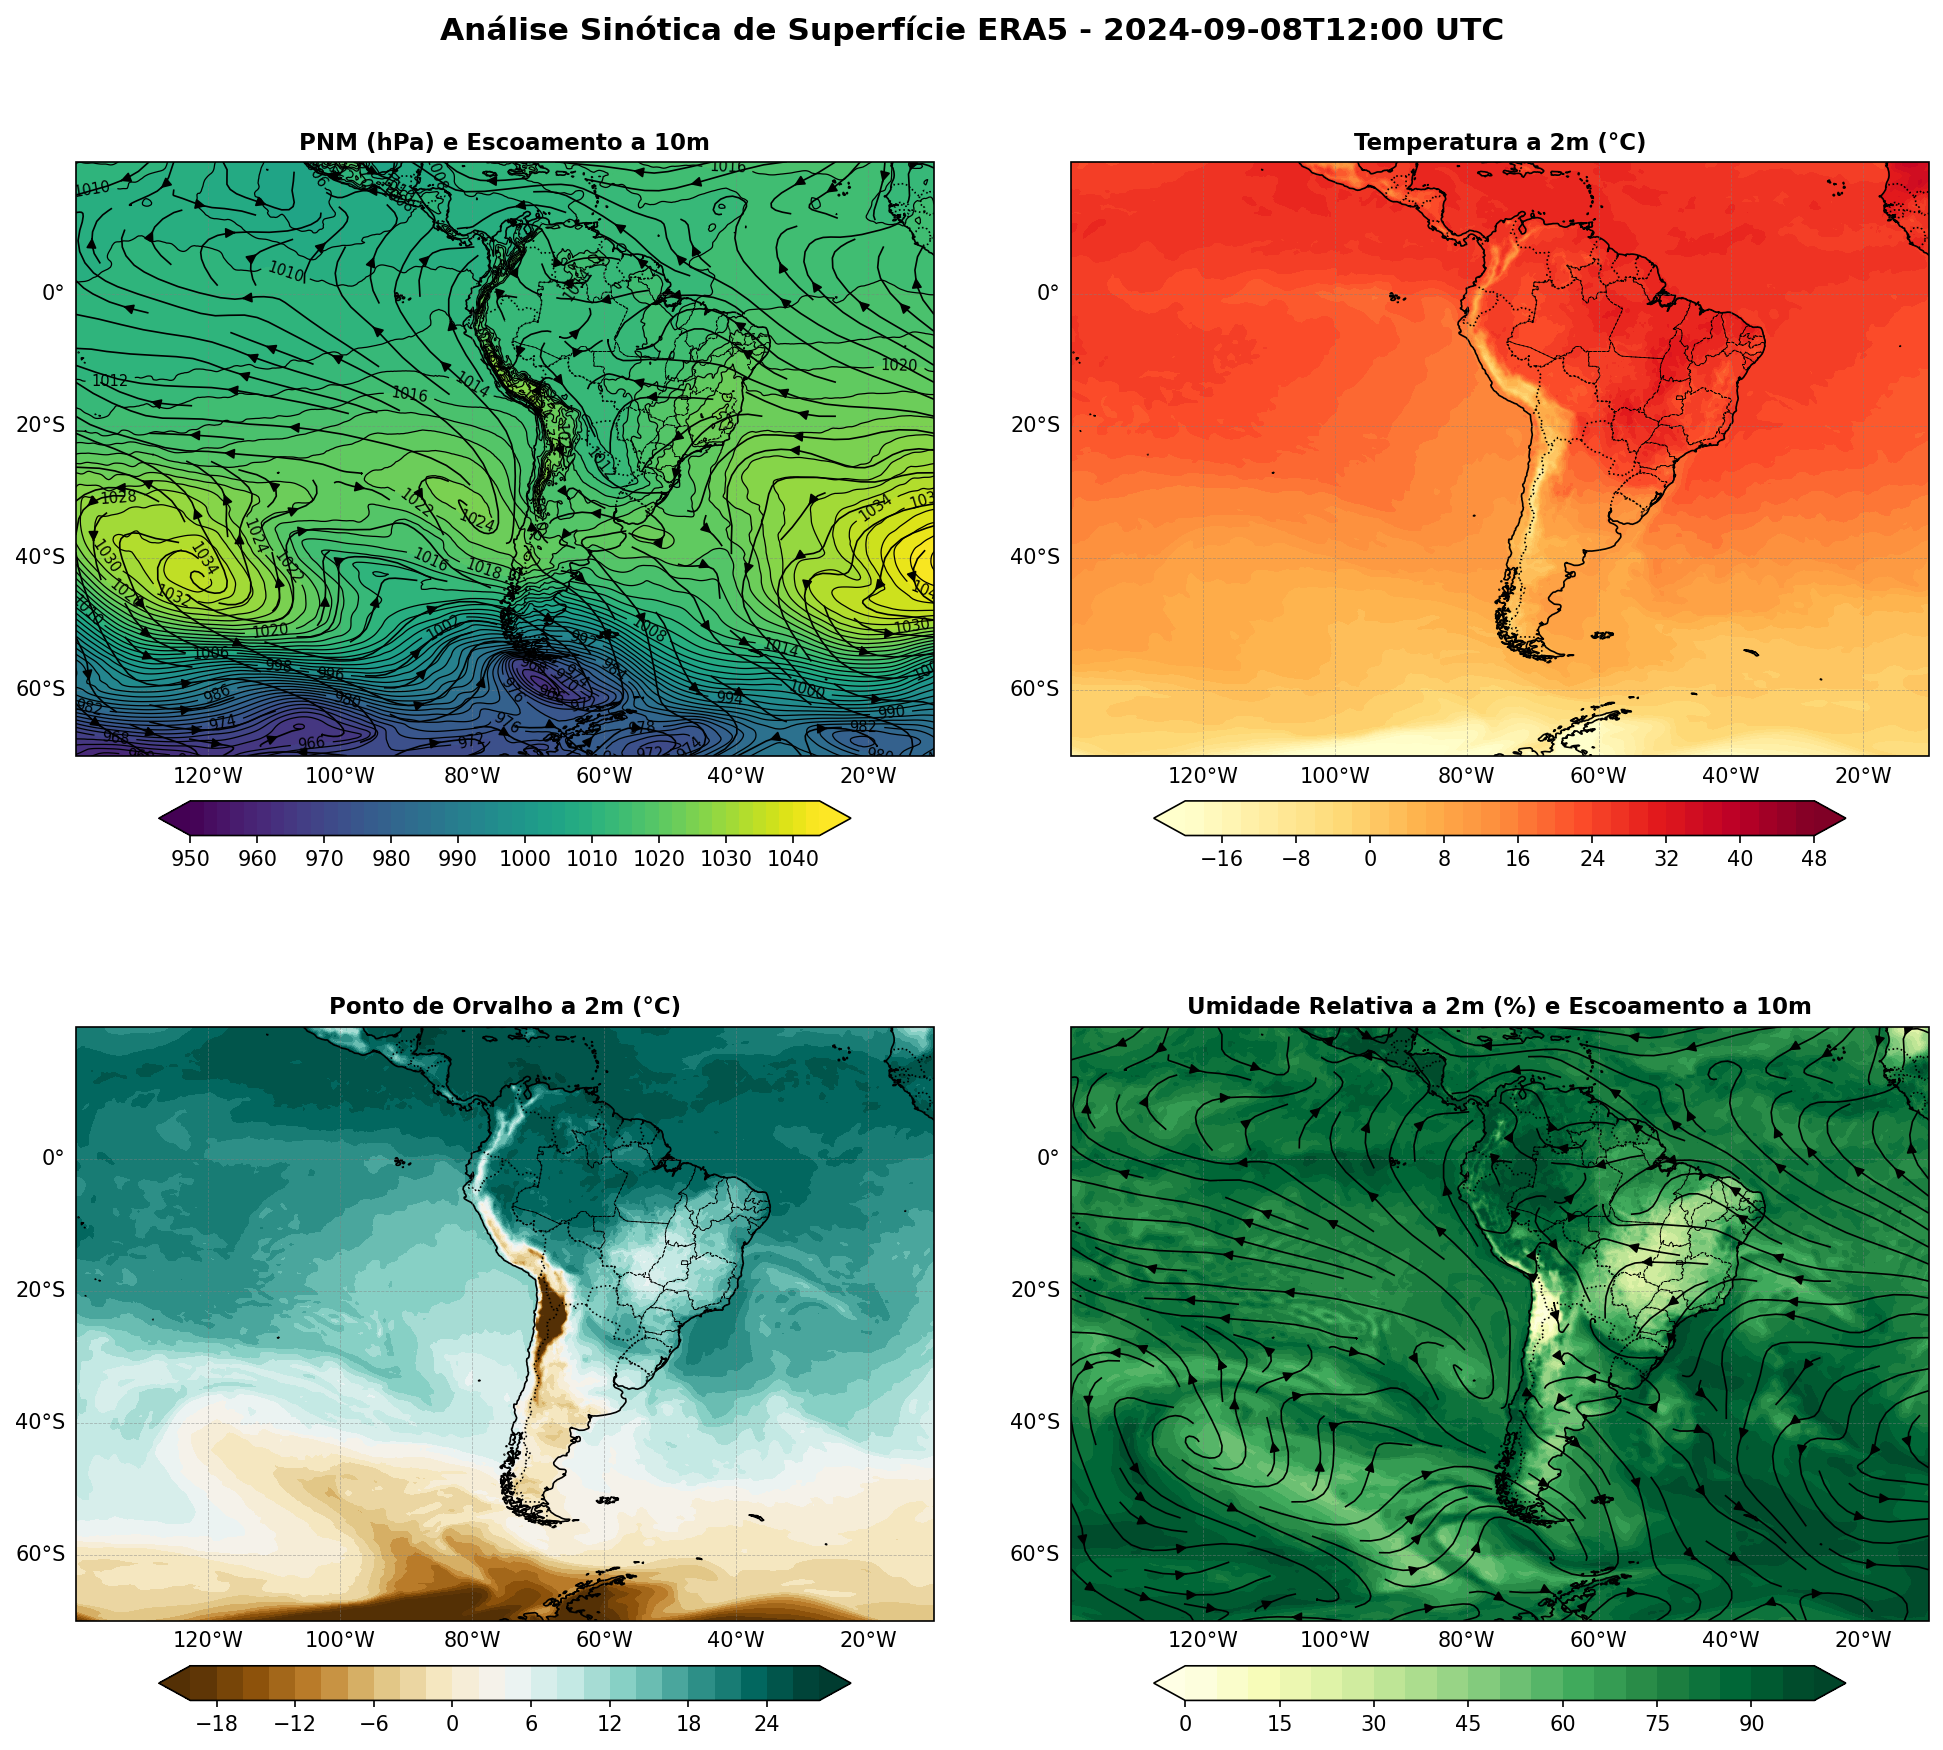
\includegraphics[width = 0.48\textwidth, trim=0cm 0cm 0cm 2cm, clip]{images/superficie_20240908_1200.png}
	\end{subfigure}
	\caption{Análise Sinótica ERA5 - 2024-09-08T12:00 UTC}
	\label{fig:sinotica_20240908_1200}
\end{figure}

\begin{figure}[htb]
	\centering	
	\begin{subfigure}[b]{\textwidth}
		\centering
		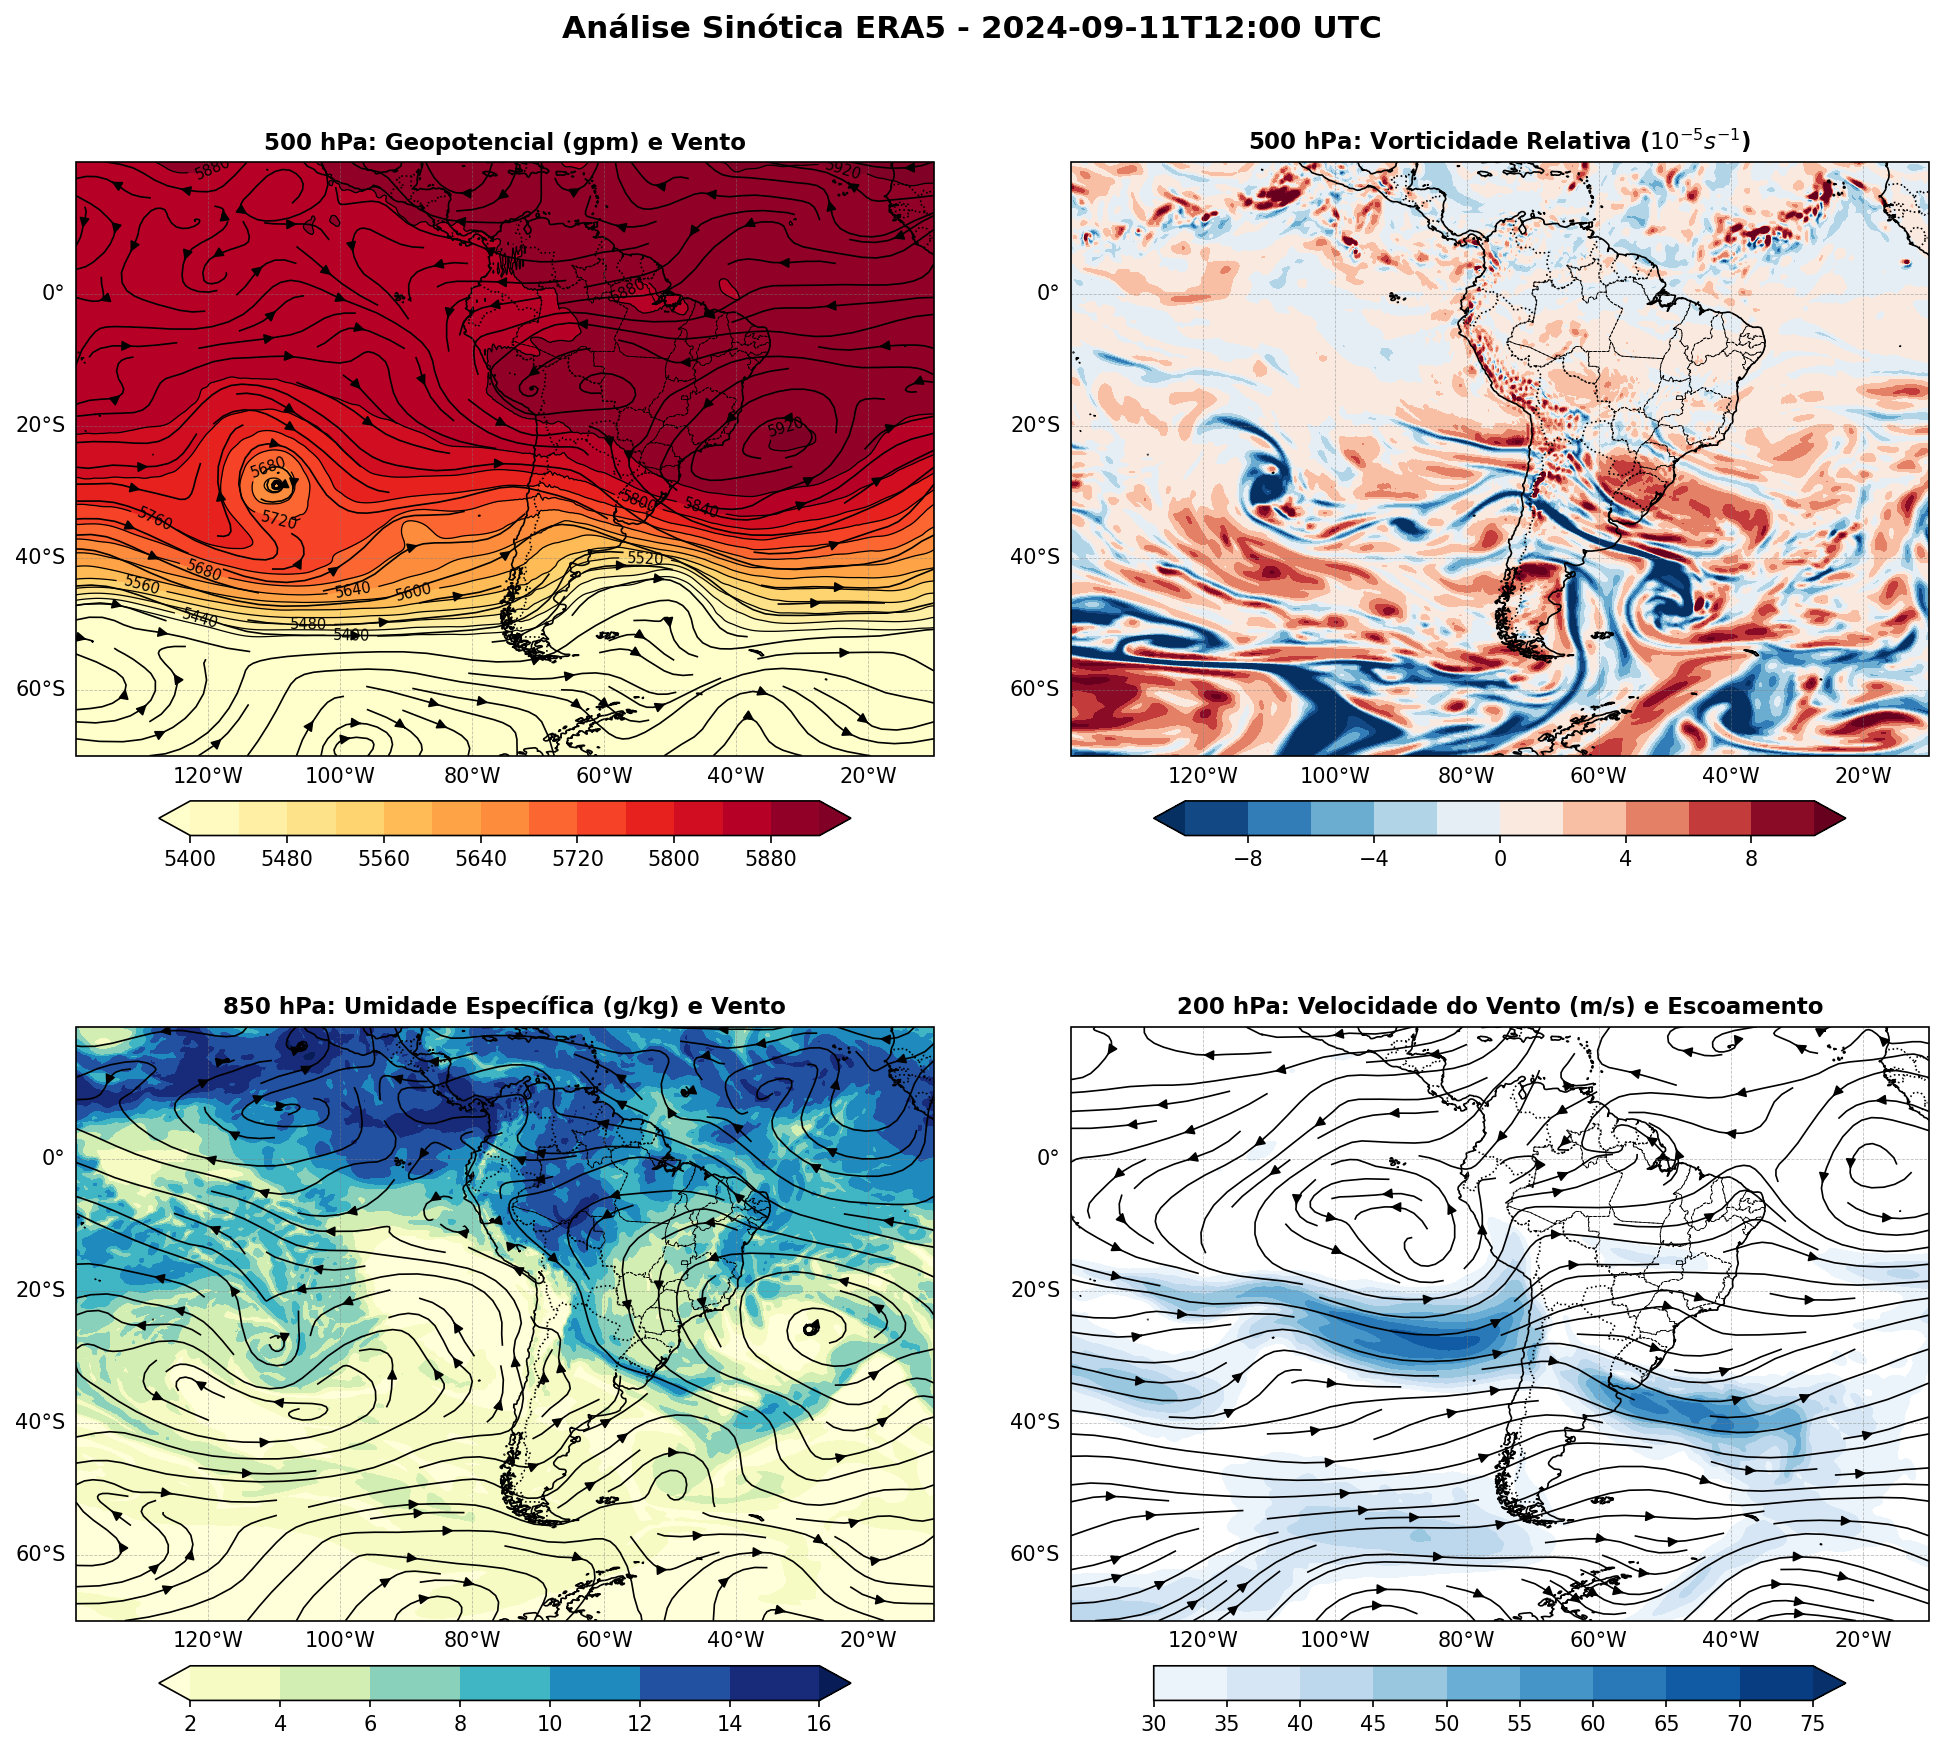
\includegraphics[width = 0.48\textwidth, trim=0cm 0cm 0cm 2cm, clip]{images/sinotica_20240911_1200.png}
		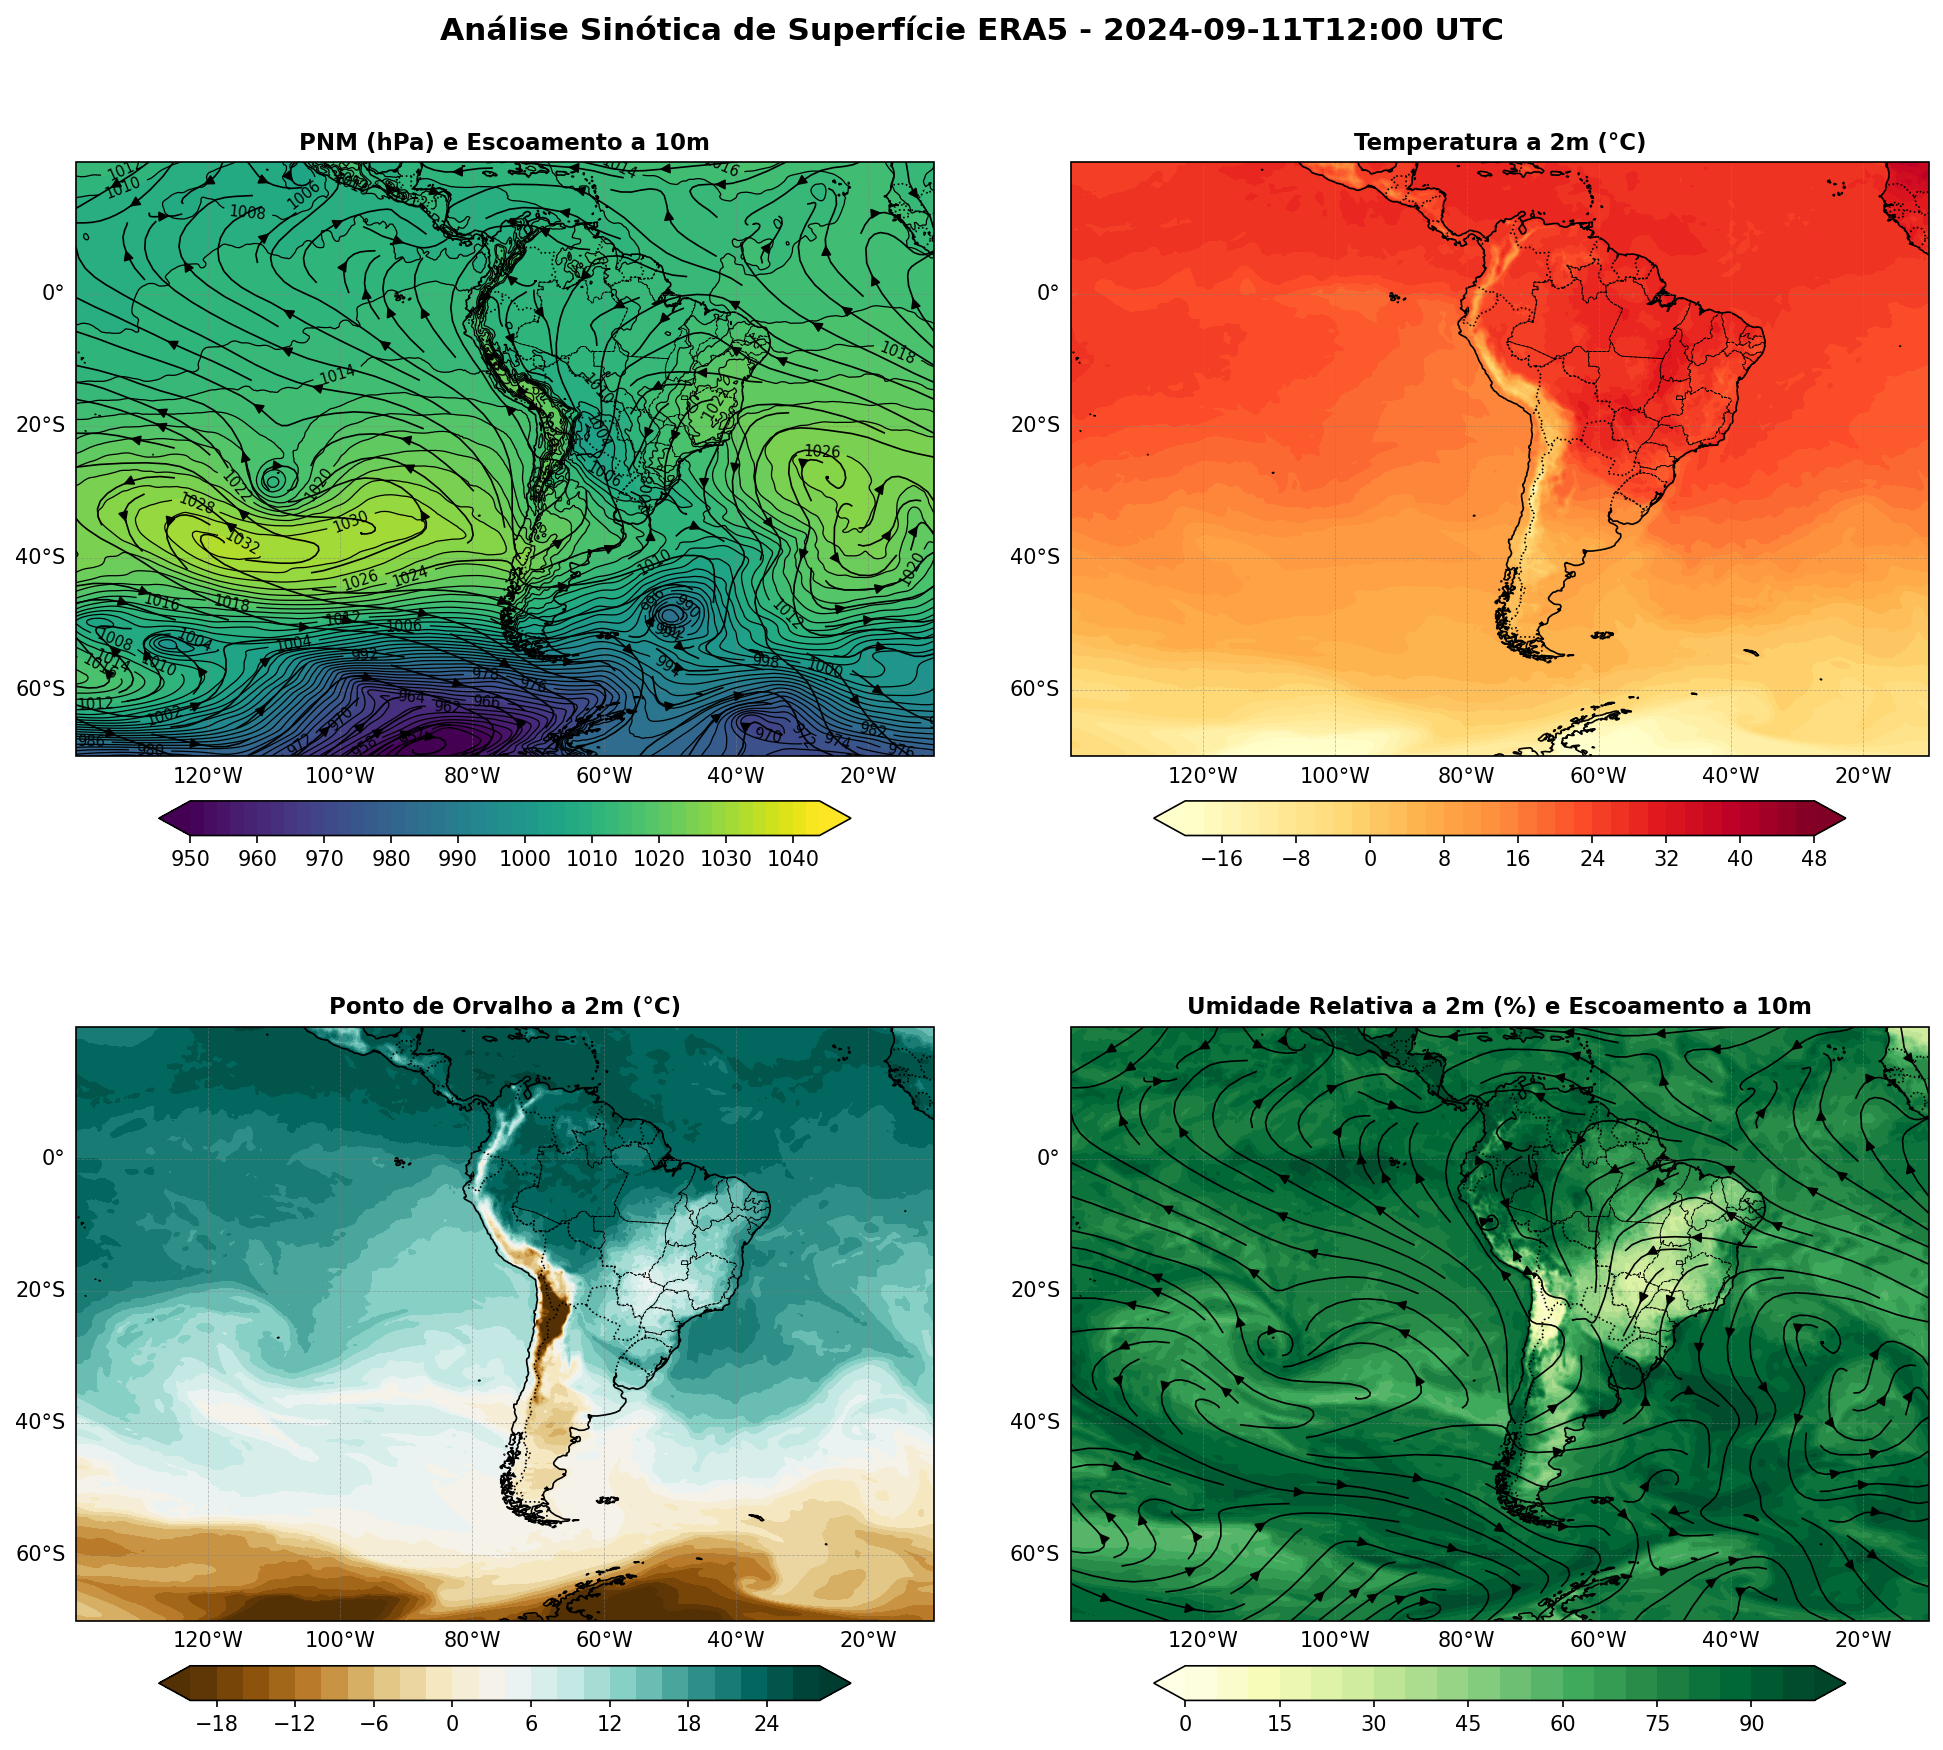
\includegraphics[width = 0.48\textwidth, trim=0cm 0cm 0cm 2cm, clip]{images/superficie_20240911_1200.png}
	\end{subfigure}
	\caption{Análise Sinótica ERA5 - 2024-09-11T11:00 UTC}
	\label{fig:sinotica_20240908_1100}
\end{figure}



\begin{figure}[htb]
	\centering	
	\begin{subfigure}[b]{\textwidth}
		\centering
		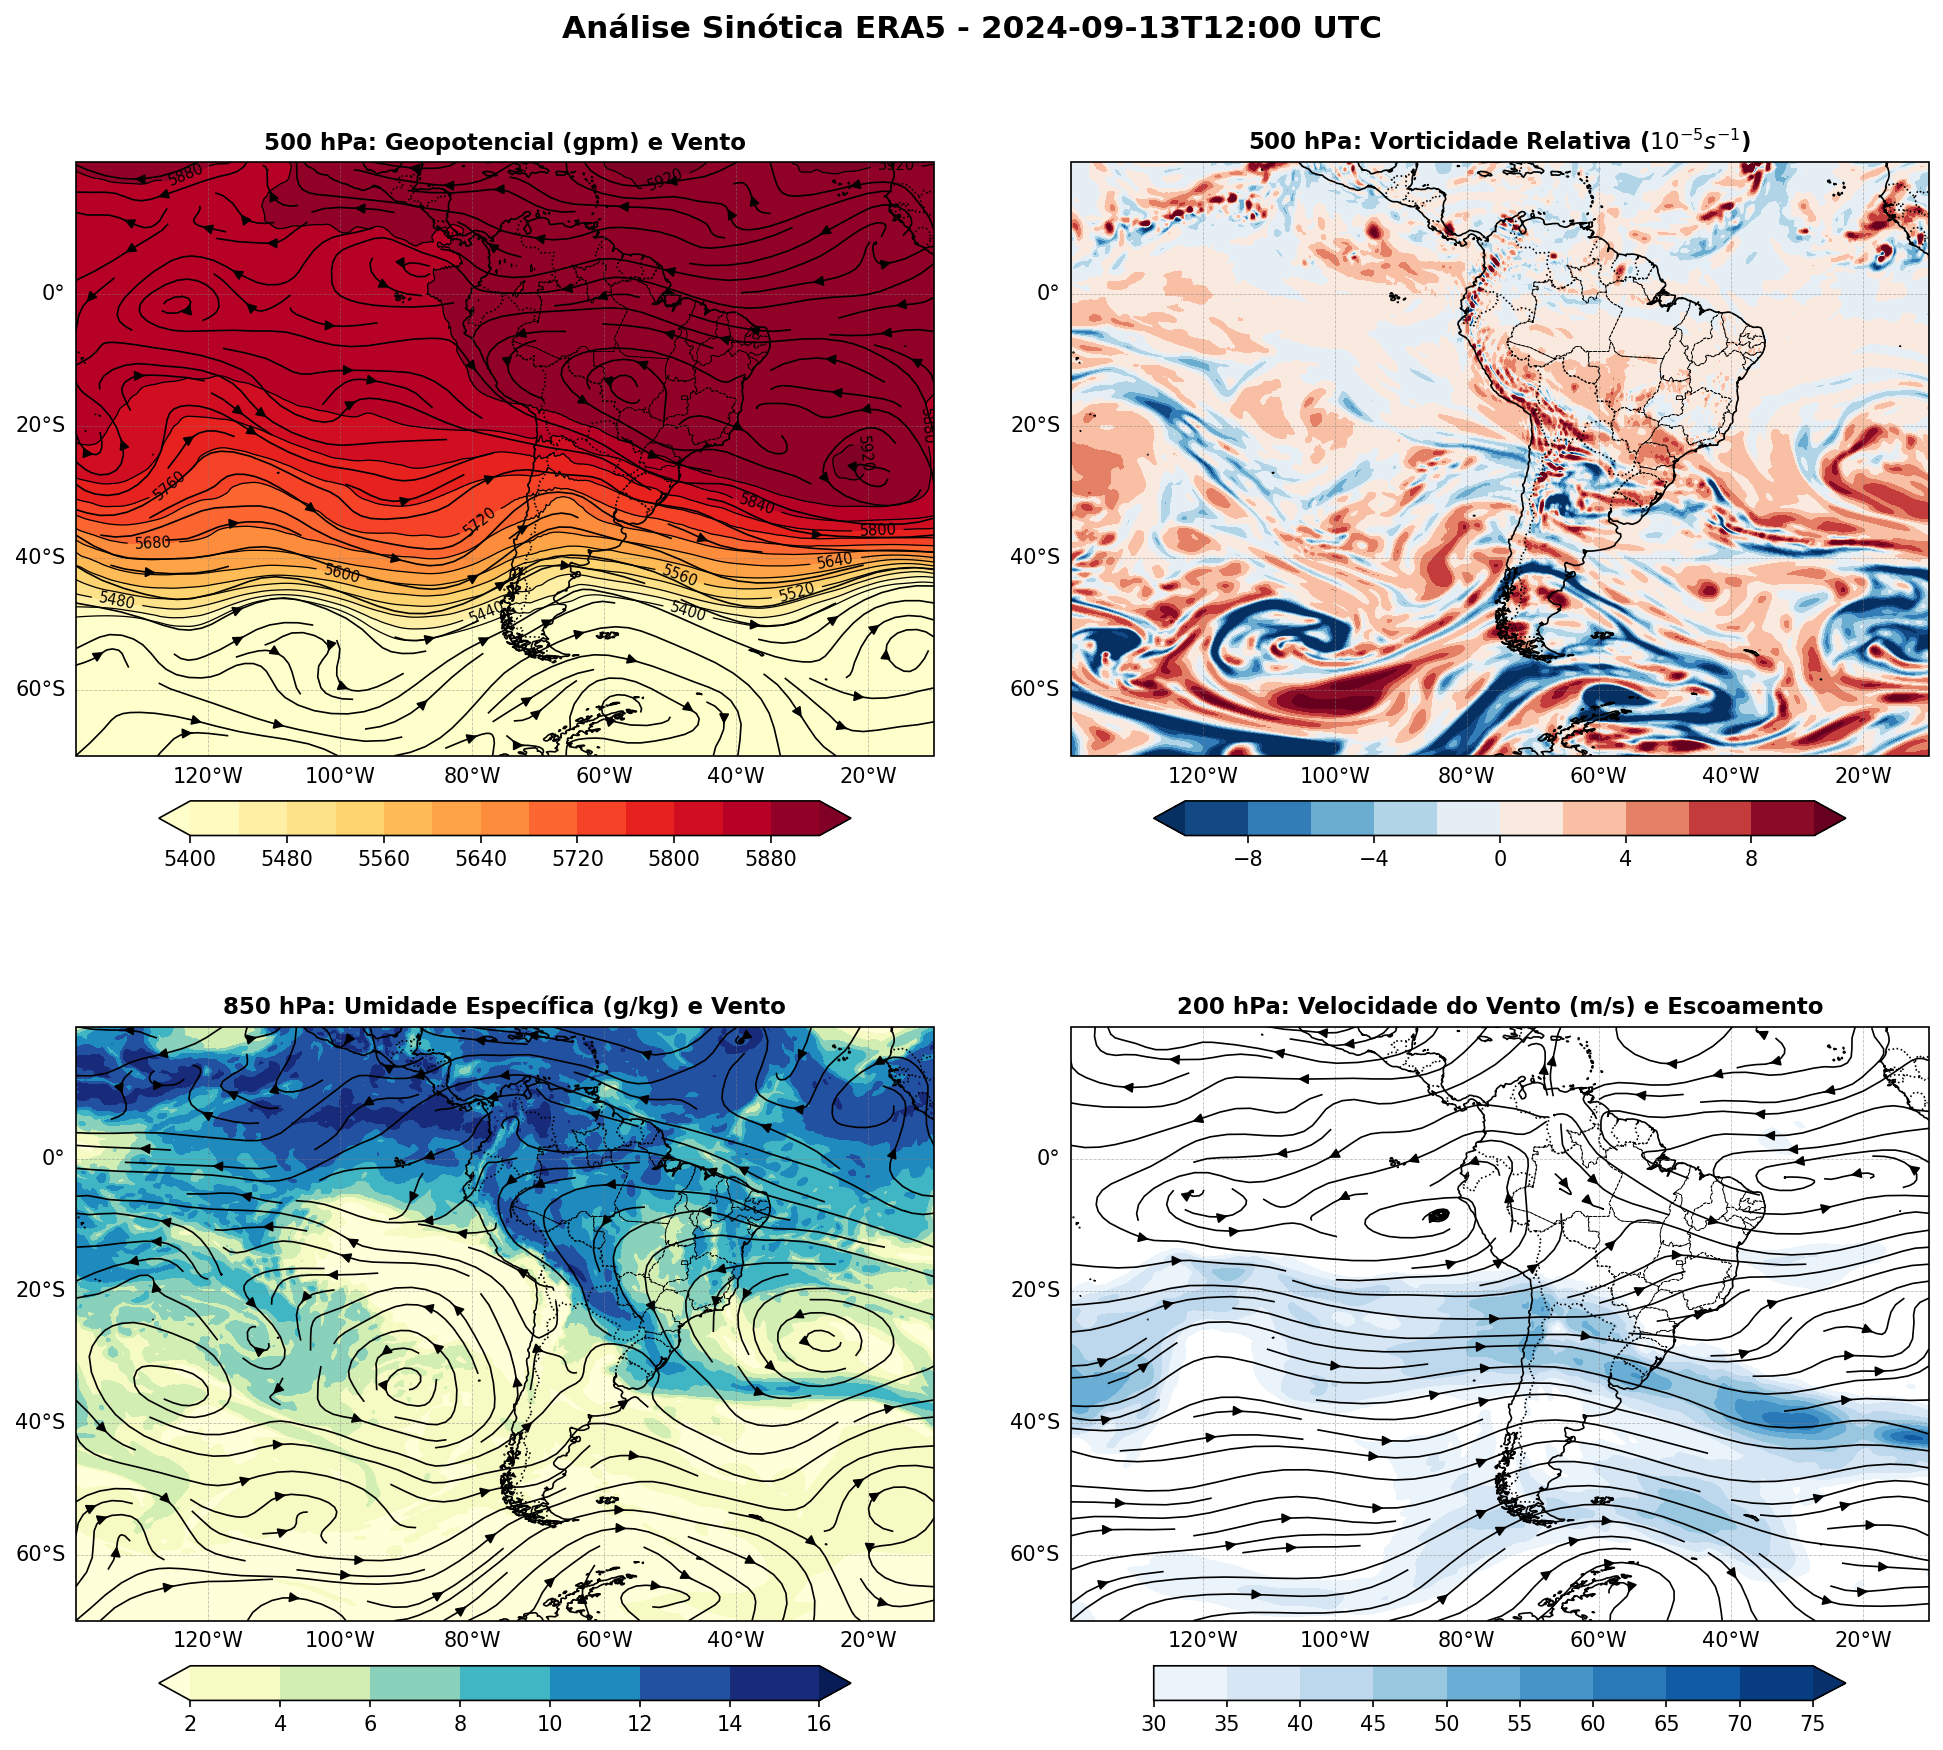
\includegraphics[width = 0.48\textwidth, trim=0cm 0cm 0cm 2cm, clip]{images/sinotica_20240913_1200.png}
		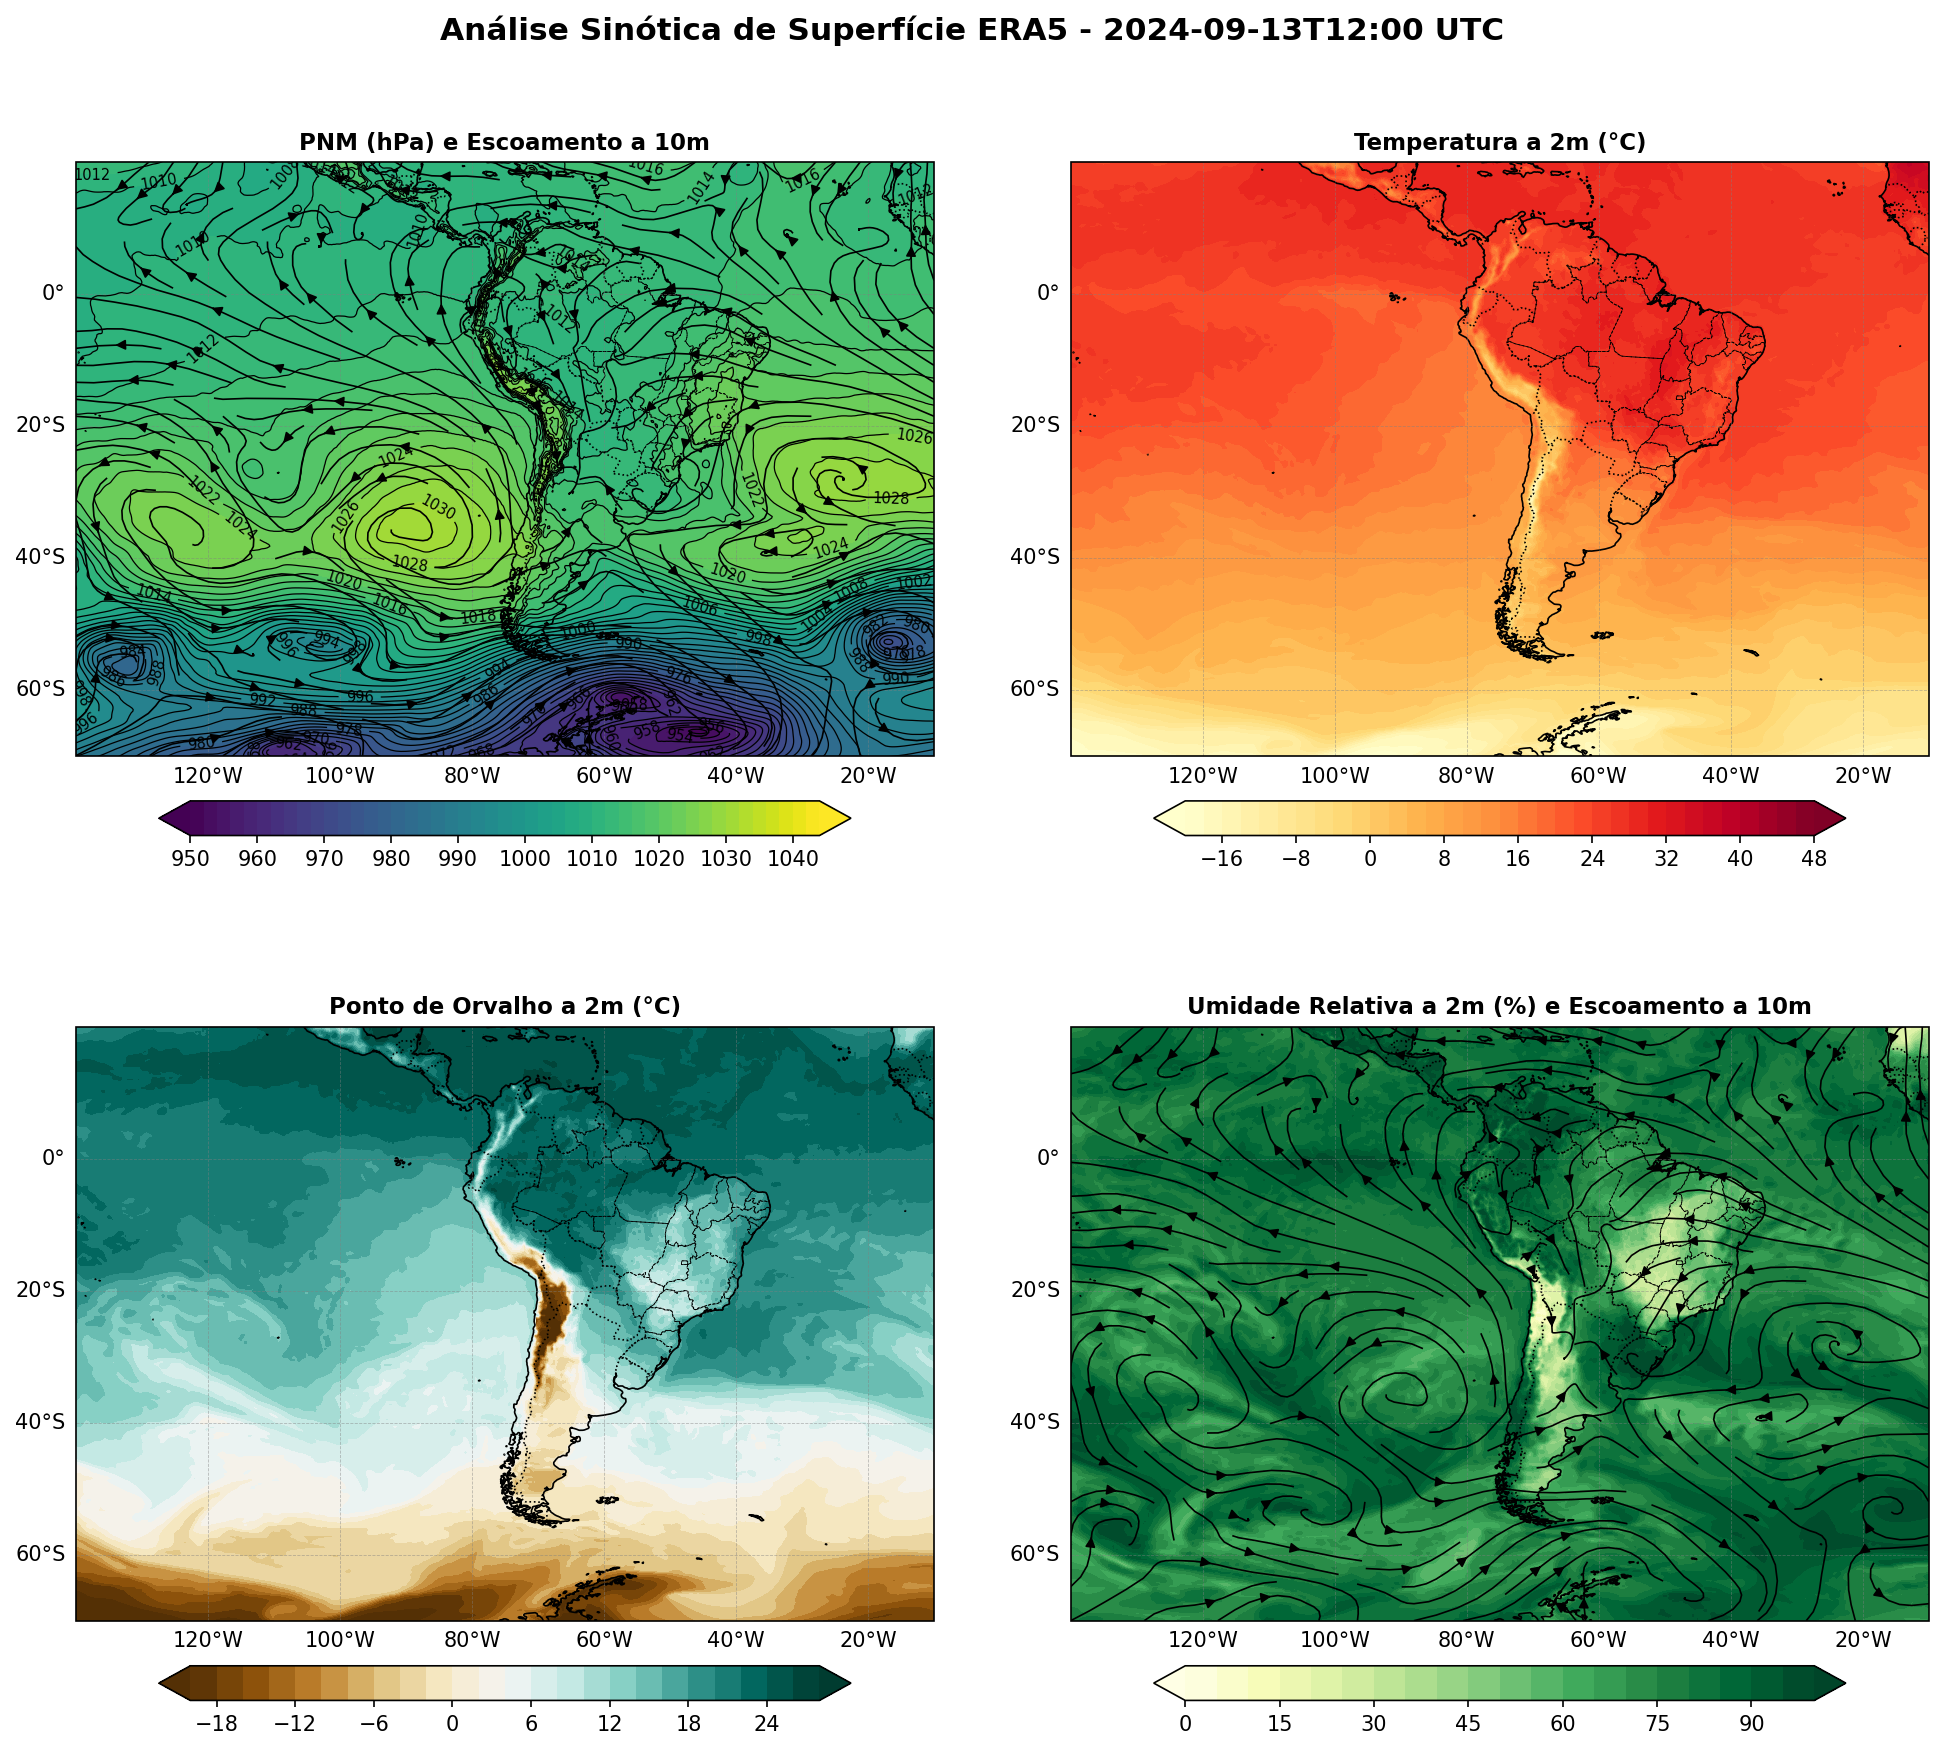
\includegraphics[width = 0.48\textwidth, trim=0cm 0cm 0cm 2cm, clip]{images/superficie_20240913_1200.png}
	\end{subfigure}
	\caption{Análise Sinótica ERA5 - 2024-09-13T12:00 UTC}
	\label{fig:sinotica_20240913_1200}
\end{figure}


\begin{figure}
		\centering
	% --- LINHA 1 ---
	\begin{subfigure}[b]{0.4\textwidth}
	\centering
	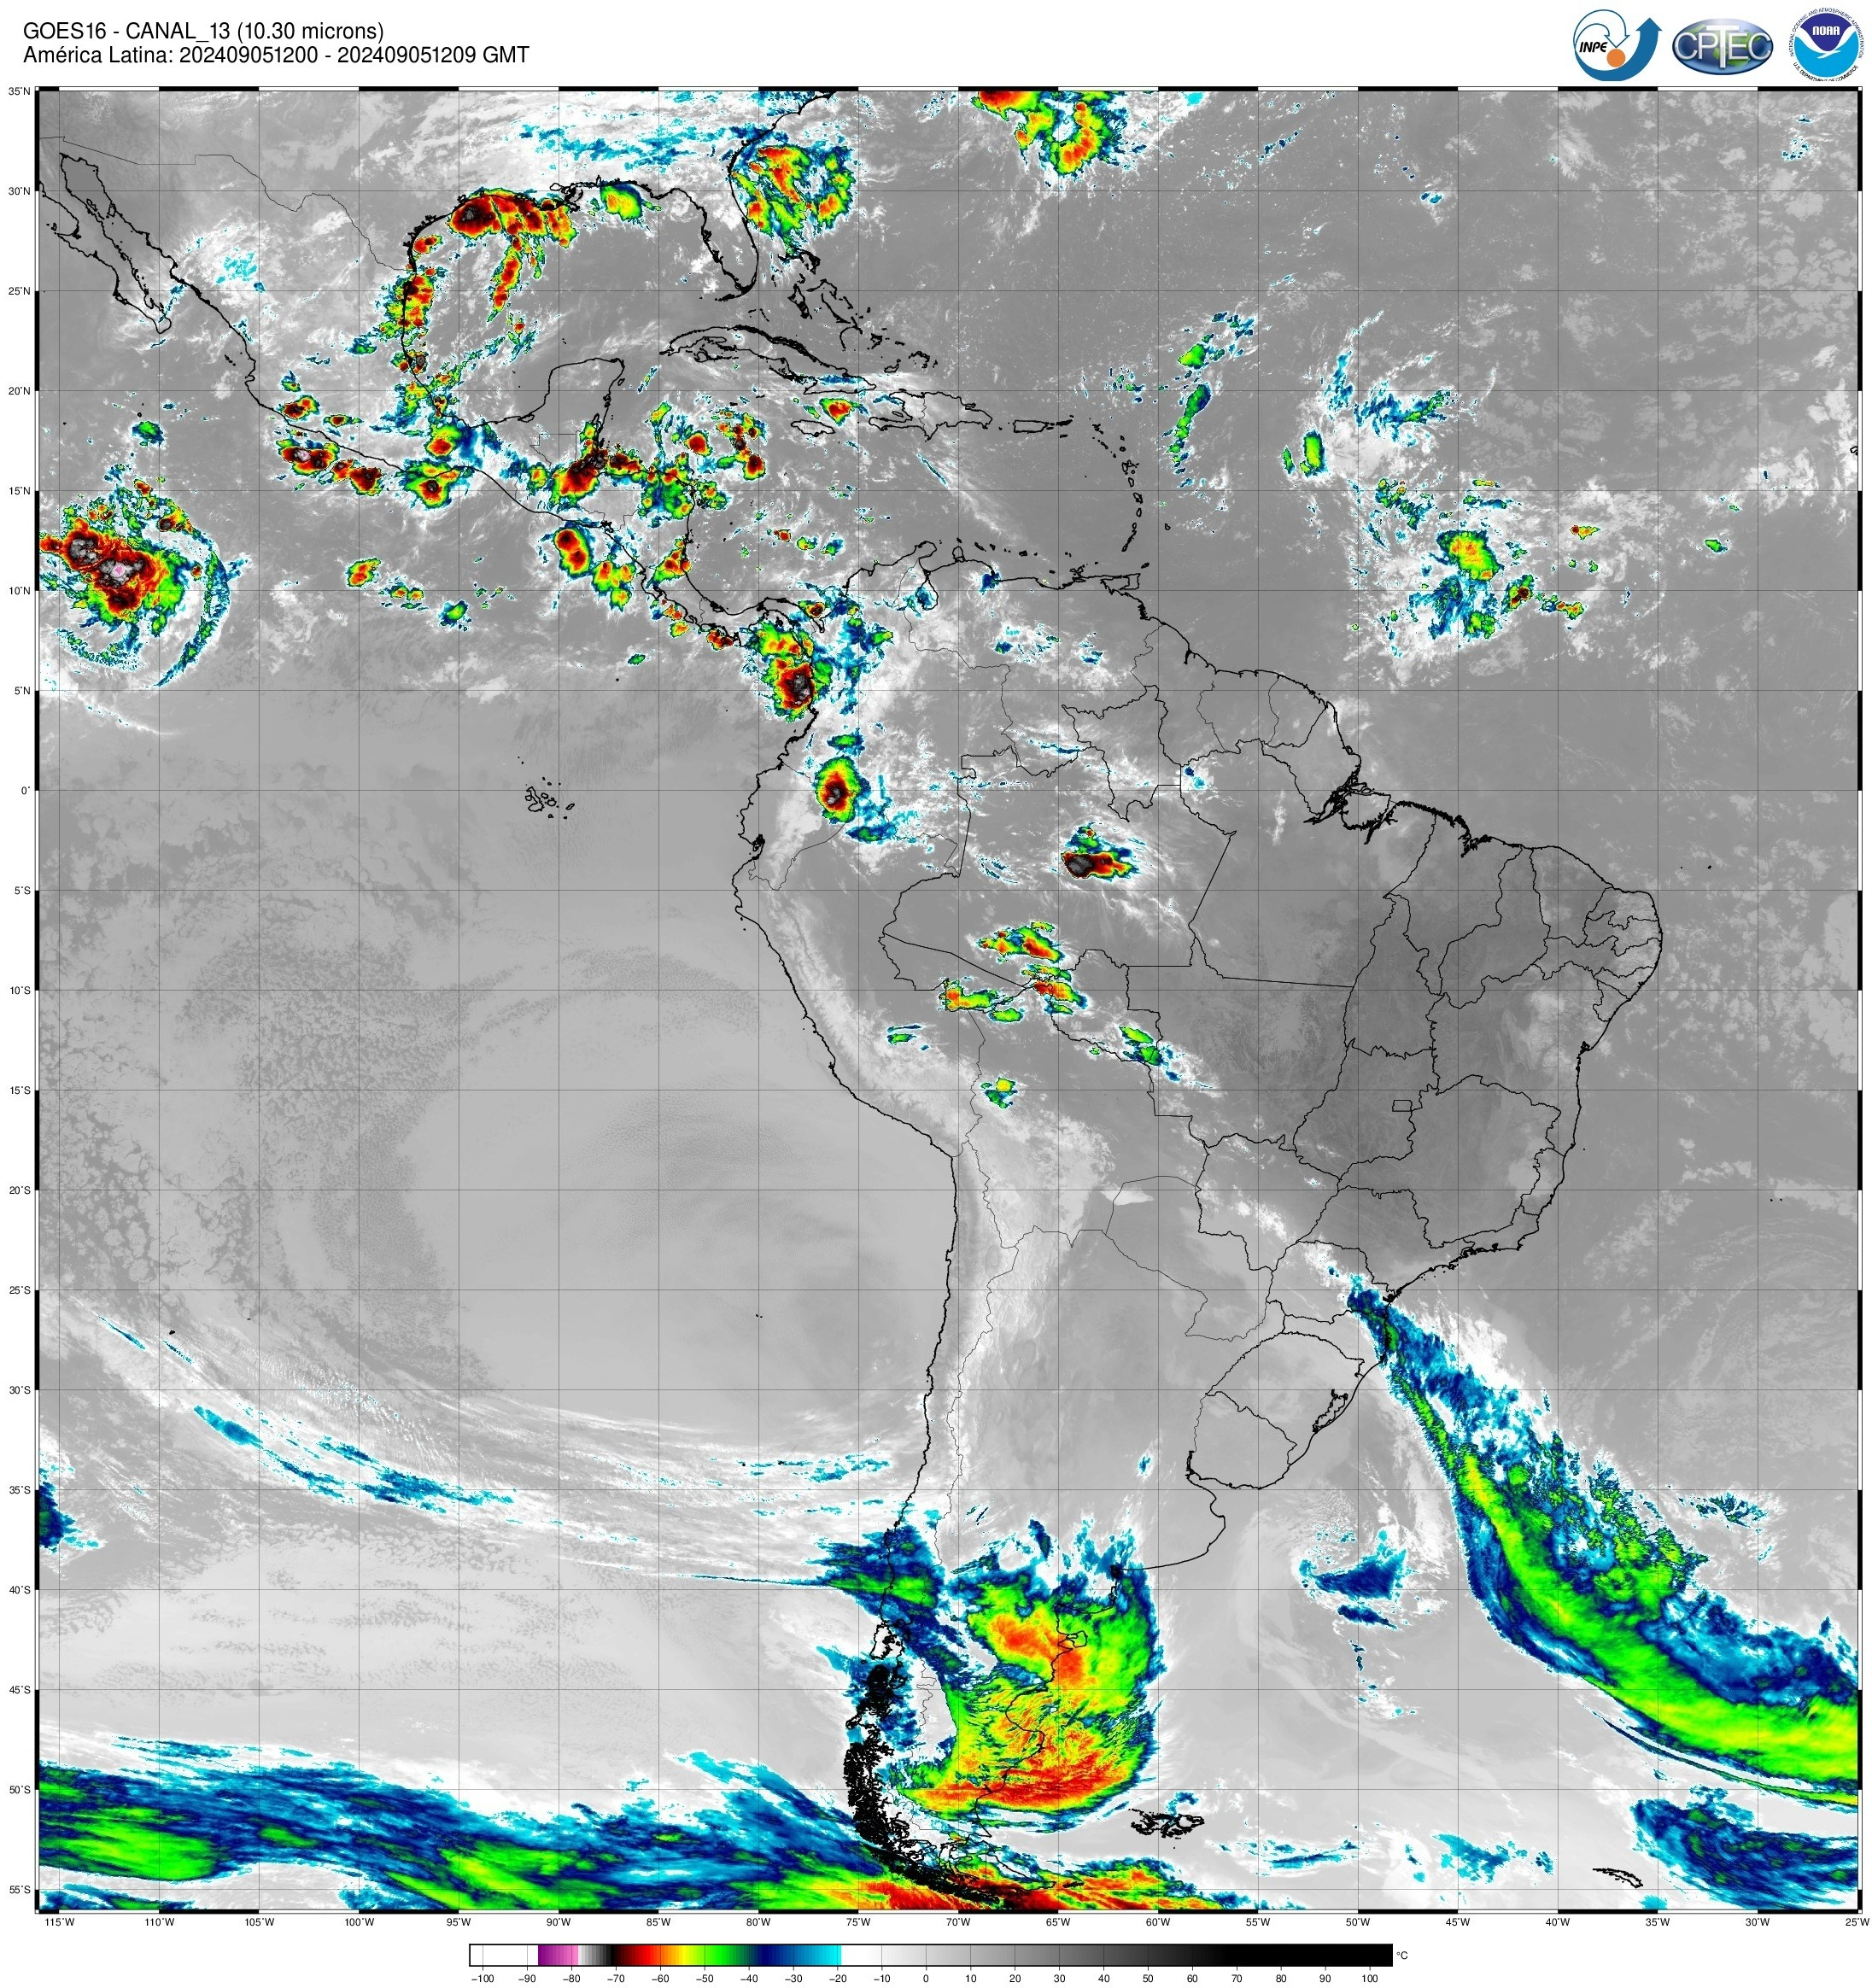
\includegraphics[width=\textwidth, trim=0cm 0cm 0cm 3.5cm, clip]{images/goes16_ch13_202409051200.jpg}
	\caption{2024-09-05T12:00}
	\label{fig:goes16_ch13_202409051200}
	\end{subfigure}
	\hfill
	\begin{subfigure}[b]{0.4\textwidth}
		\centering
		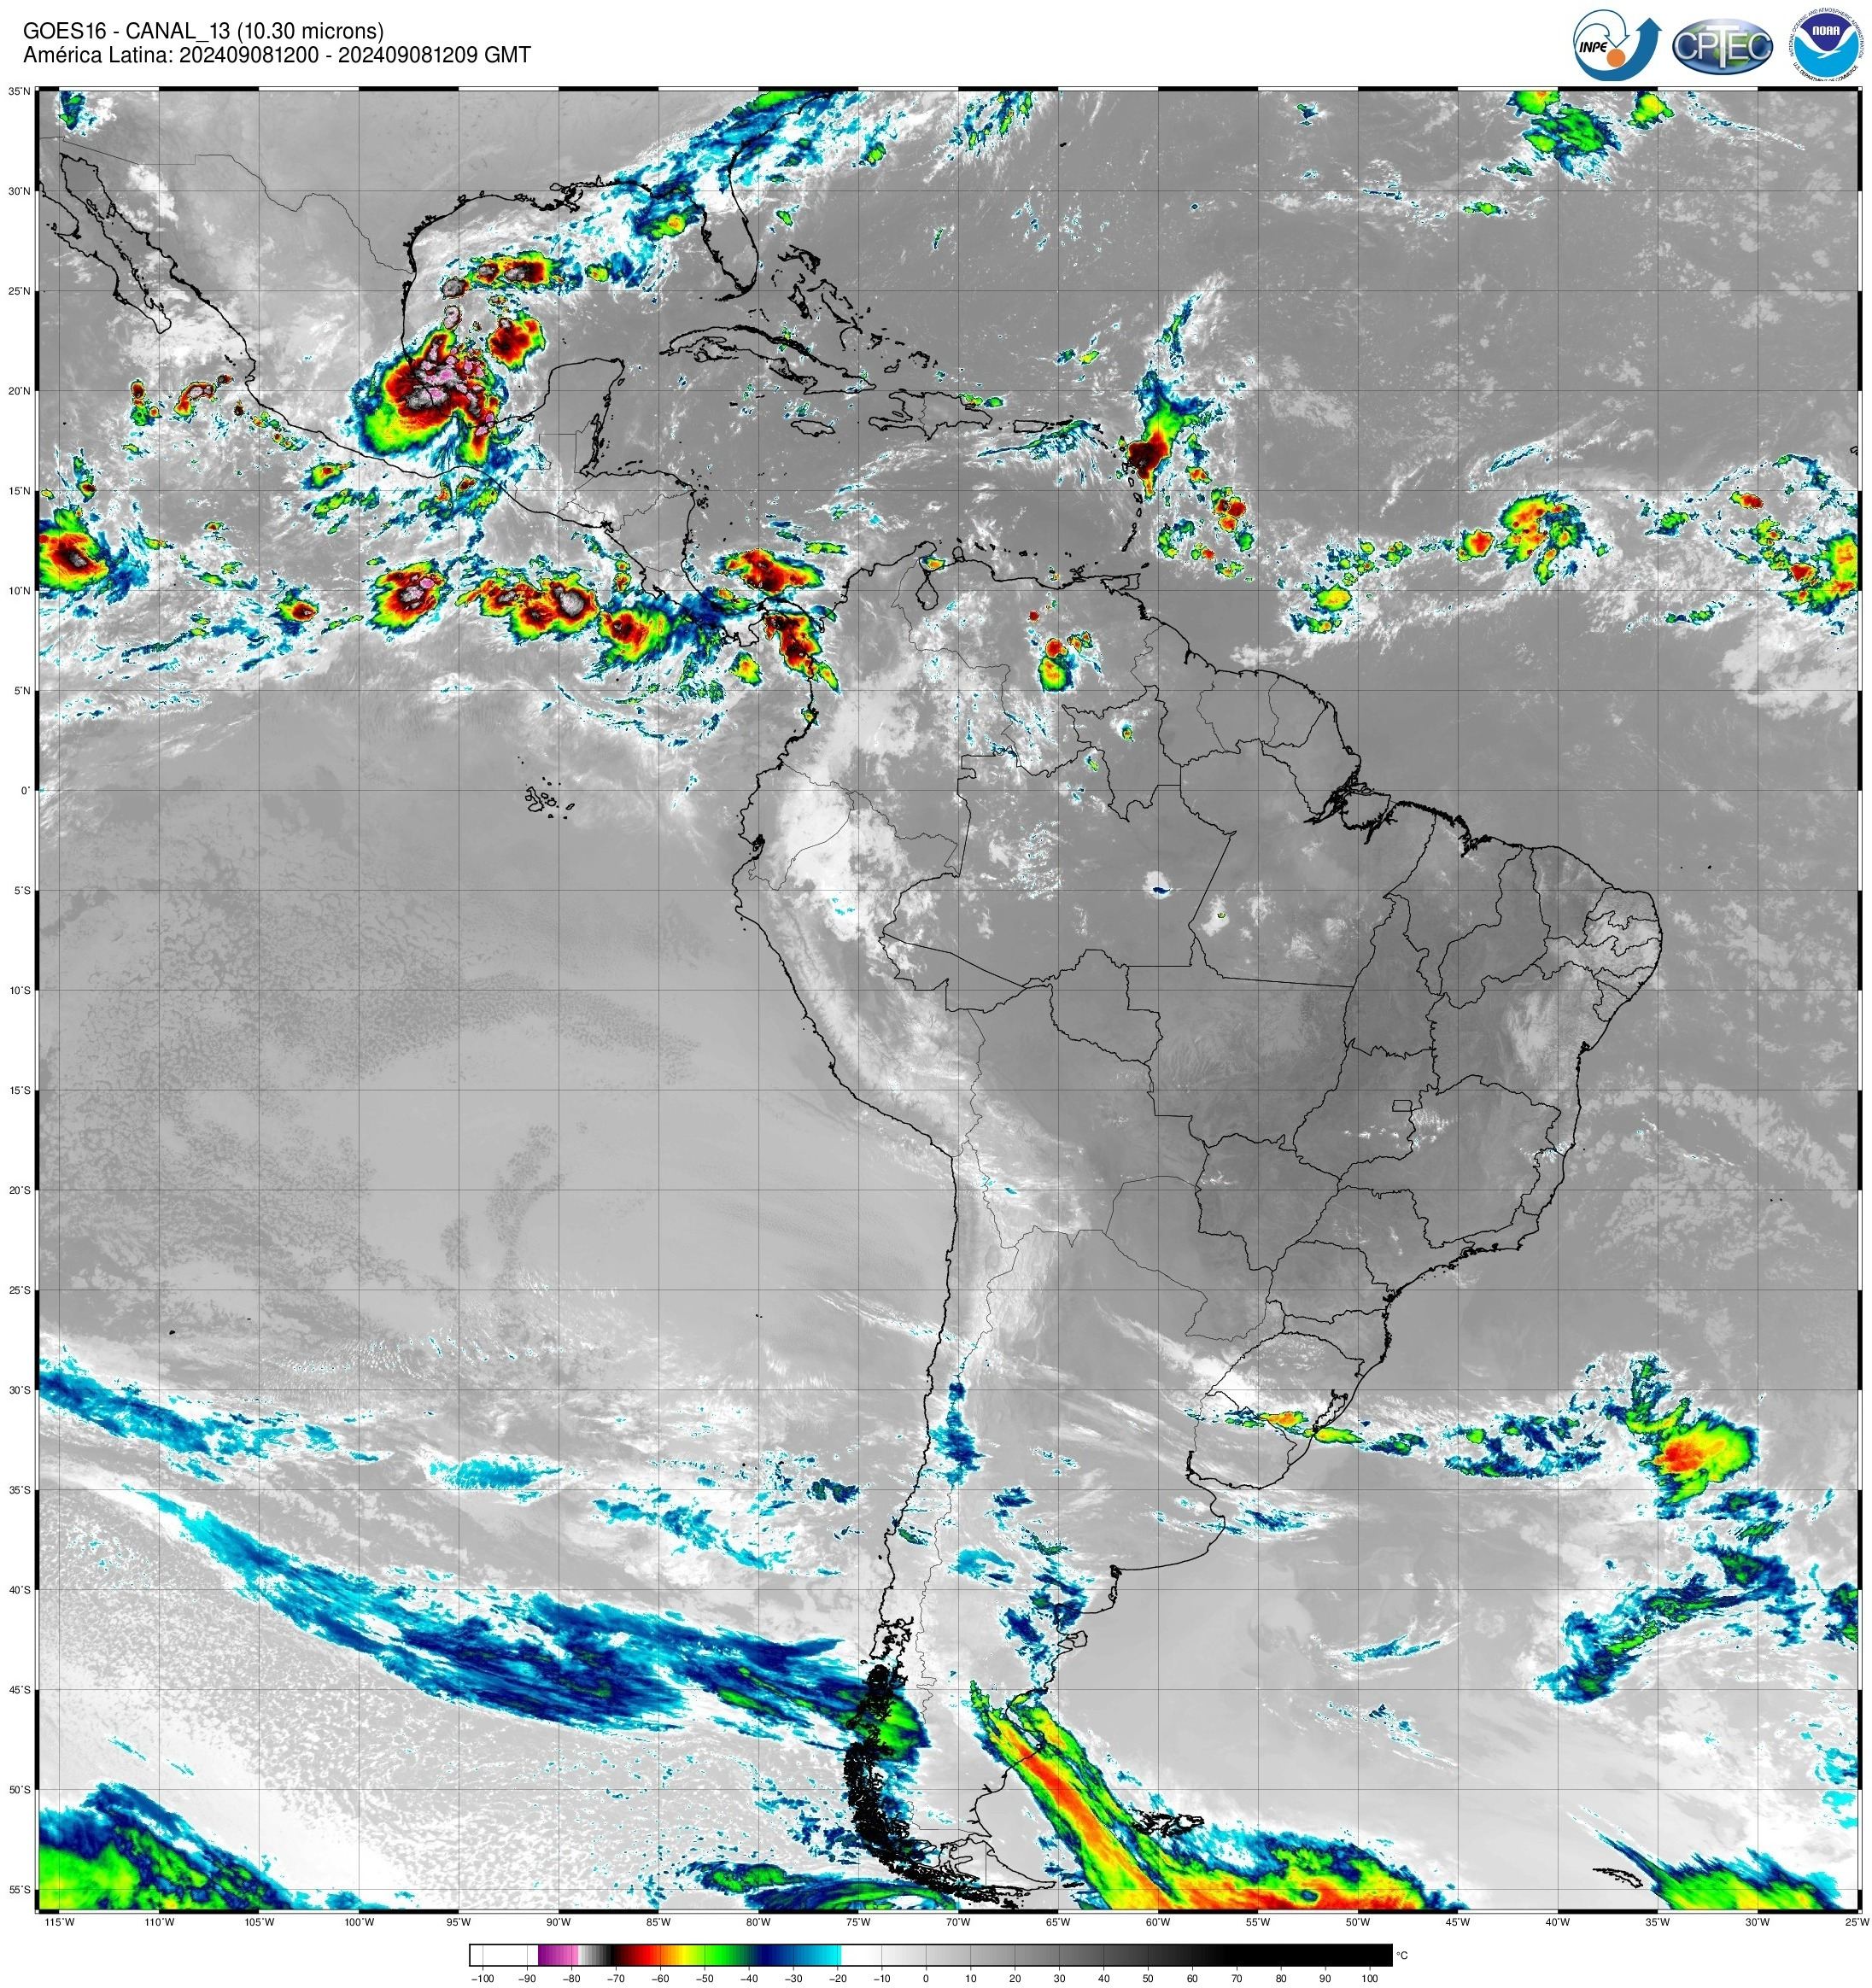
\includegraphics[width=\textwidth, trim=0cm 0cm 0cm 3.5cm, clip]{images/goes16_ch13_202409081200.jpg}
		\caption{2024-09-08T12:00}
		\label{fig:goes16_ch13_202409081200}
	\end{subfigure}
	\hfill
	\begin{subfigure}[b]{0.4\textwidth}
		\centering
		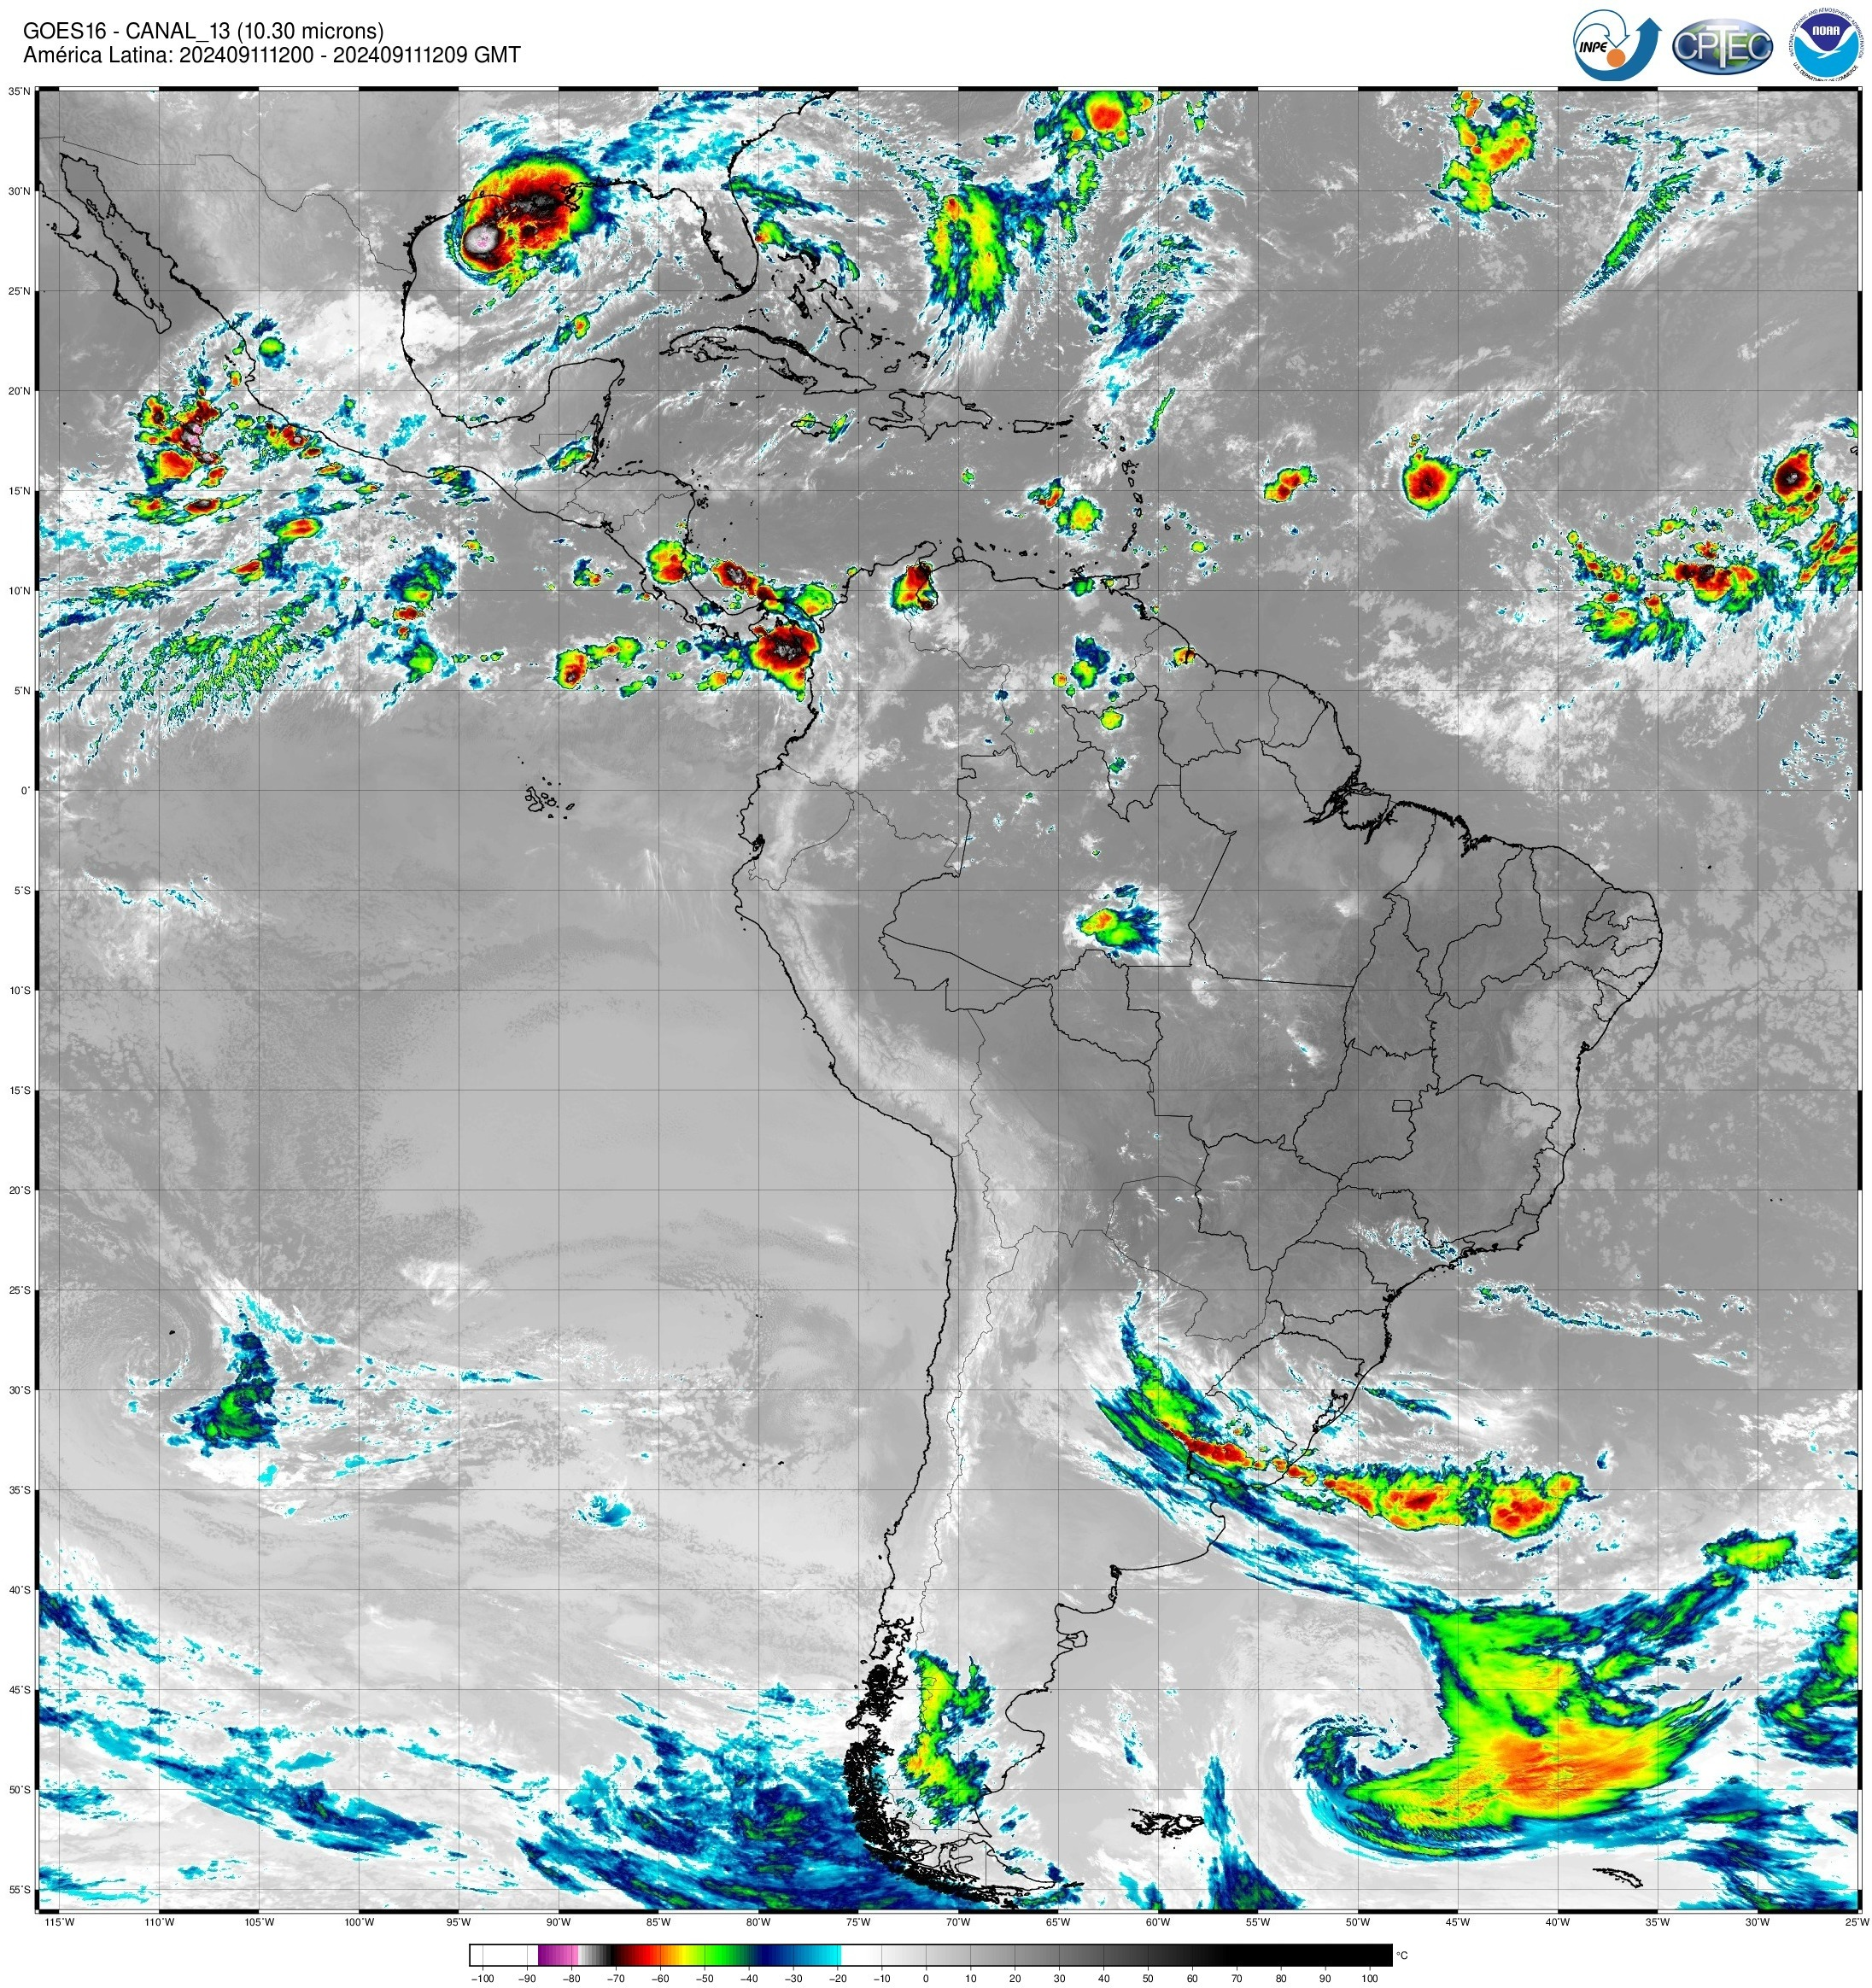
\includegraphics[width=\textwidth, trim=0cm 0cm 0cm 3.5cm, clip]{images/goes16_ch13_202409111200.jpg}
		\caption{2024-09-11T12:00}
		\label{fig:goes16_ch13_202409111200}
	\end{subfigure}
	\hfill
	\begin{subfigure}[b]{0.4\textwidth}
		\centering
		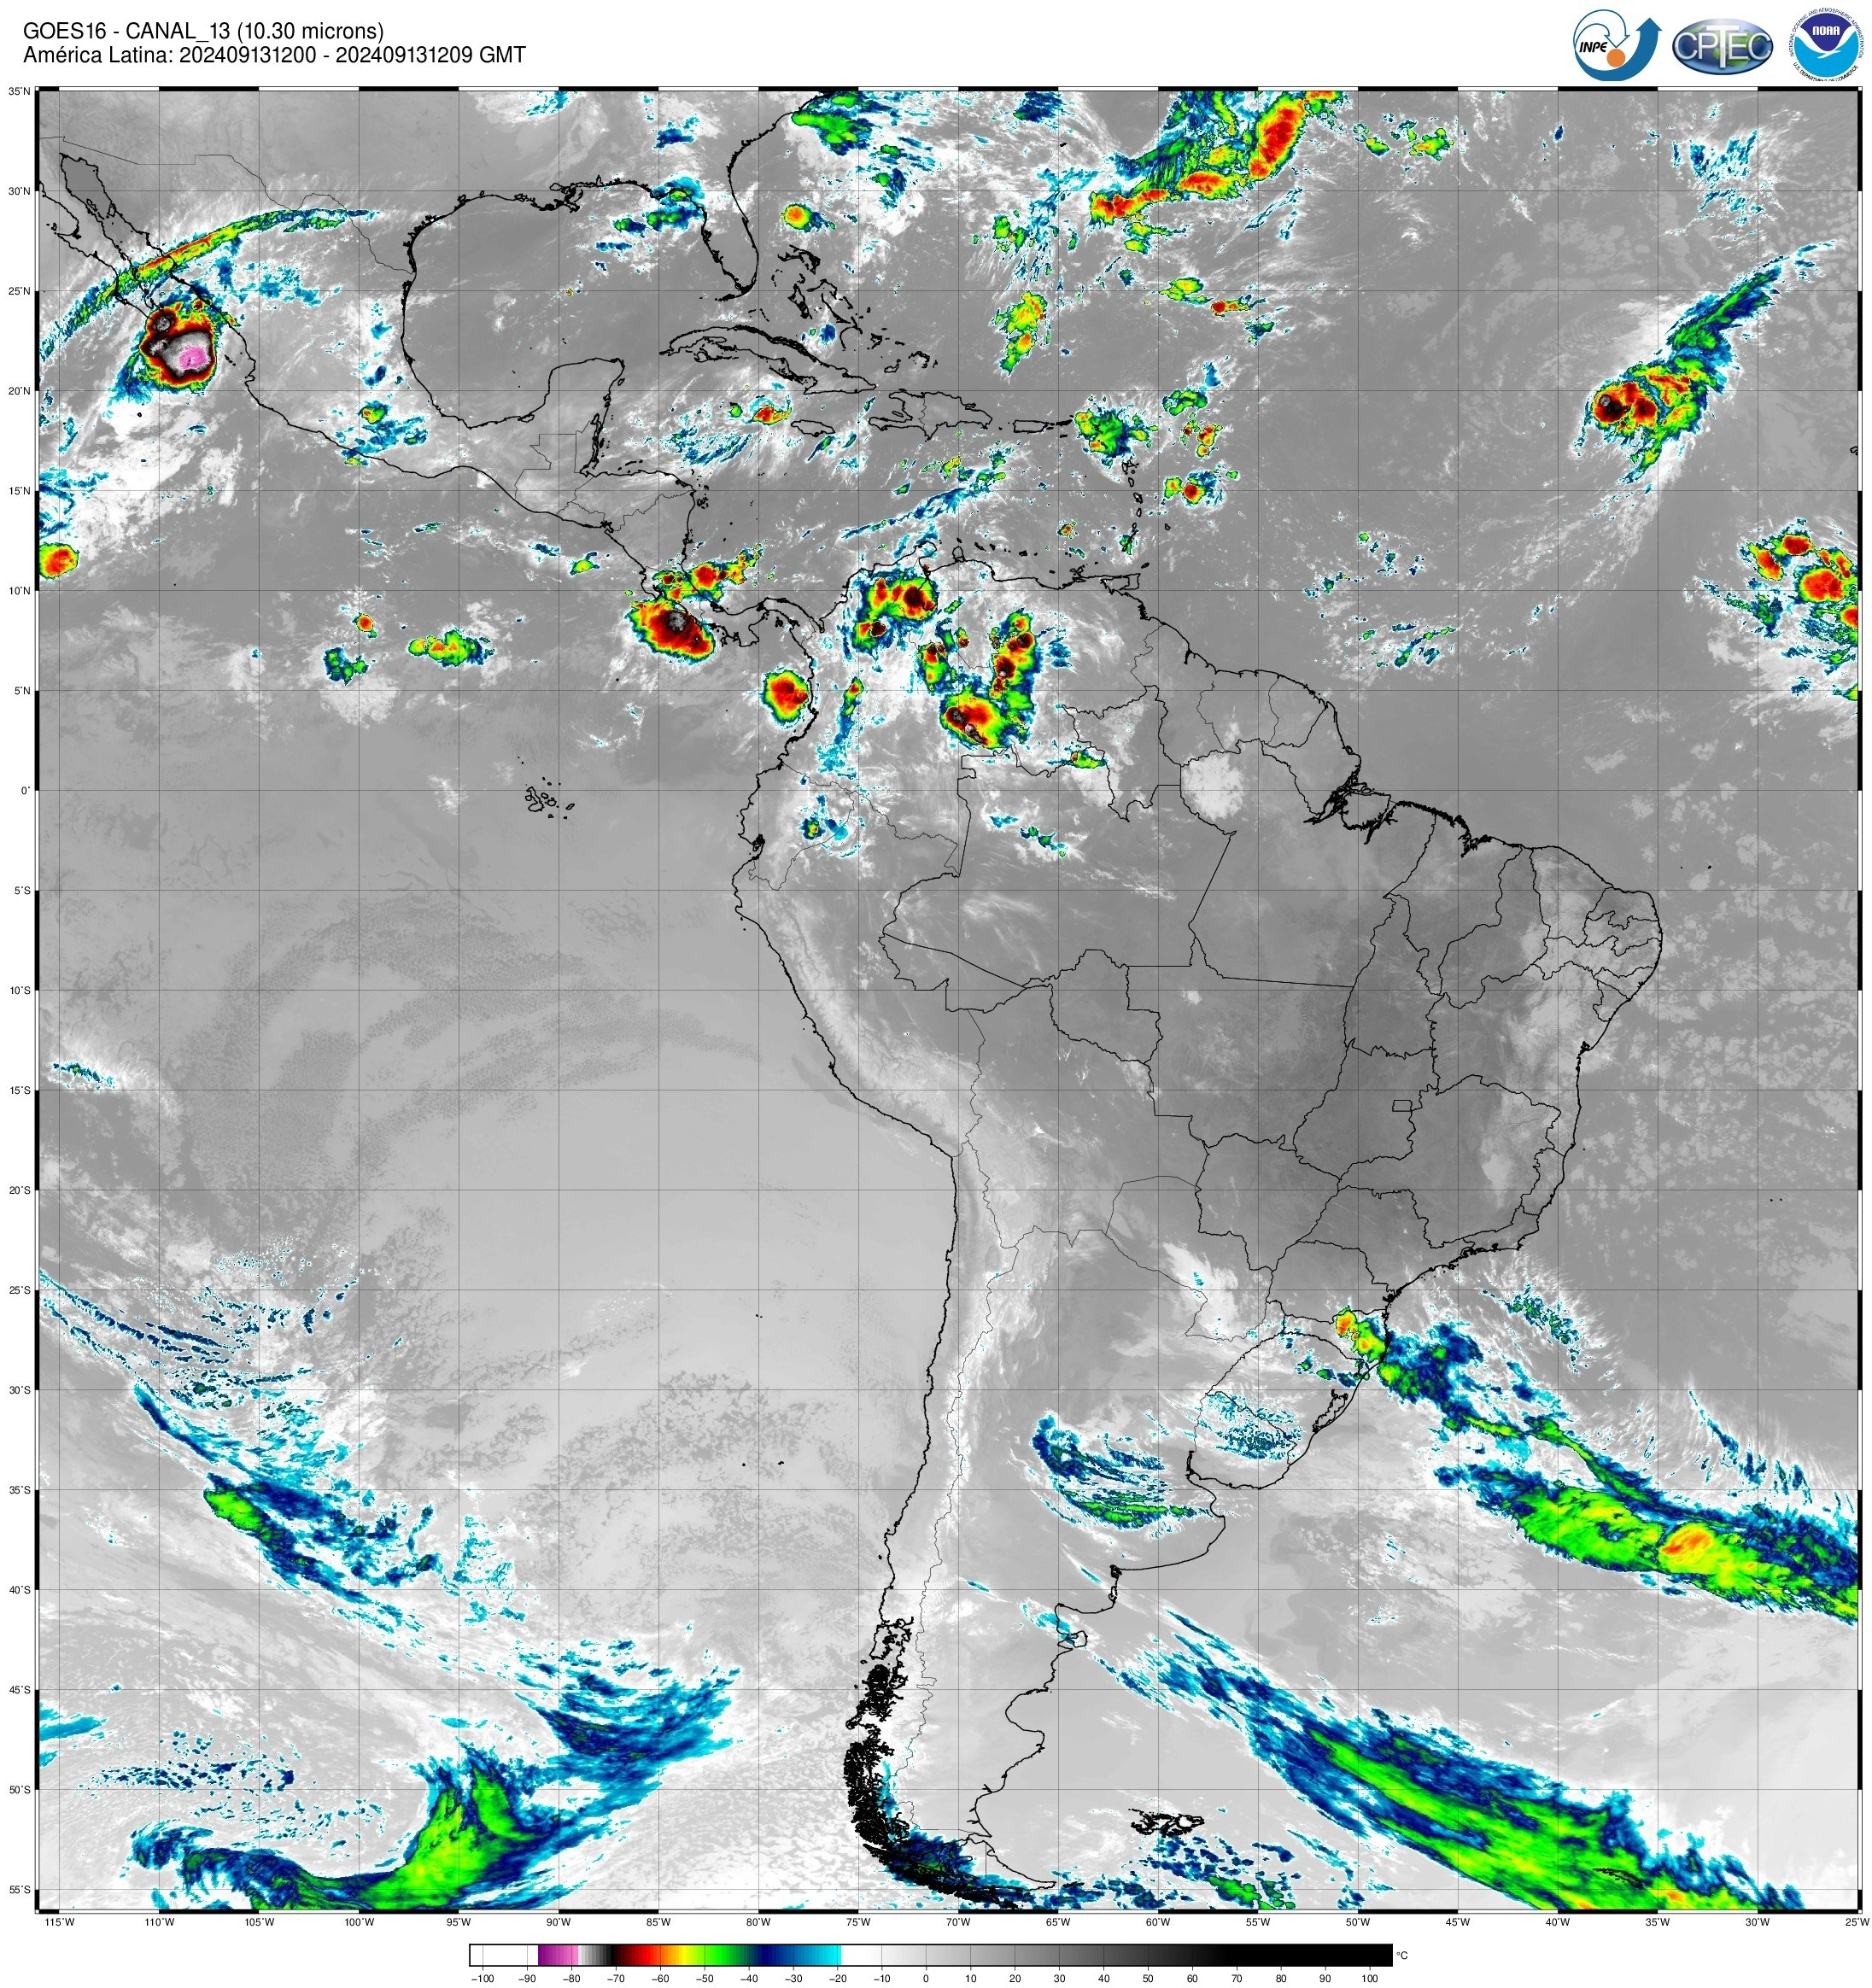
\includegraphics[width=\textwidth, trim=0cm 0cm 0cm 3.5cm, clip]{images/goes16_ch13_202409131200.jpg}
		\caption{2024-09-13T12:00}
		\label{fig:goes16_ch13_202409131200}
	\end{subfigure}
	\caption{Imagens do satélite GOES16 no canal 13 para entre os dias 05 e 13 de setembro de 2024}
	\label{fig:goesgeral}	
\end{figure}




Com o objetivo de analisar as condições da circulação atmosférica que podem ter contribuído para o aumento da concentração de aerossóis, como o black carbon (BC), sobre Santa Catarina, foram analisados os campos de vento em 750, 800 e 850 hPa para os dias 11, 12 e 13 de setembro, conforme apresentado na Figura 8. Os resultados evidenciam um padrão de circulação atmosférica associado ao South American Low-Level Jet (SALLJ), com escoamento direcionado para a região Sul do Brasil, em concordância com as análises preliminares apresentadas por \autocite{forgioni2025}.
Esses resultados sugerem que a circulação atmosférica favoreceu o transporte de aerossóis para Santa Catarina, contribuindo para o aumento dos valores de AOD observados no estado, especialmente na região Oeste, que constitui a primeira área do estado impactada pelo transporte dessas partículas. 




\begin{figure}[htbp]
	\centering
	% --- LINHA 1 ---
	\begin{subfigure}[b]{0.31\textwidth}
		\centering
		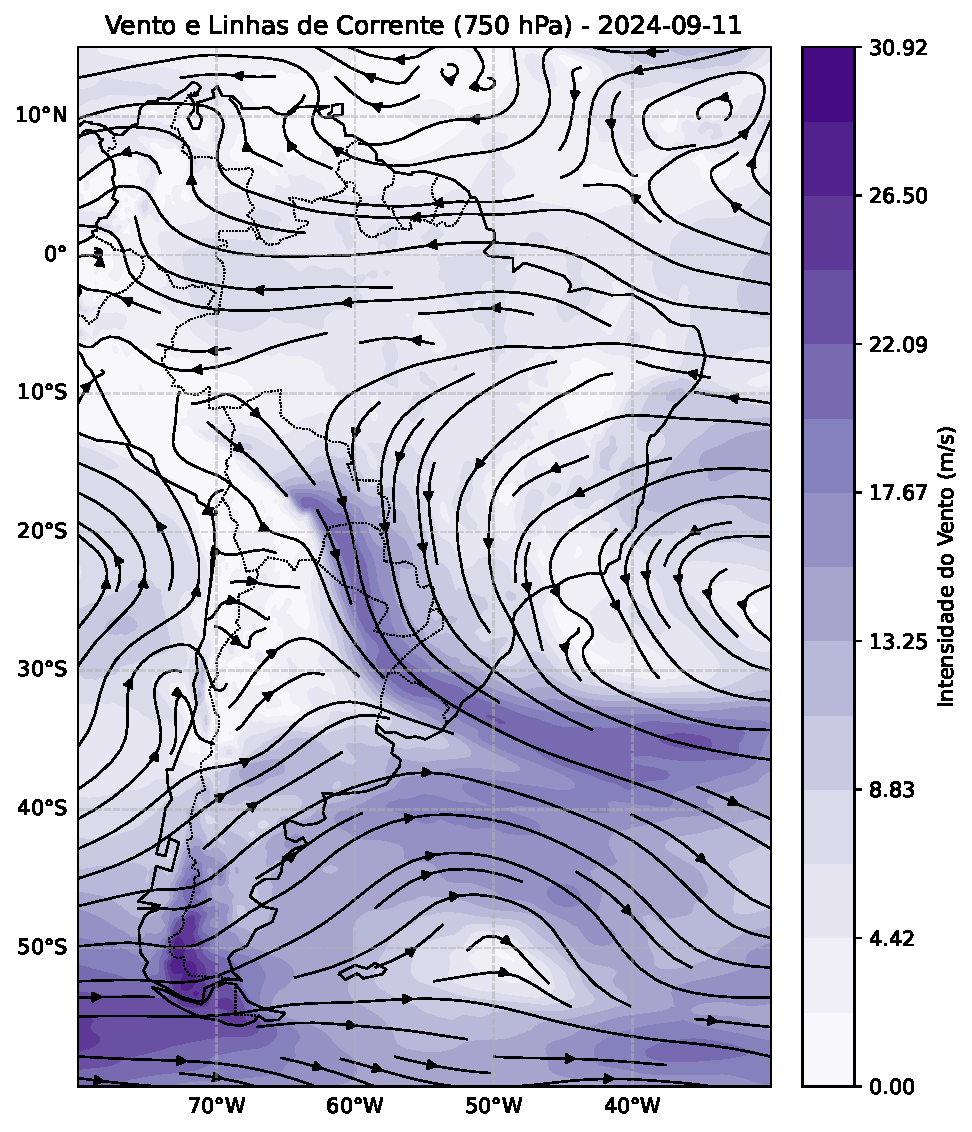
\includegraphics[width=\textwidth, trim=0cm 0cm 0cm 0.6cm, clip]{images/vento_750hPa_2024-09-11.pdf}
		\caption{750hPa 2024-09-11}
		\label{fig:img1}
	\end{subfigure}
	\hfill
	\begin{subfigure}[b]{0.31\textwidth}
		\centering
		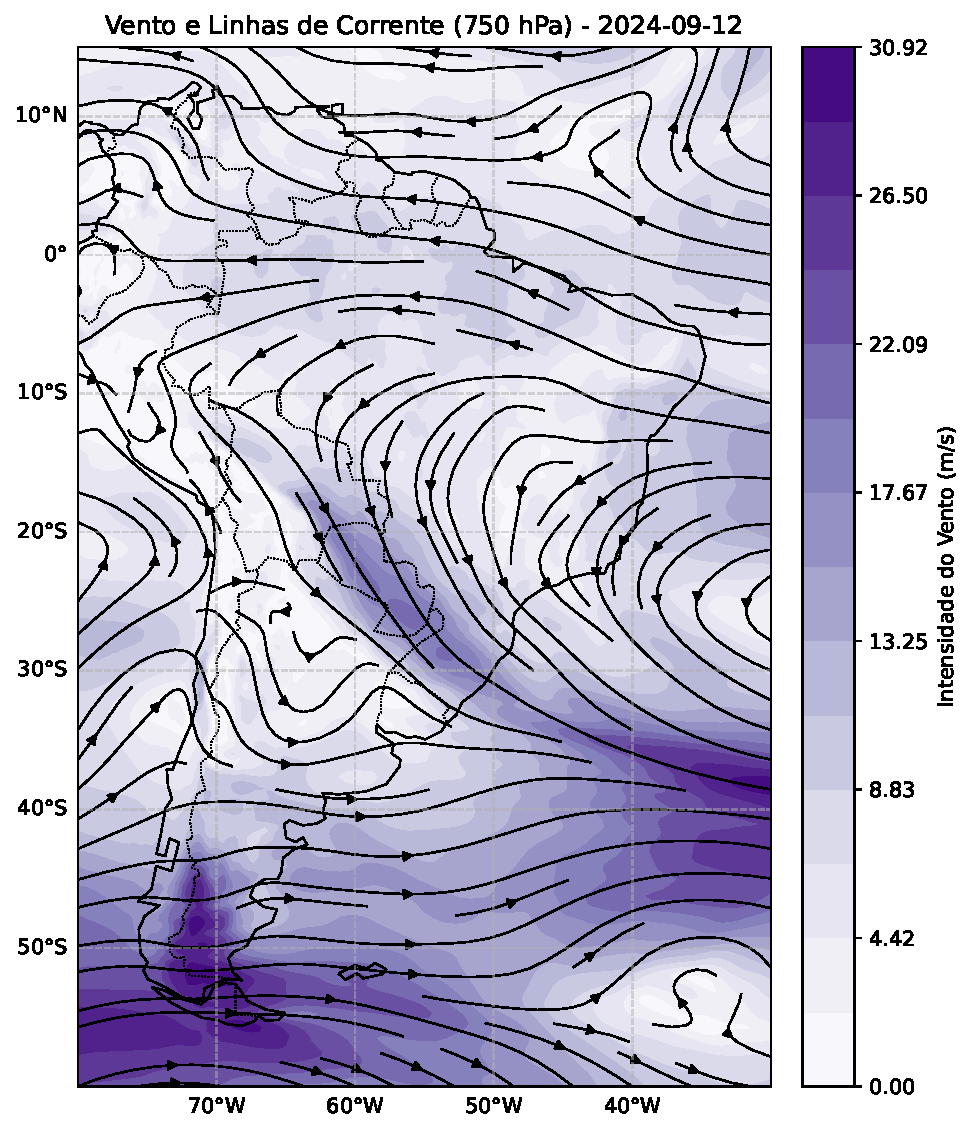
\includegraphics[width=\textwidth, trim=0cm 0cm 0cm 0.6cm, clip]{images/vento_750hPa_2024-09-12.pdf}
		\caption{750hPa 2024-09-12}
		\label{fig:img2}
	\end{subfigure}
	\hfill
	\begin{subfigure}[b]{0.31\textwidth}
		\centering
		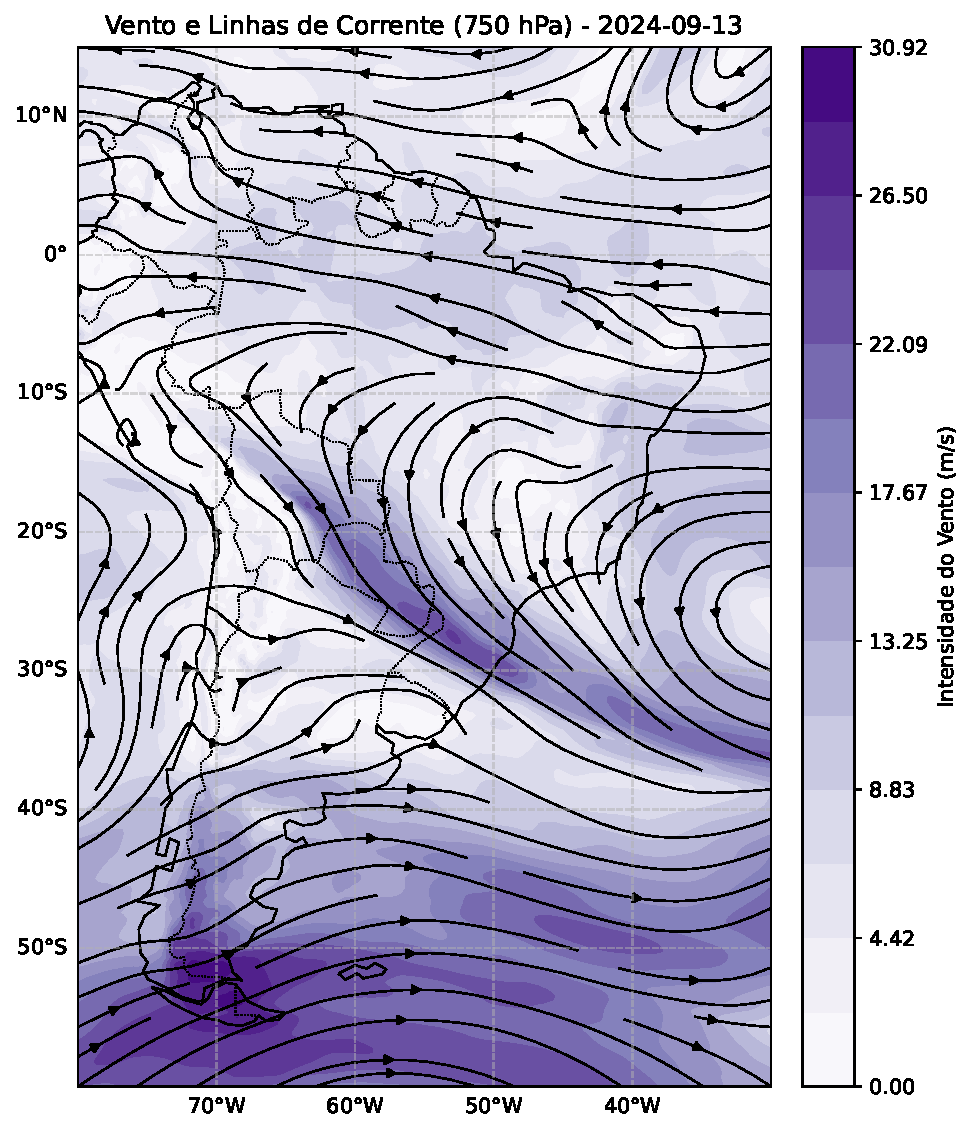
\includegraphics[width=\textwidth, trim=0cm 0cm 0cm 0.6cm, clip]{images/vento_750hPa_2024-09-13.pdf}
		\caption{750hPa 2024-09-13}
		\label{fig:img3}
	\end{subfigure}
	
	\vspace{0.8em} % Espaçamento vertical entre as linhas
	
	% --- LINHA 2 ---
	\begin{subfigure}[b]{0.31\textwidth}
		\centering
		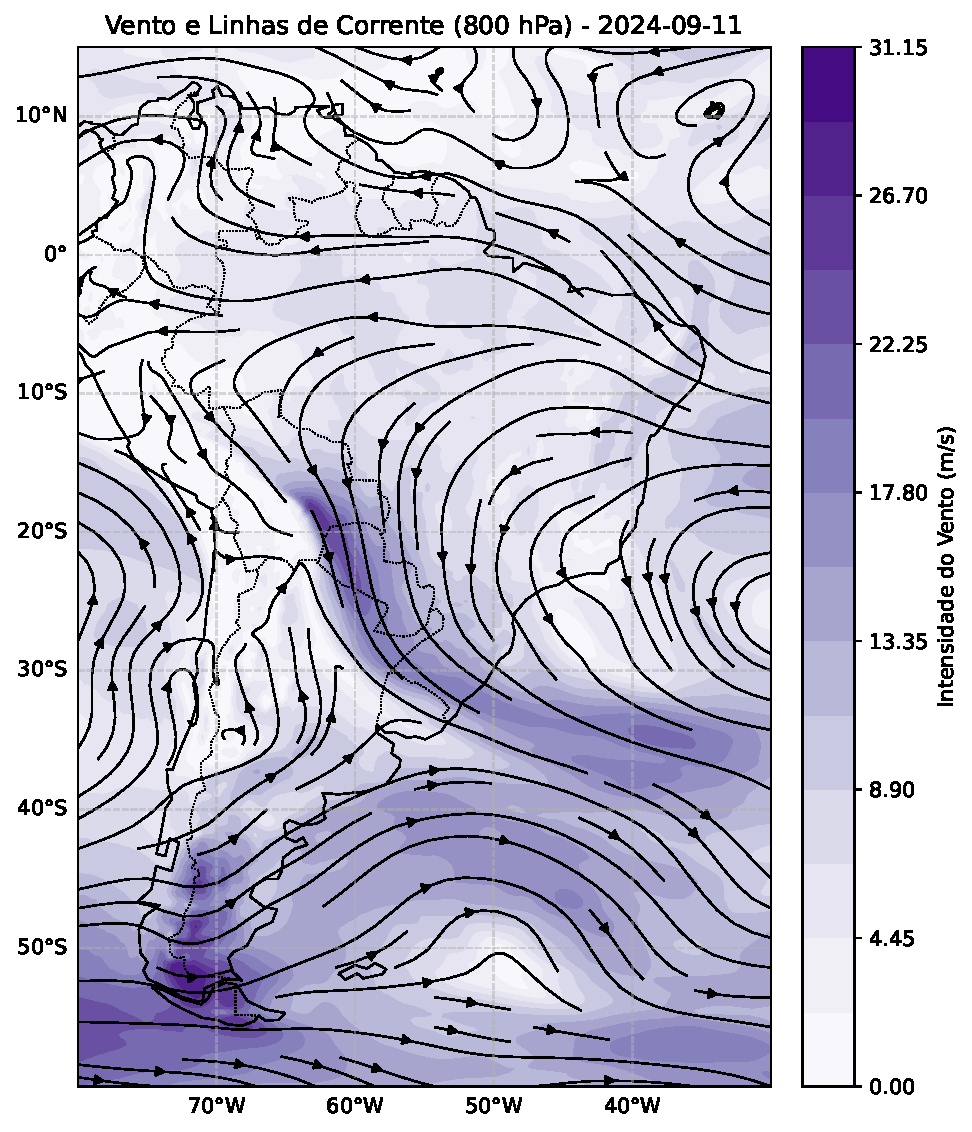
\includegraphics[width=\textwidth, trim=0cm 0cm 0cm 0.6cm, clip]{images/vento_800hPa_2024-09-11.pdf}
		\caption{800hPa 2024-09-11}
		\label{fig:img4}
	\end{subfigure}
	\hfill
	\begin{subfigure}[b]{0.31\textwidth}
		\centering
		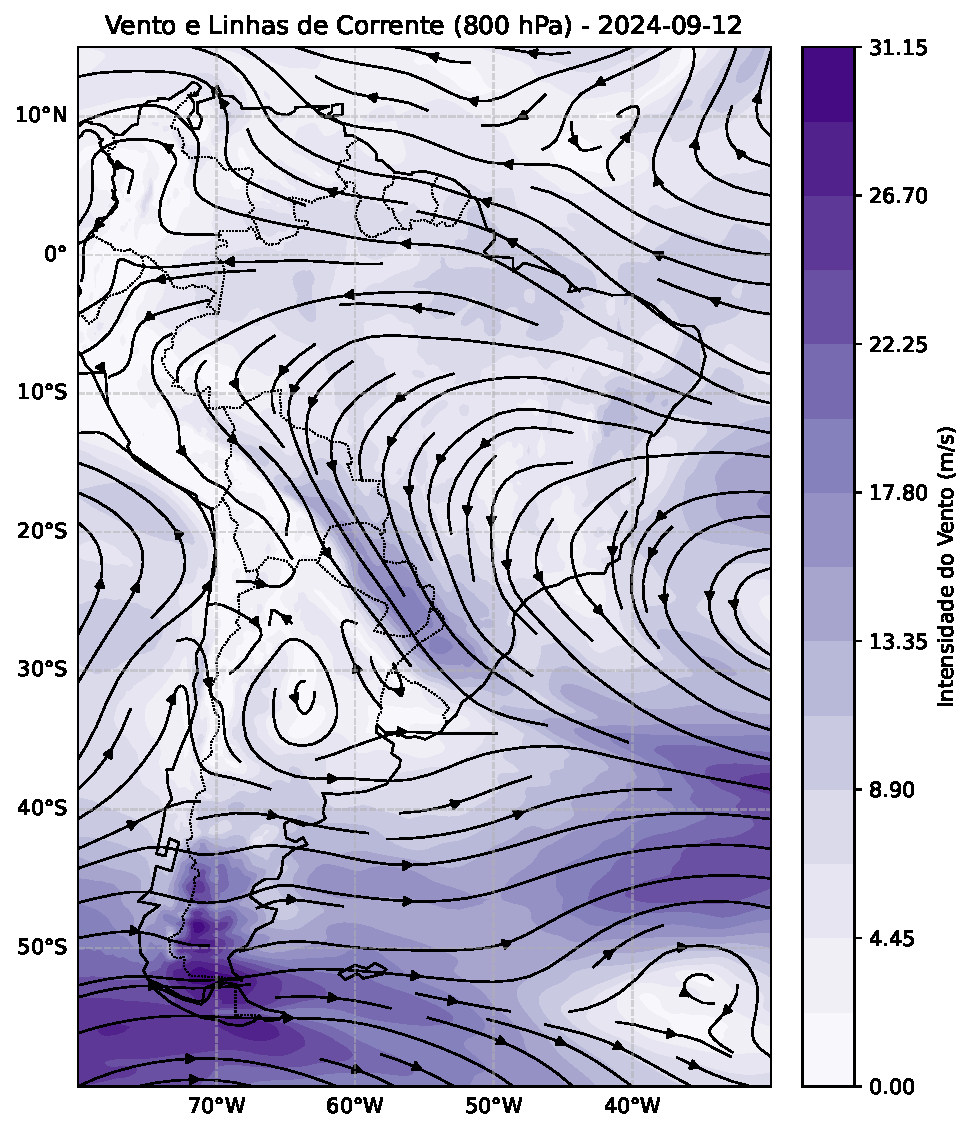
\includegraphics[width=\textwidth, trim=0cm 0cm 0cm 0.6cm, clip]{images/vento_800hPa_2024-09-12.pdf}
		\caption{800hPa 2024-09-12}
		\label{fig:img5}
	\end{subfigure}
	\hfill
	\begin{subfigure}[b]{0.31\textwidth}
		\centering
		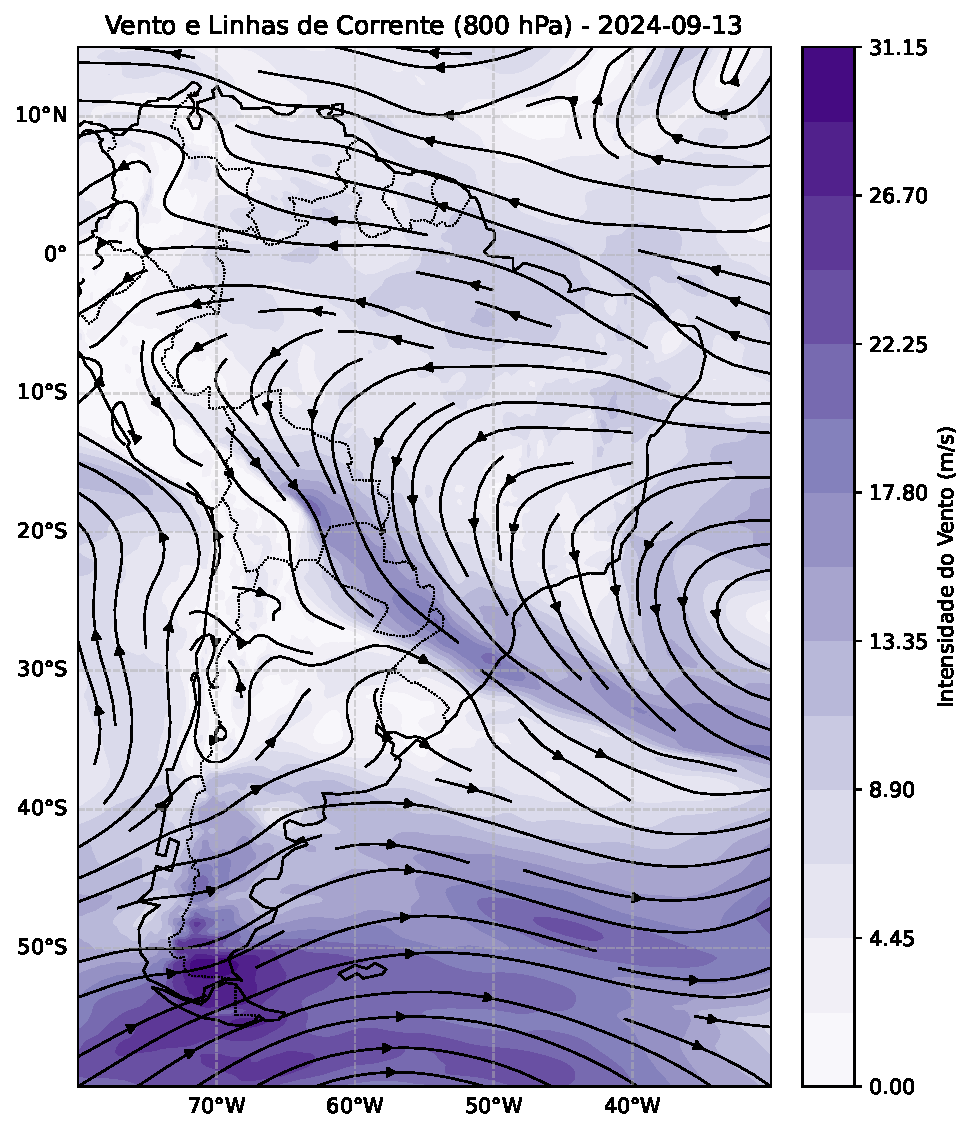
\includegraphics[width=\textwidth, trim=0cm 0cm 0cm 0.6cm, clip]{images/vento_800hPa_2024-09-13.pdf}
		\caption{800hPa 2024-09-13}
		\label{fig:img6}
	\end{subfigure}
	
	\vspace{0.8em} % Espaçamento vertical entre as linhas
	
	% --- LINHA 3 ---
	\begin{subfigure}[b]{0.31\textwidth}
		\centering
		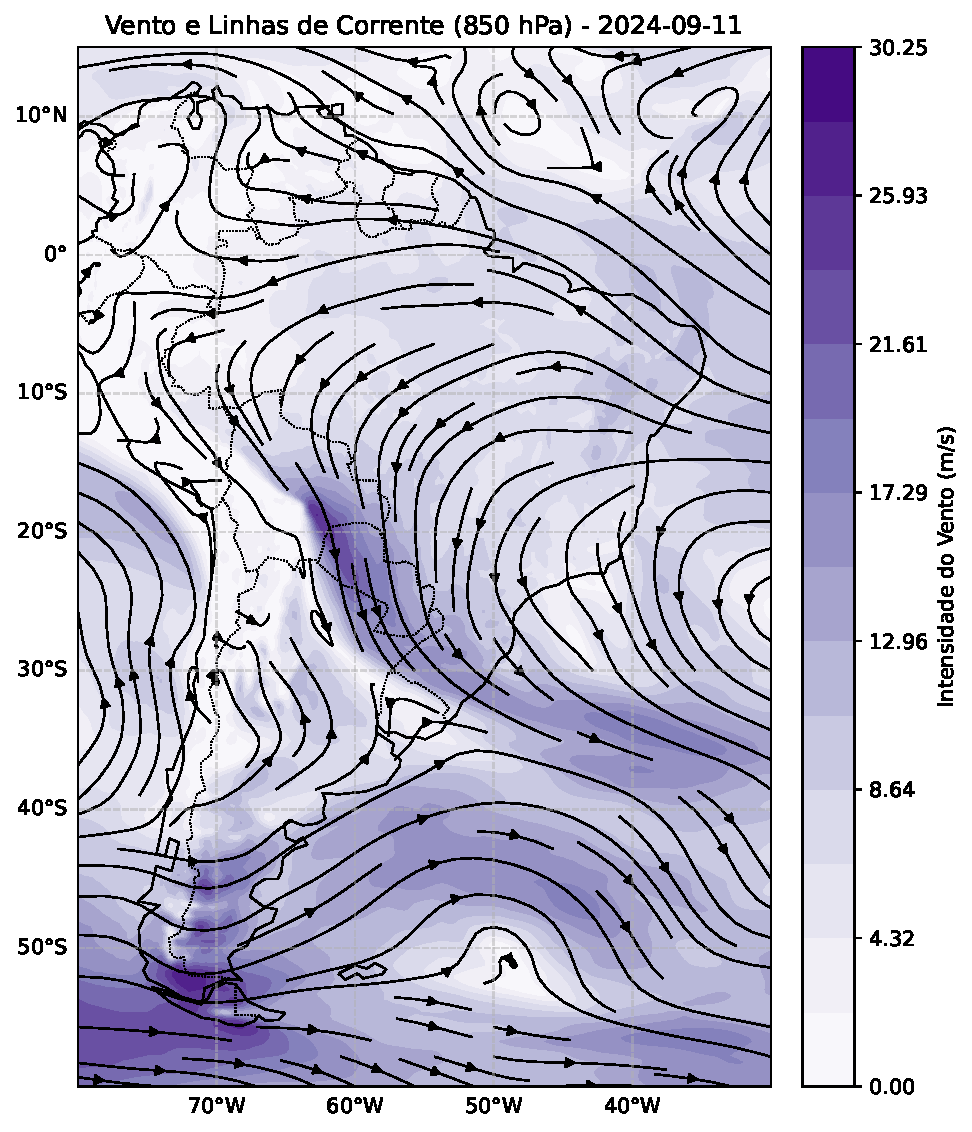
\includegraphics[width=\textwidth, trim=0cm 0cm 0cm 0.6cm, clip]{images/vento_850hPa_2024-09-11.pdf}
		\caption{850hPa 2024-09-11}
		\label{fig:img7}
	\end{subfigure}
	\hfill
	\begin{subfigure}[b]{0.31\textwidth}
		\centering
		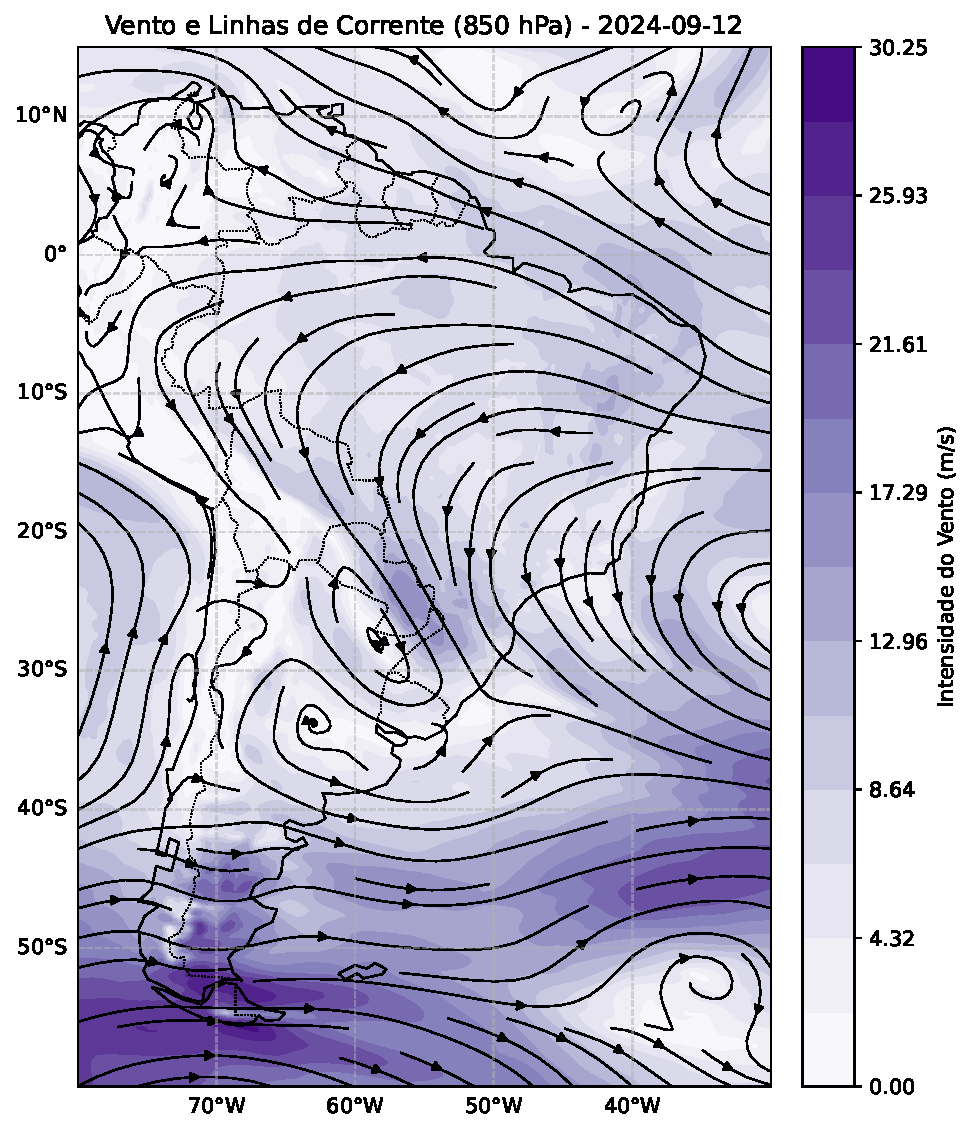
\includegraphics[width=\textwidth,
		trim=0cm 0cm 0cm 0.6cm, clip]{images/vento_850hPa_2024-09-12.pdf}
		\caption{850hPa 2024-09-12}
		\label{fig:img8}
	\end{subfigure}
	\hfill
	\begin{subfigure}[b]{0.31\textwidth}
		\centering
		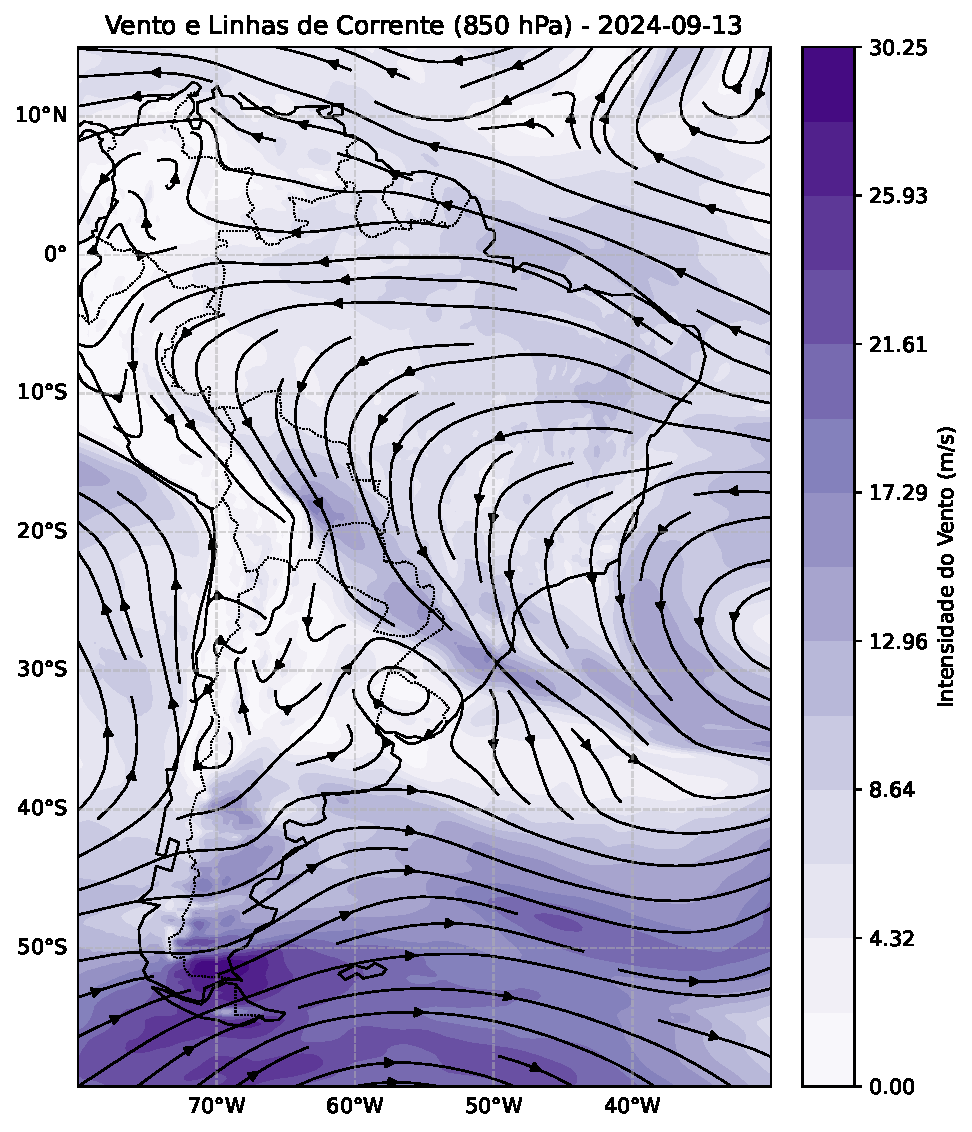
\includegraphics[width=\textwidth, trim=0cm 0cm 0cm 0.6cm, clip]{images/vento_850hPa_2024-09-13.pdf}
		\caption{850hPa 2024-09-13}
		\label{fig:img9}
	\end{subfigure}
	
	\caption{Médias diárias de direção e intensidade do vento.}
	\label{fig:grade_completa}
\end{figure}


\begin{figure}[htbp]
	\centering
	% --- LINHA 1 ---
	\begin{subfigure}[b]{0.31\textwidth}
		\centering
		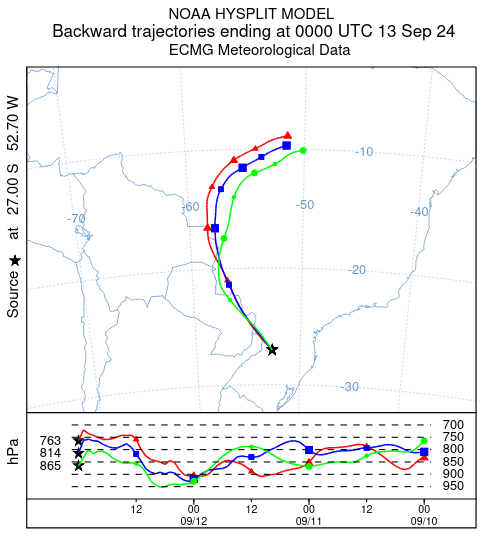
\includegraphics[width=\textwidth, trim=0cm 0cm 0cm 2.1cm, clip]{images/chapeco_traj.png}
		\caption{Chapecó, SC}
		\label{fig:img42}
	\end{subfigure}
	\hfill
	\begin{subfigure}[b]{0.31\textwidth}
		\centering
		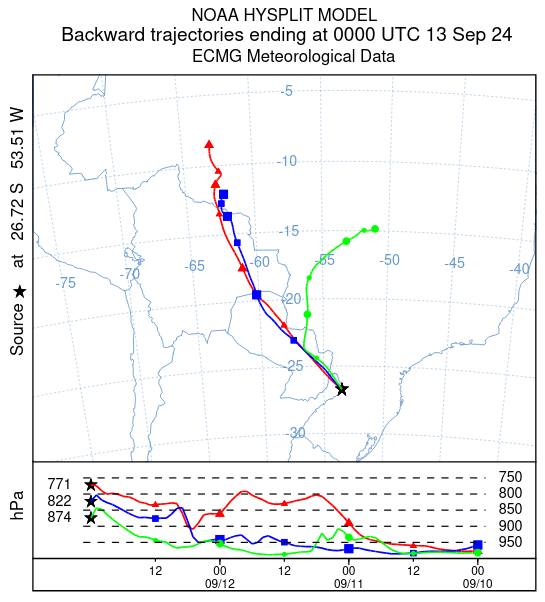
\includegraphics[width=\textwidth, trim=0cm 0cm 0cm 2.3cm, clip]{images/saomiguel_traj.png}
		\caption{São Miguel do Oeste, SC}
		\label{fig:img43}
	\end{subfigure}
	\hfill
	\begin{subfigure}[b]{0.31\textwidth}
		\centering
		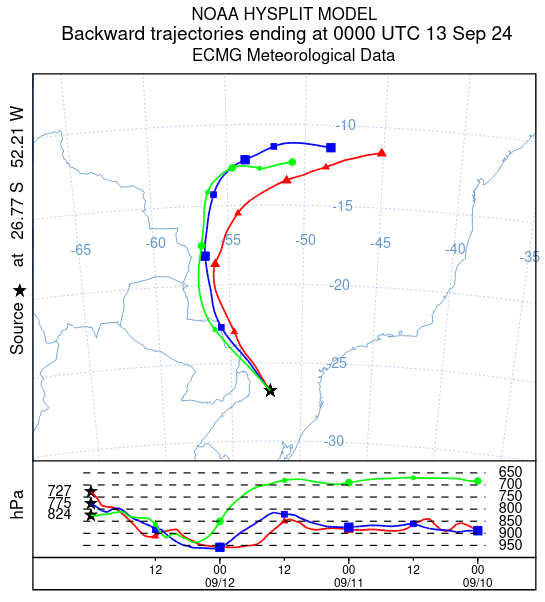
\includegraphics[width=\textwidth, trim=0cm 0cm 0cm 2.3cm, clip]{images/maravilha_traj.png}
		\caption{Maravilha, SC}
		\label{fig:img44}
	\end{subfigure}
	\caption{Trajetórias reversas nos níveis de 750, 800 e 850 hPa entre os dias 09 e 13 de setembro de 2024.}
	\label{fig:traj}
\end{figure}


\begin{figure}[htbp]
	\centering
	% --- LINHA 1 ---
	\begin{subfigure}[b]{0.31\textwidth}
		\centering
		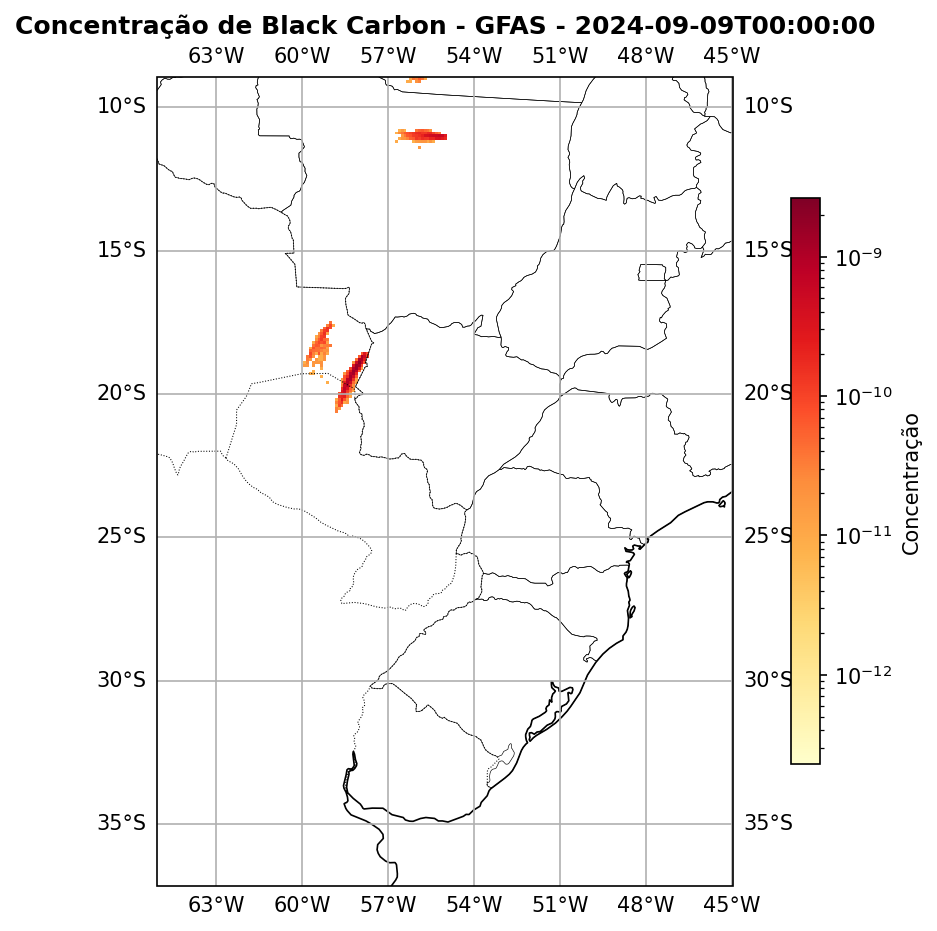
\includegraphics[width=\textwidth, trim=0cm 0cm 0cm 0.7cm, clip]{images/bc_000.png}
		\caption{2024-09-09 00:00:00}
		\label{fig:img10}
	\end{subfigure}
	\hfill
	\begin{subfigure}[b]{0.31\textwidth}
		\centering
		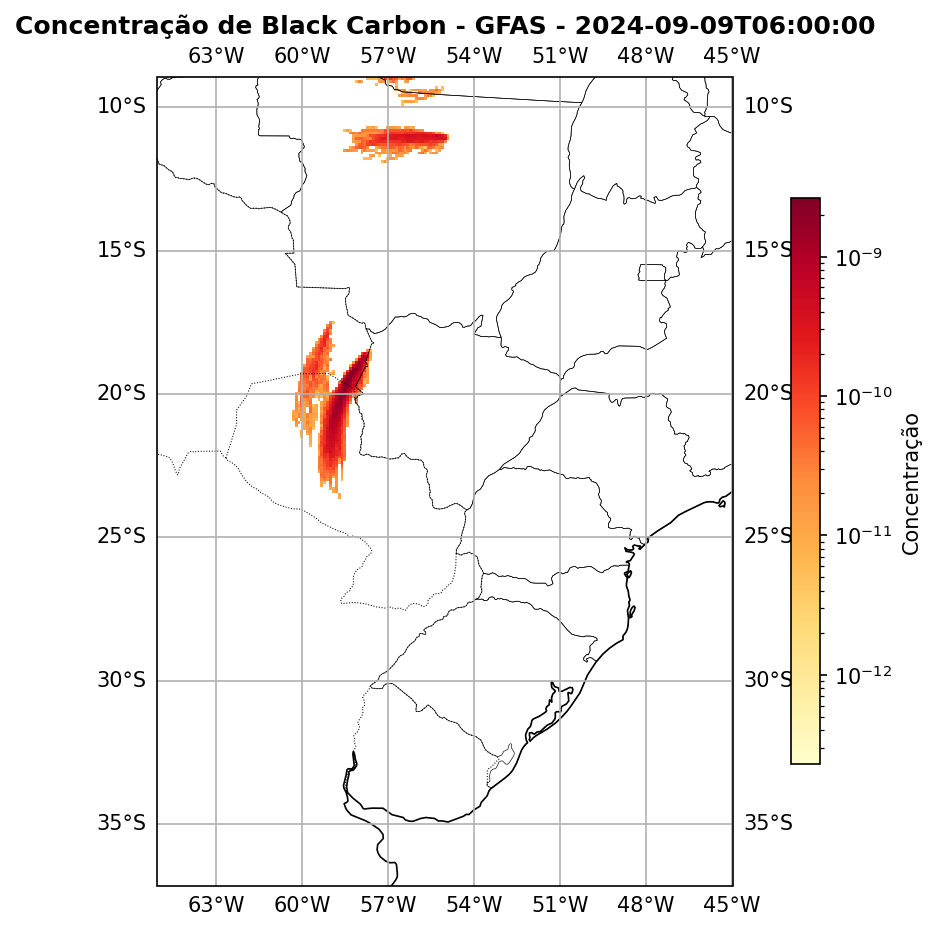
\includegraphics[width=\textwidth, trim=0cm 0cm 0cm 0.7cm, clip]{images/bc_001.png}
		\caption{2024-09-09 00:06:00}
		\label{fig:img11}
	\end{subfigure}
	\hfill
	\begin{subfigure}[b]{0.31\textwidth}
		\centering
		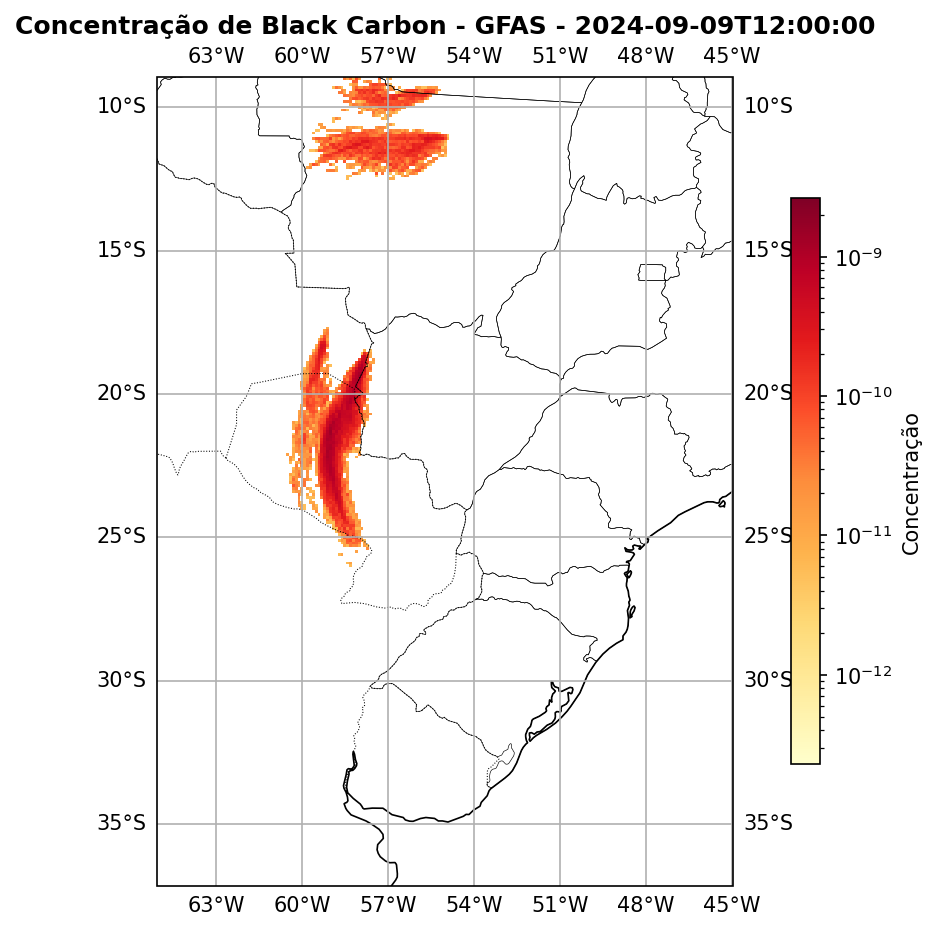
\includegraphics[width=\textwidth, trim=0cm 0cm 0cm 0.7cm, clip]{images/bc_002.png}
		\caption{2024-09-09 00:12:00}
		\label{fig:img12}
	\end{subfigure}
	\hfill
	
	\vspace{0.8em} % Espaçamento vertical entre as linhas
	
	\begin{subfigure}[b]{0.31\textwidth}
		\centering
		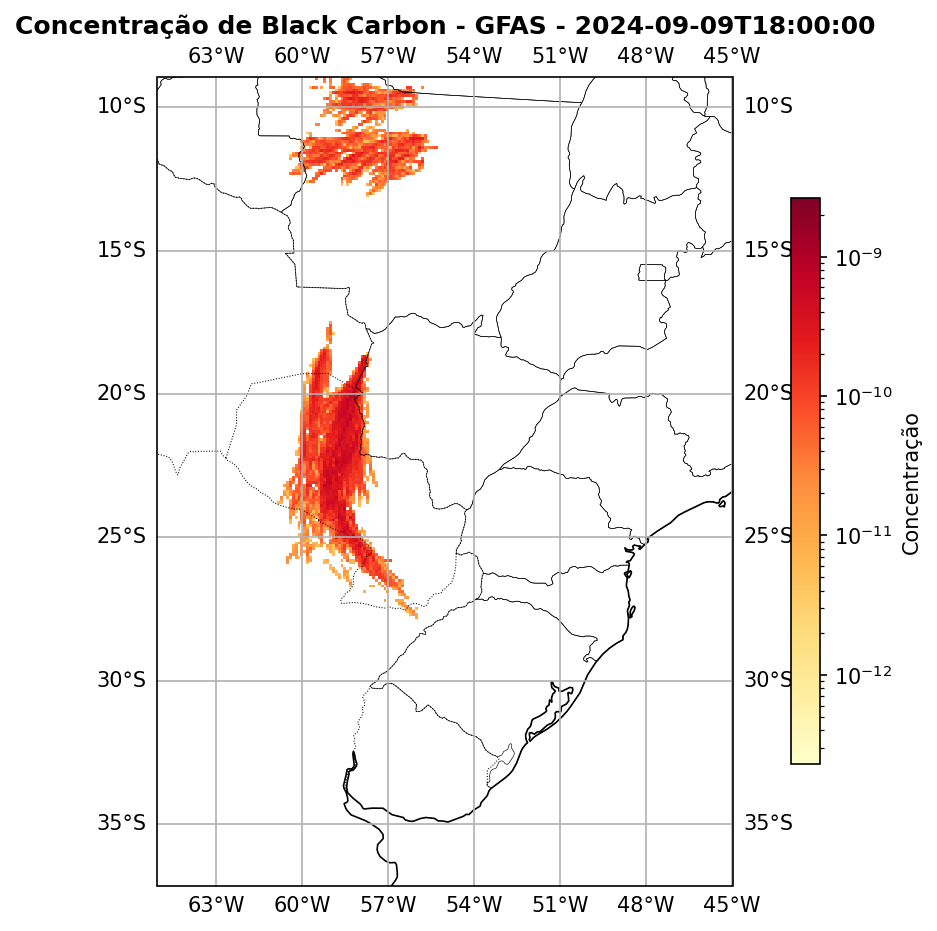
\includegraphics[width=\textwidth, trim=0cm 0cm 0cm 0.7cm, clip]{images/bc_003.png}
		\caption{2024-09-09 00:18:00}
		\label{fig:img13}
	\end{subfigure}	
	\hfill
	\begin{subfigure}[b]{0.31\textwidth}
		\centering
		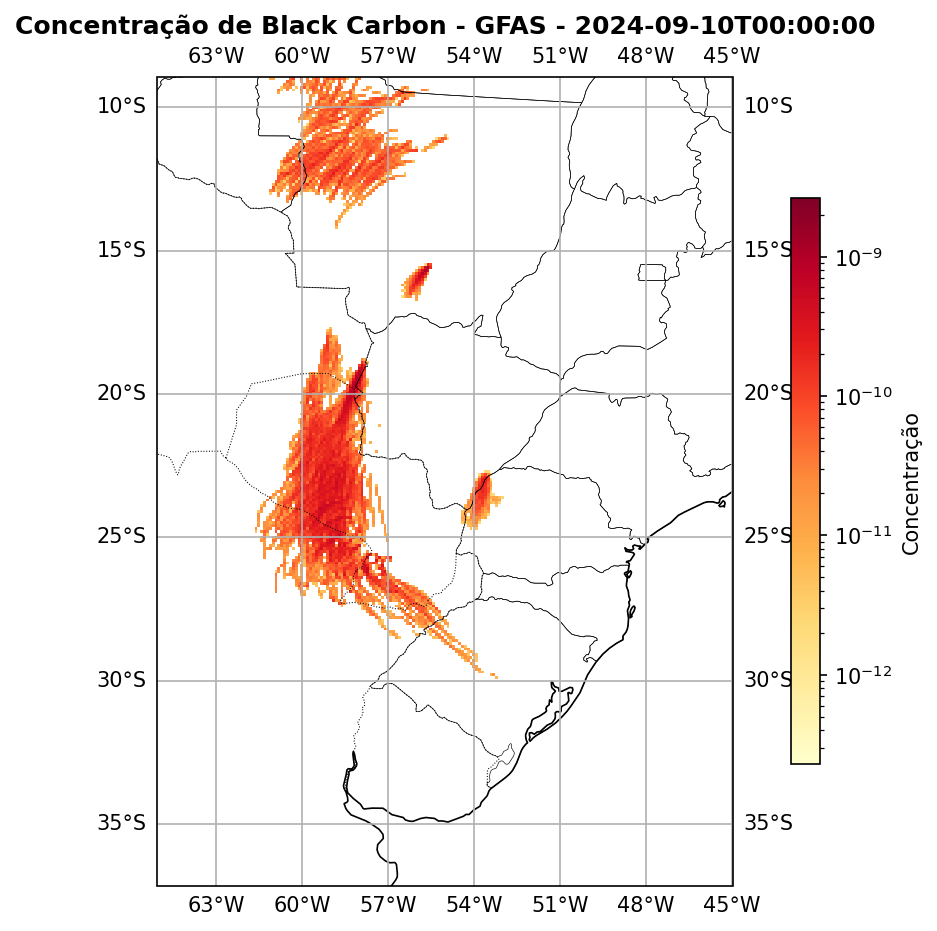
\includegraphics[width=\textwidth, trim=0cm 0cm 0cm 0.7cm, clip]{images/bc_004.png}
		\caption{2024-09-10 00:00:00}
		\label{fig:img14}
	\end{subfigure}	
	\hfill
	\begin{subfigure}[b]{0.31\textwidth}
		\centering
		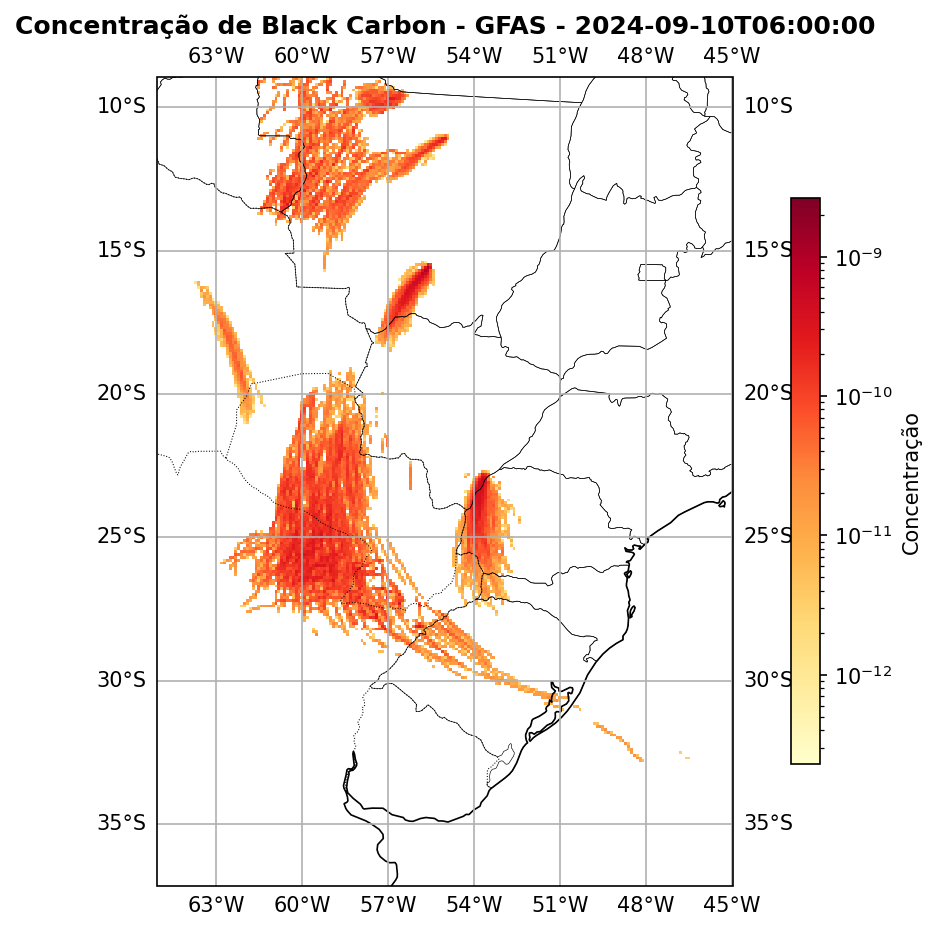
\includegraphics[width=\textwidth, trim=0cm 0cm 0cm 0.7cm, clip]{images/bc_005.png}
		\caption{2024-09-10 00:06:00}
		\label{fig:img15}
	\end{subfigure}	
	\hfill

	\vspace{0.8em} % Espaçamento vertical entre as linhas
	
	\begin{subfigure}[b]{0.31\textwidth}
		\centering
		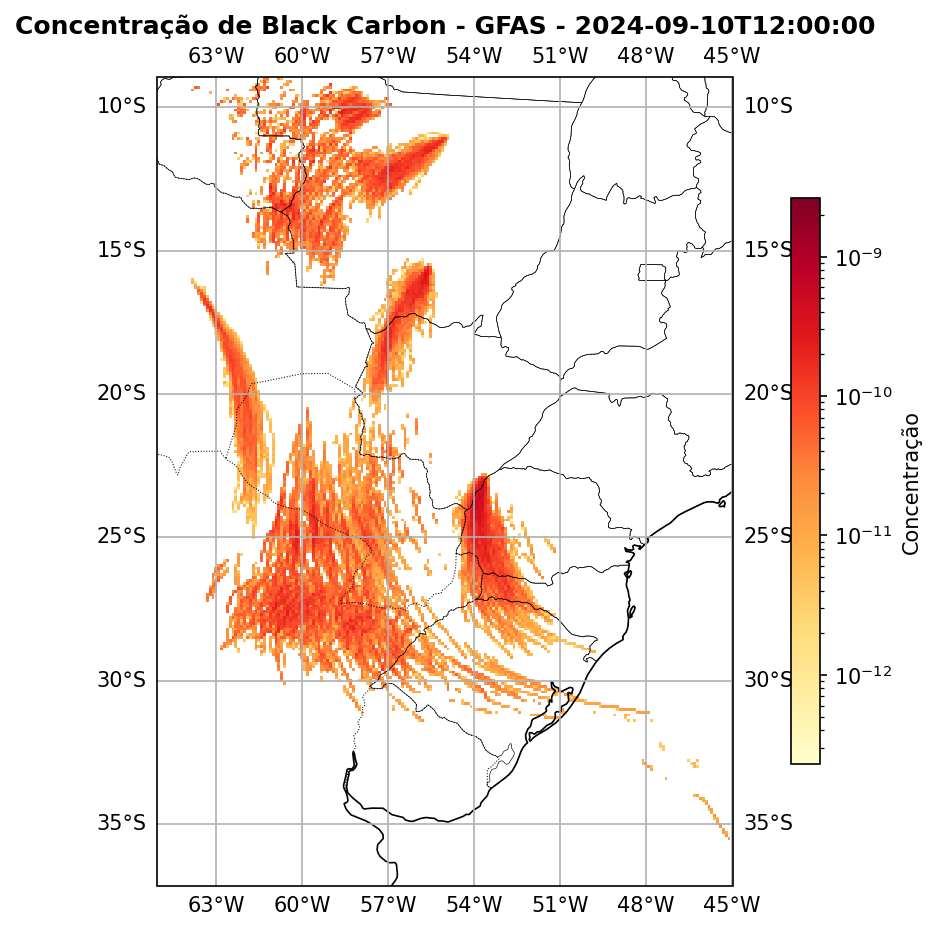
\includegraphics[width=\textwidth, trim=0cm 0cm 0cm 0.7cm, clip]{images/bc_006.png}
		\caption{2024-09-10 00:12:00}
		\label{fig:img16}
	\end{subfigure}	
	\hfill
	\begin{subfigure}[b]{0.31\textwidth}
		\centering
		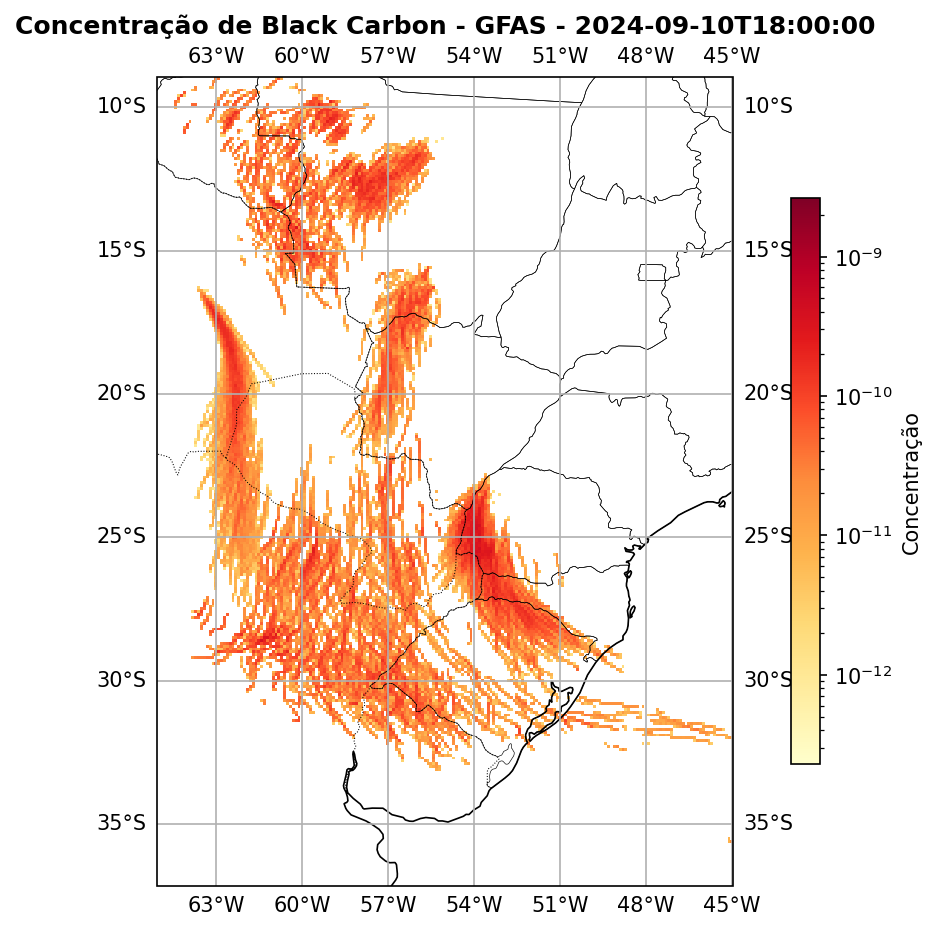
\includegraphics[width=\textwidth, trim=0cm 0cm 0cm 0.7cm, clip]{images/bc_007.png}
		\caption{2024-09-10 00:18:00}
		\label{fig:img17}
	\end{subfigure}	
	\hfill
	\begin{subfigure}[b]{0.31\textwidth}
		\centering
		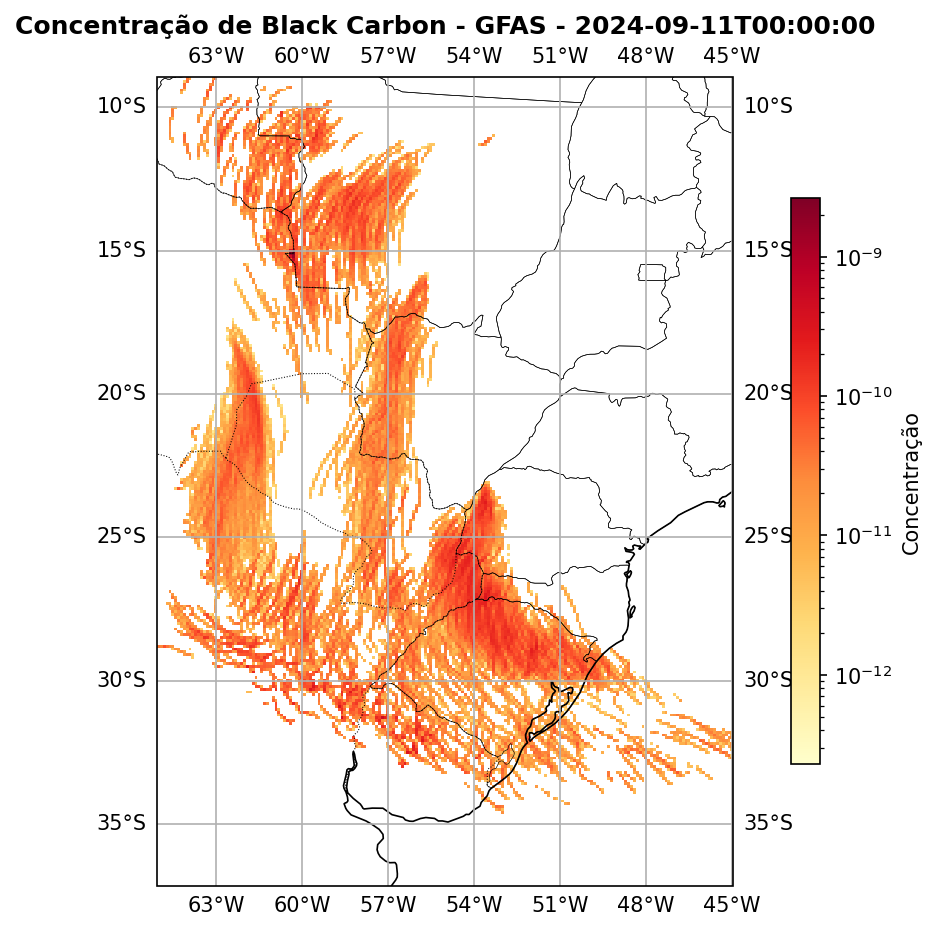
\includegraphics[width=\textwidth, trim=0cm 0cm 0cm 0.7cm, clip]{images/bc_008.png}
		\caption{2024-09-11 00:00:00}
		\label{fig:img18}
	\end{subfigure}	
	\hfill
	
	\vspace{0.8em} % Espaçamento vertical entre as linhas

	\begin{subfigure}[b]{0.31\textwidth}
		\centering
		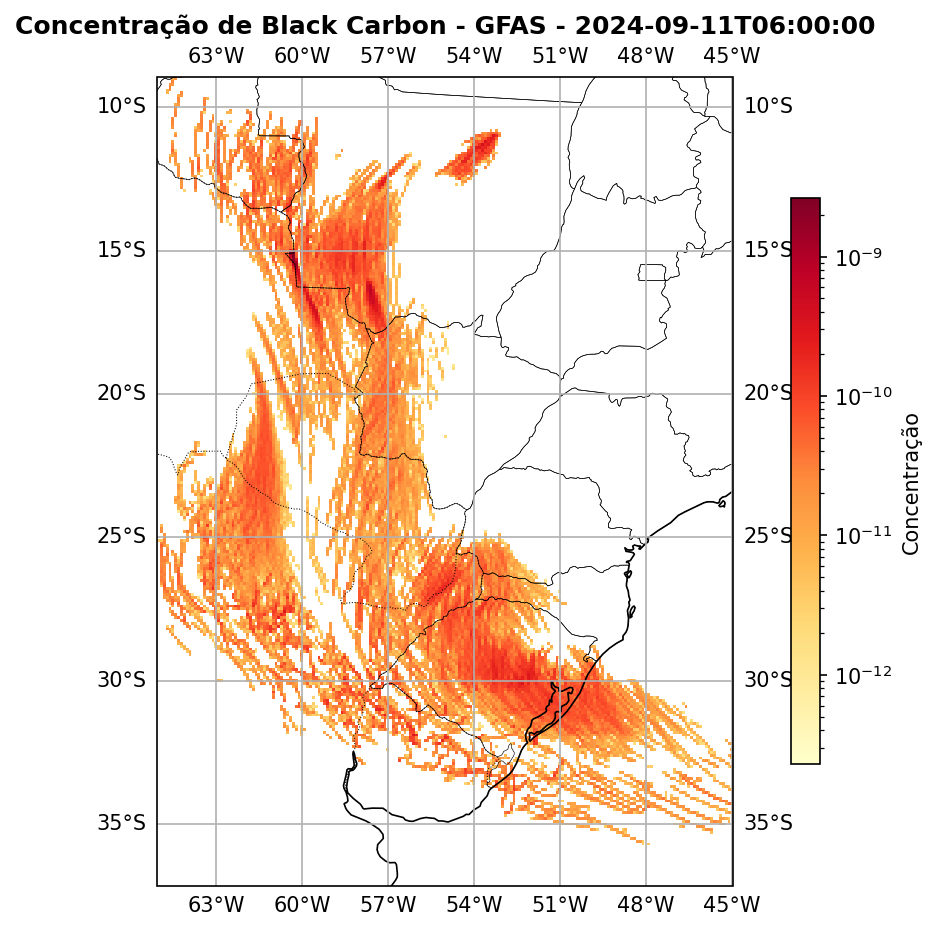
\includegraphics[width=\textwidth, trim=0cm 0cm 0cm 0.7cm, clip]{images/bc_009.png}
		\caption{2024-09-11 00:06:00}
		\label{fig:img19}
	\end{subfigure}	
	\hfill
	\begin{subfigure}[b]{0.31\textwidth}
		\centering
		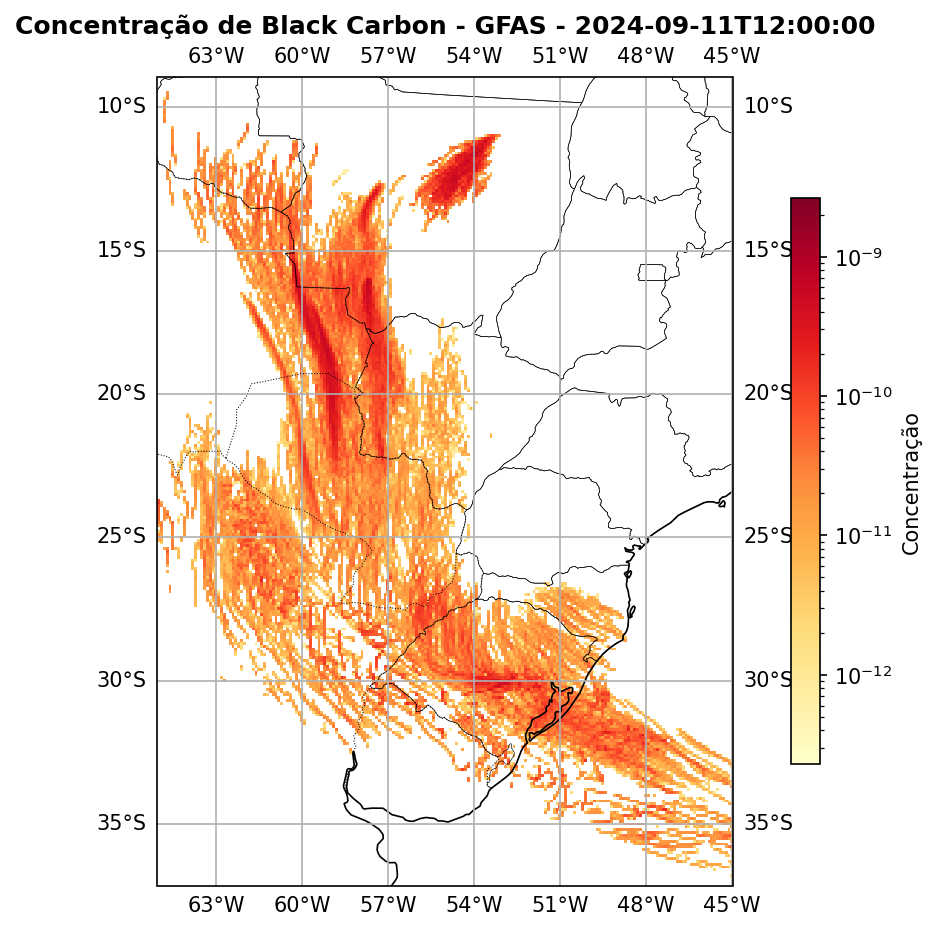
\includegraphics[width=\textwidth, trim=0cm 0cm 0cm 0.7cm, clip]{images/bc_010.png}
		\caption{2024-09-11 00:12:00}
		\label{fig:img20}
	\end{subfigure}	
	\hfill
	\begin{subfigure}[b]{0.31\textwidth}
		\centering
		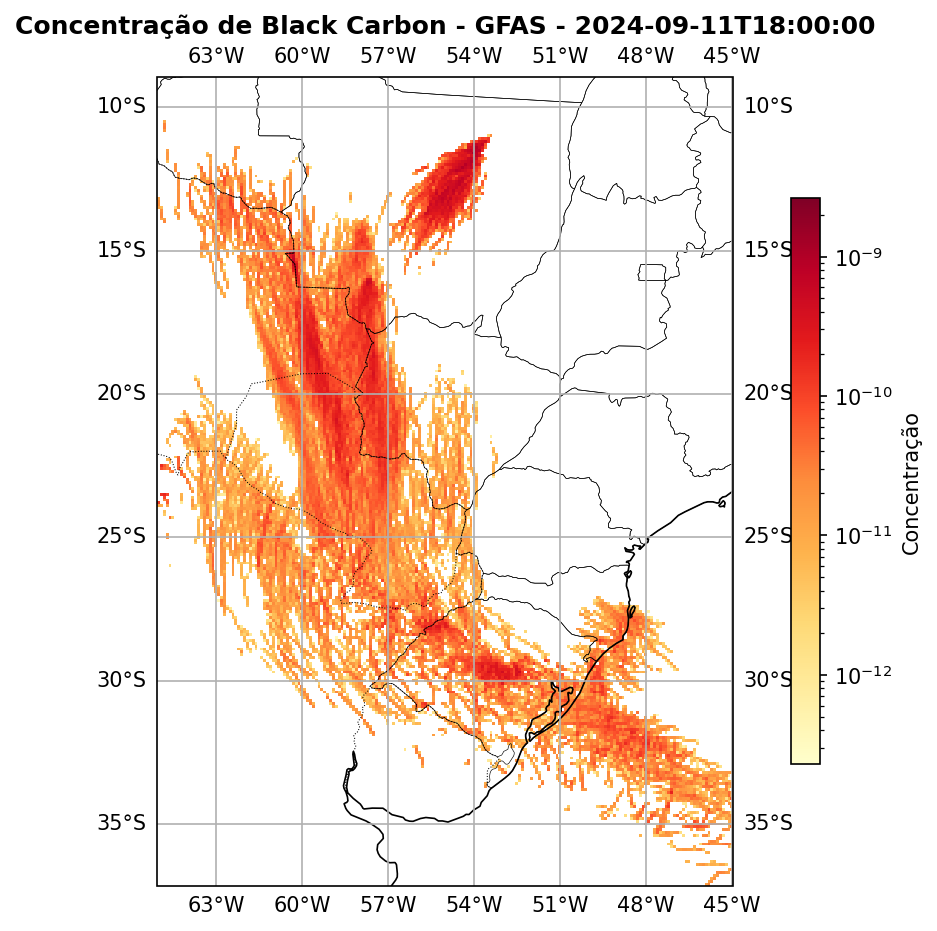
\includegraphics[width=\textwidth, trim=0cm 0cm 0cm 0.7cm, clip]{images/bc_011.png}
		\caption{2024-09-11 00:18:00}
		\label{fig:img21}
	\end{subfigure}
	\caption{Dispersão de black carbon simulada com o modelo HYSPLIT utilizando dados das reanálises ERA5 e GFAS.}
\end{figure}

\begin{figure}[htbp]
	\ContinuedFloat % Mantém a mesma numeração da figura anterior
	\centering
	
	% LINHA 5
	\begin{subfigure}[b]{0.31\textwidth}
		\centering
		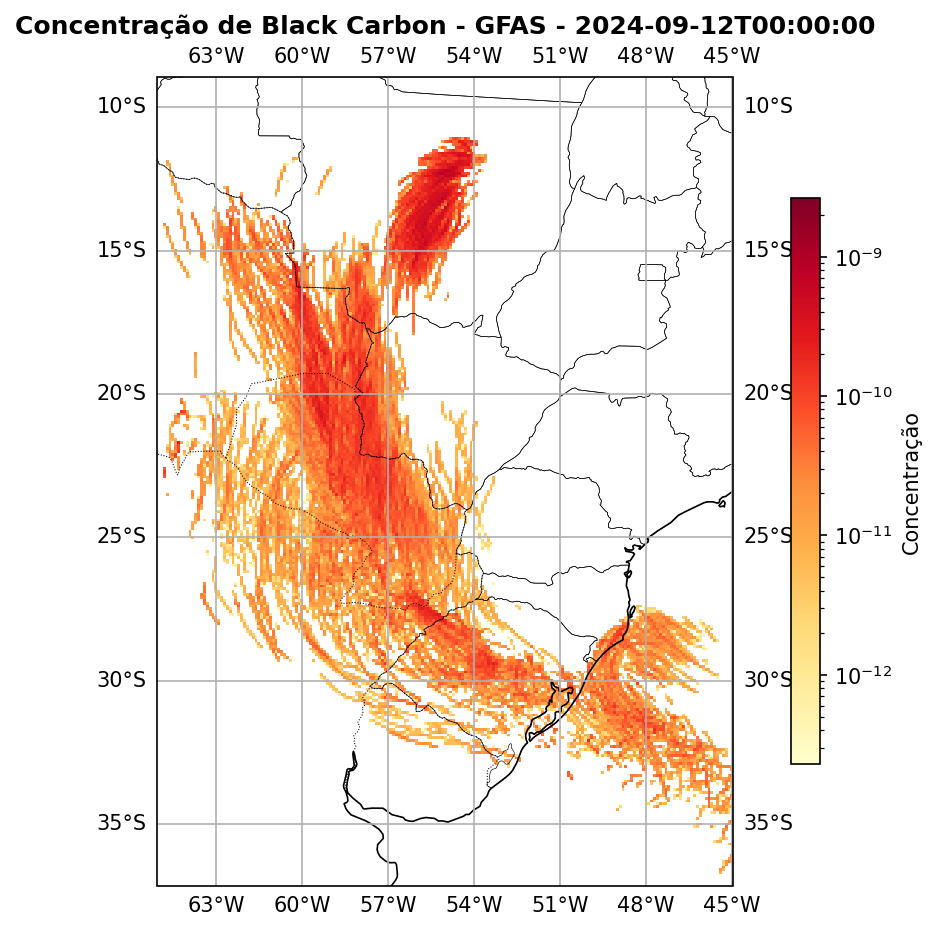
\includegraphics[width=\textwidth, trim=0cm 0cm 0cm 0.7cm, clip]{images/bc_012.png}
		\caption{2024-09-12 00:00:00}
		\label{fig:img22}
	\end{subfigure}    
	\hfill
	\begin{subfigure}[b]{0.31\textwidth}
		\centering
		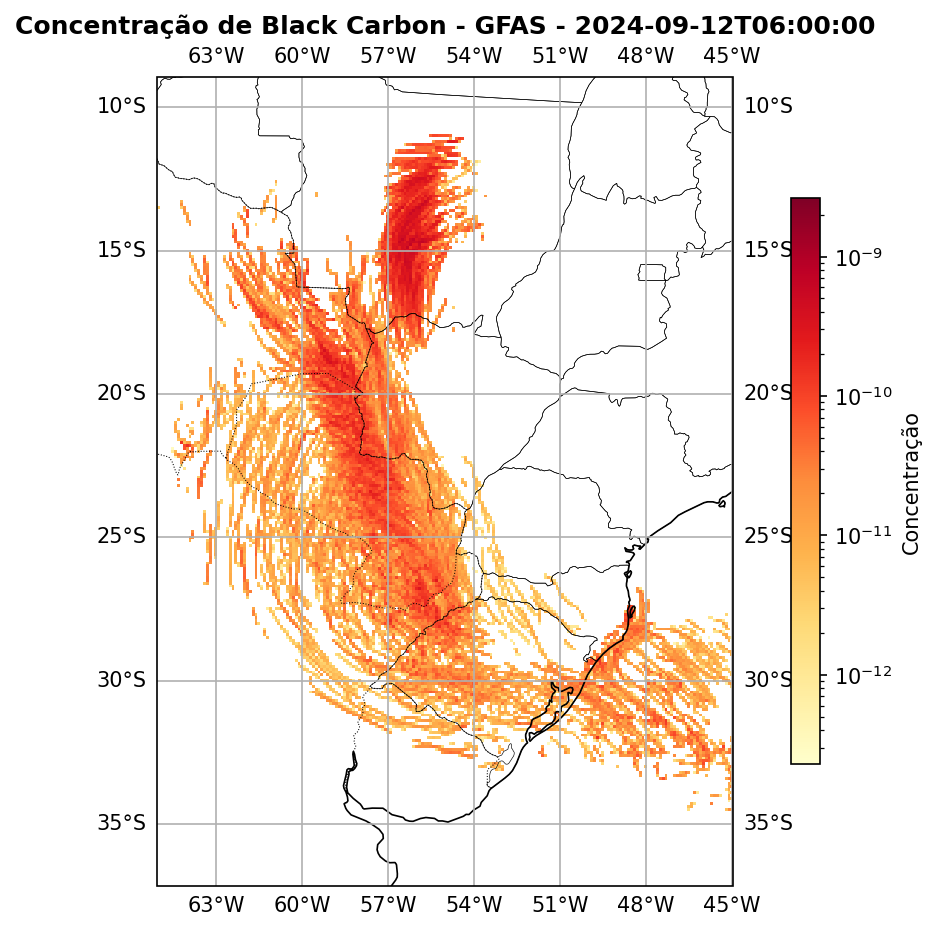
\includegraphics[width=\textwidth, trim=0cm 0cm 0cm 0.7cm, clip]{images/bc_013.png}
		\caption{2024-09-12 00:06:00}
		\label{fig:img23}
	\end{subfigure}    
	\hfill
	\begin{subfigure}[b]{0.31\textwidth}
		\centering
		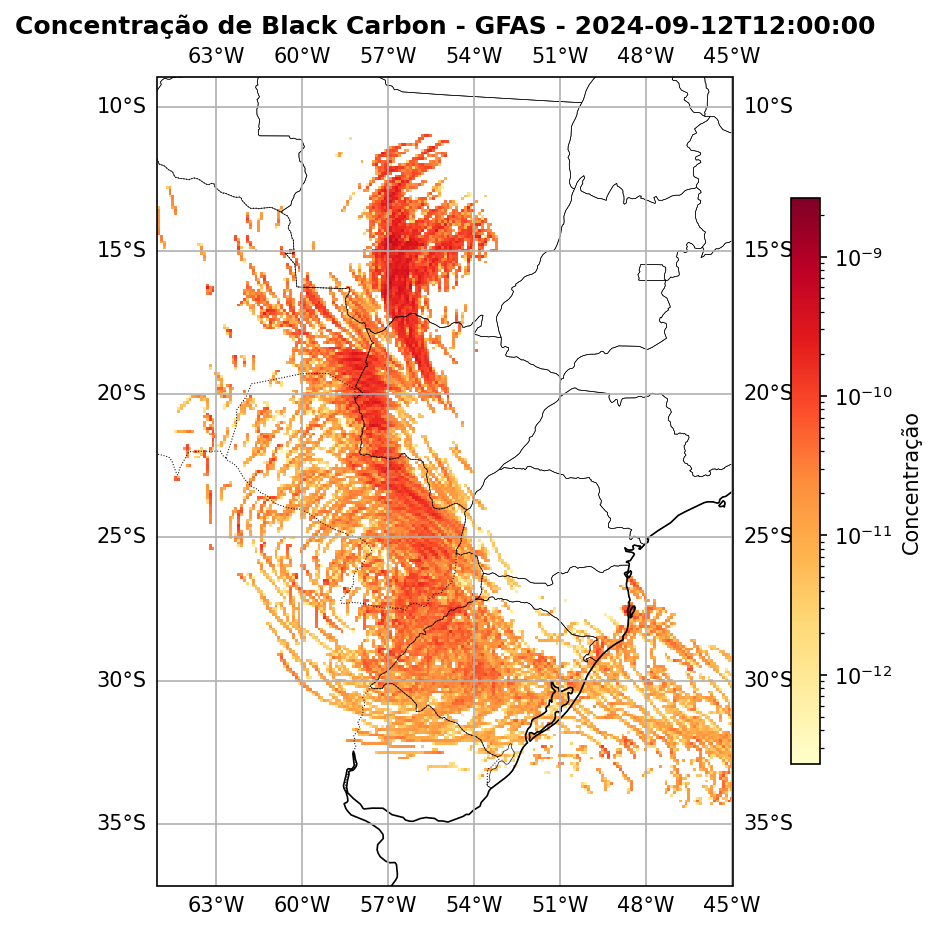
\includegraphics[width=\textwidth, trim=0cm 0cm 0cm 0.7cm, clip]{images/bc_014.png}
		\caption{2024-09-12 00:12:00}
		\label{fig:img24}
	\end{subfigure}    
	
	\vspace{0.8em}
	
	% LINHA 6
	\begin{subfigure}[b]{0.31\textwidth}
		\centering
		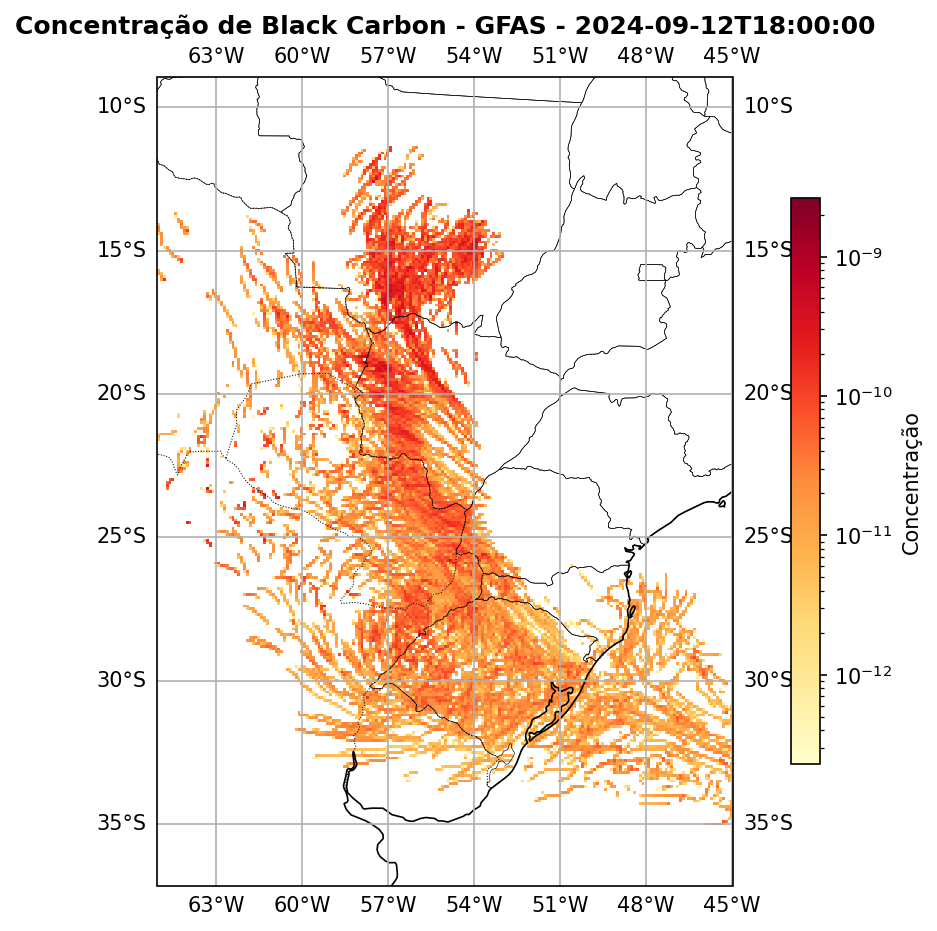
\includegraphics[width=\textwidth, trim=0cm 0cm 0cm 0.7cm, clip]{images/bc_015.png}
		\caption{2024-09-12 00:18:00}
		\label{fig:img25}
	\end{subfigure}
	
		\caption{Dispersão de black carbon simulada com o modelo HYSPLIT utilizando dados das reanálises ERA5 e GFAS. (continuação).} % Opcional
\end{figure}



\begin{figure}[htbp]
	\centering
	% --- LINHA 1 ---
	\begin{subfigure}[b]{0.31\textwidth}
		\centering
		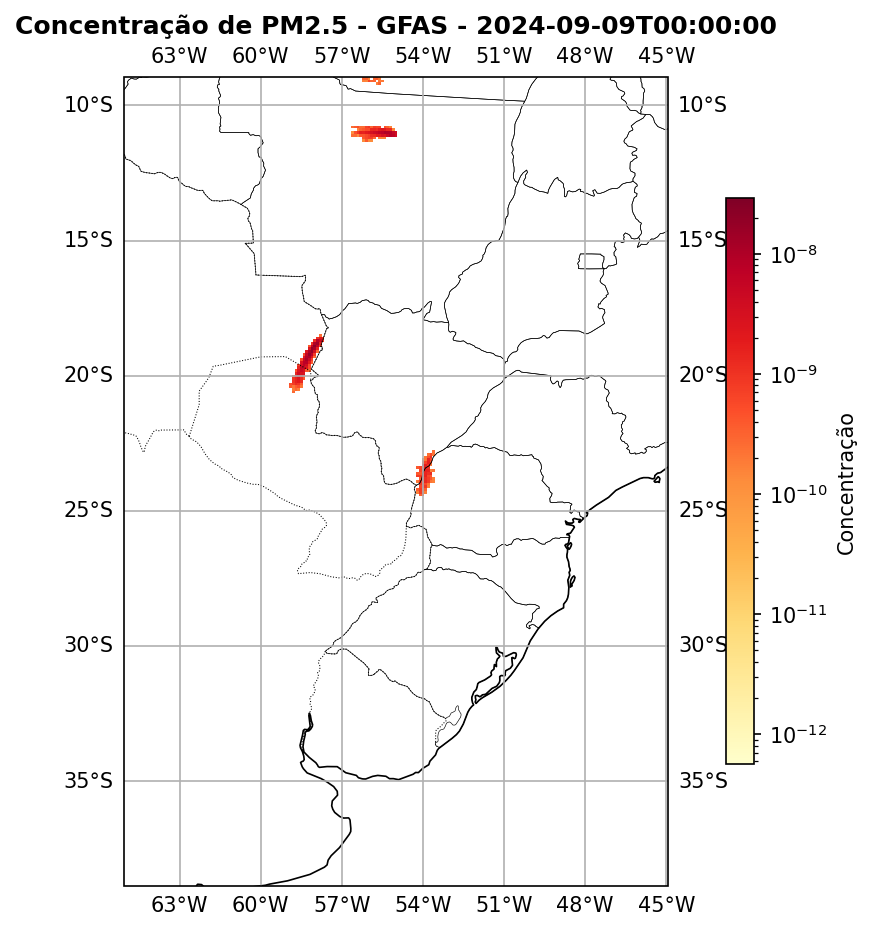
\includegraphics[width=\textwidth, trim=0cm 0cm 0cm 0.7cm, clip]{images/pm25_000.png}
		\caption{2024-09-09 00:00:00}
		\label{fig:img26}
	\end{subfigure}
	\hfill
	\begin{subfigure}[b]{0.31\textwidth}
		\centering
		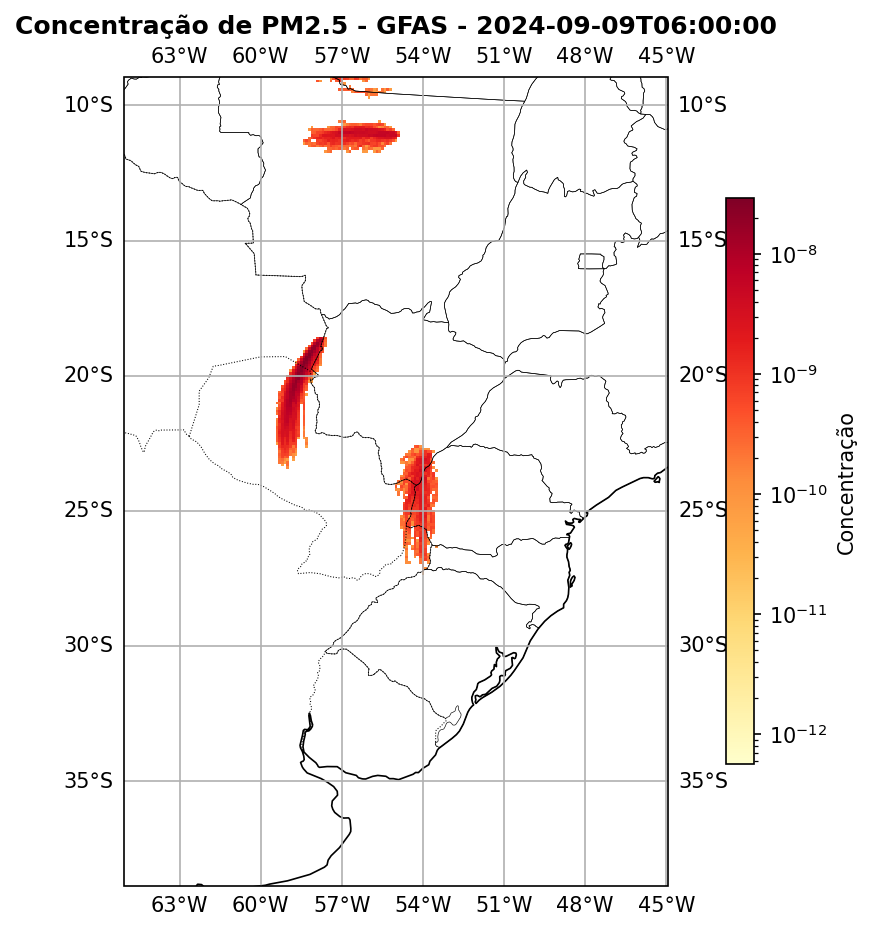
\includegraphics[width=\textwidth, trim=0cm 0cm 0cm 0.7cm, clip]{images/pm25_001.png}
		\caption{2024-09-09 00:06:00}
		\label{fig:img27}
	\end{subfigure}
	\hfill
	\begin{subfigure}[b]{0.31\textwidth}
		\centering
		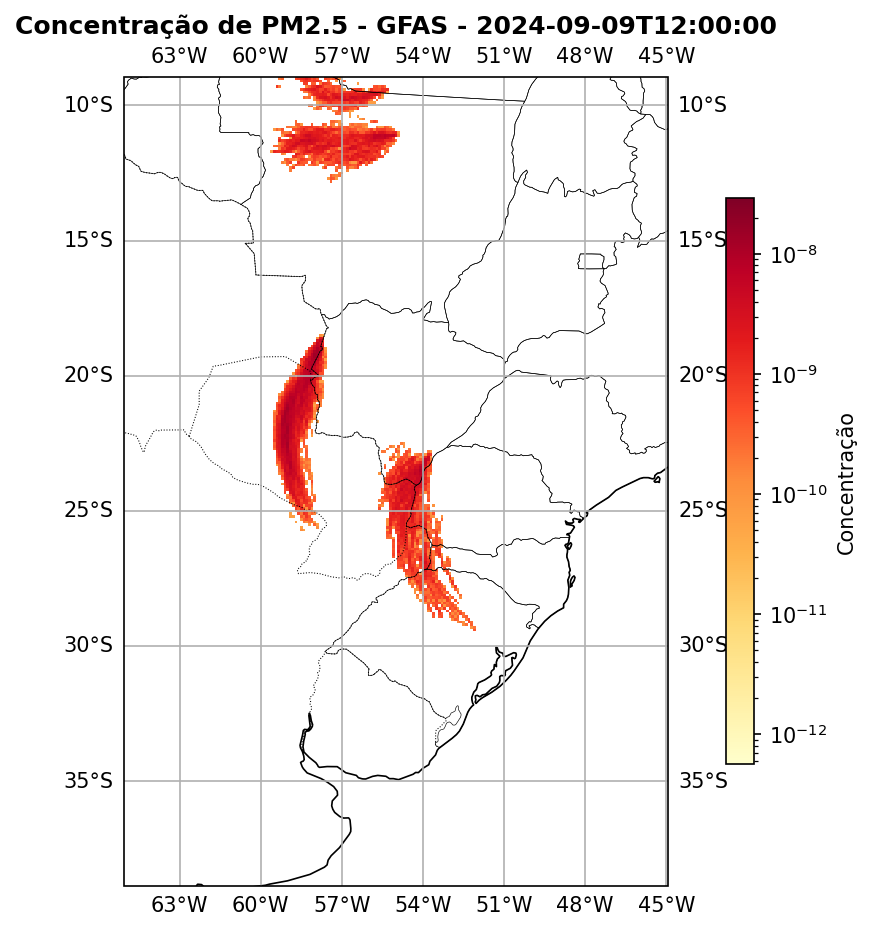
\includegraphics[width=\textwidth, trim=0cm 0cm 0cm 0.7cm, clip]{images/pm25_002.png}
		\caption{2024-09-09 00:12:00}
		\label{fig:img28}
	\end{subfigure}
	\hfill
	
	\vspace{0.8em} % Espaçamento vertical entre as linhas
	
	\begin{subfigure}[b]{0.31\textwidth}
		\centering
		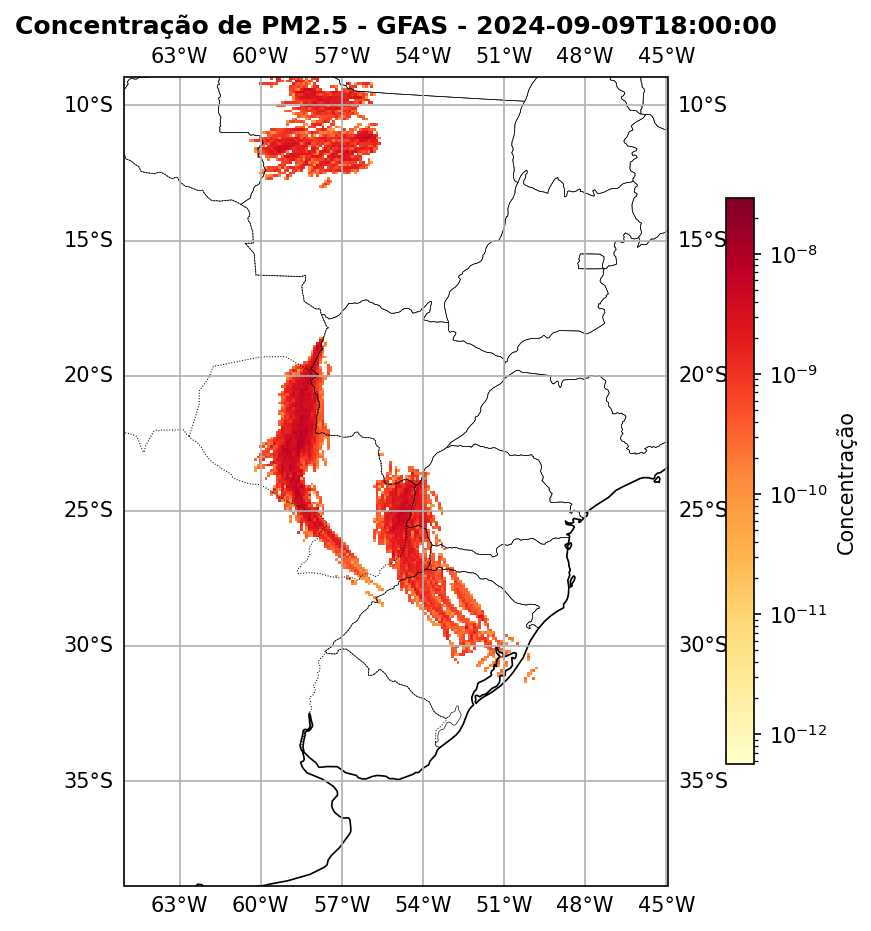
\includegraphics[width=\textwidth, trim=0cm 0cm 0cm 0.7cm, clip]{images/pm25_003.png}
		\caption{2024-09-09 00:18:00}
		\label{fig:img29}
	\end{subfigure}	
	\hfill
	\begin{subfigure}[b]{0.31\textwidth}
		\centering
		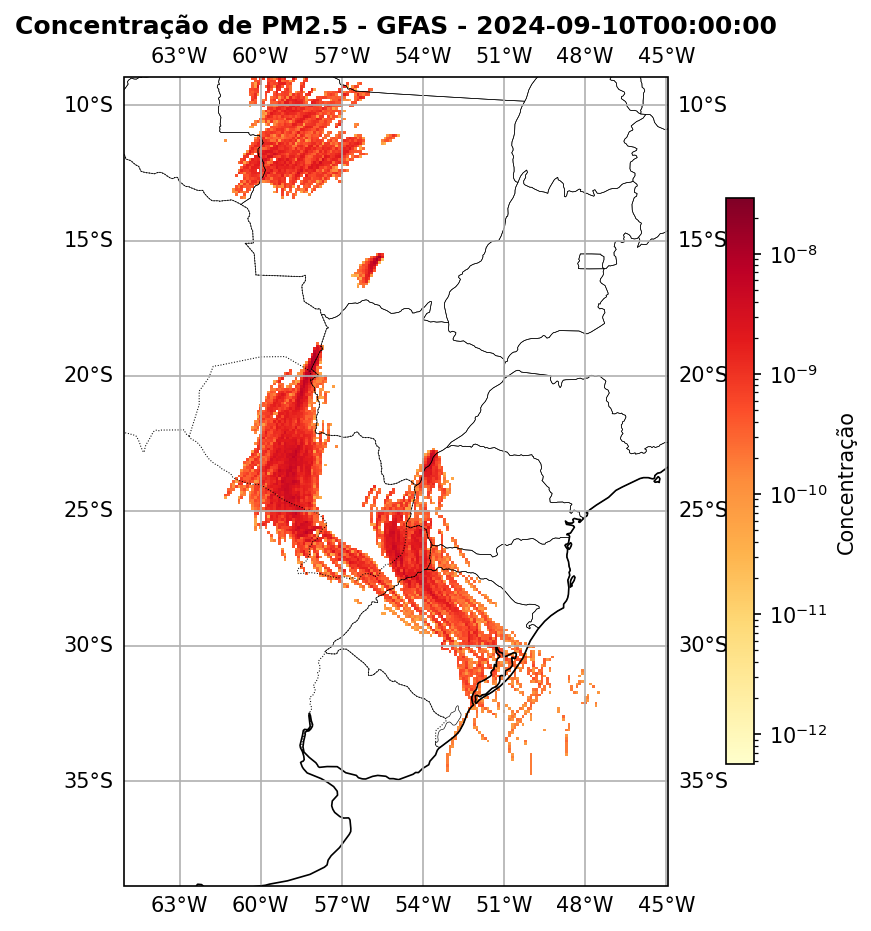
\includegraphics[width=\textwidth, trim=0cm 0cm 0cm 0.7cm, clip]{images/pm25_004.png}
		\caption{2024-09-10 00:00:00}
		\label{fig:img30}
	\end{subfigure}	
	\hfill
	\begin{subfigure}[b]{0.31\textwidth}
		\centering
		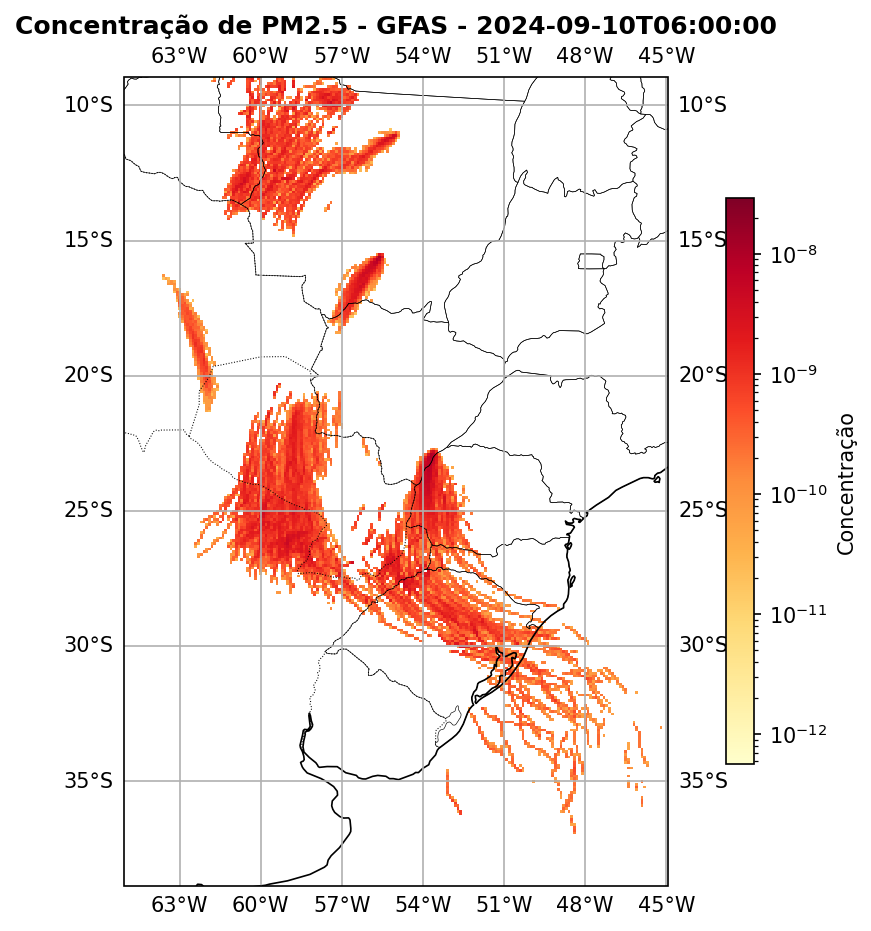
\includegraphics[width=\textwidth, trim=0cm 0cm 0cm 0.7cm, clip]{images/pm25_005.png}
		\caption{2024-09-10 00:06:00}
		\label{fig:img31}
	\end{subfigure}	
	\hfill
	
	\vspace{0.8em} % Espaçamento vertical entre as linhas
	
	\begin{subfigure}[b]{0.31\textwidth}
		\centering
		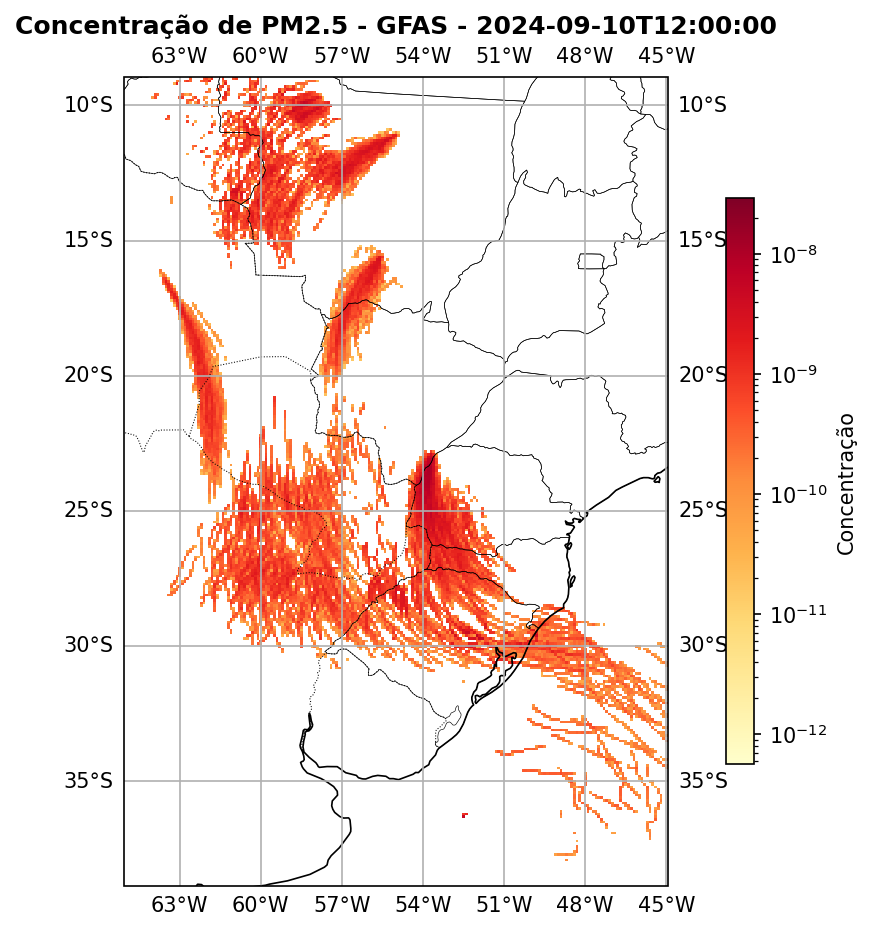
\includegraphics[width=\textwidth, trim=0cm 0cm 0cm 0.7cm, clip]{images/pm25_006.png}
		\caption{2024-09-10 00:12:00}
		\label{fig:img32}
	\end{subfigure}	
	\hfill
	\begin{subfigure}[b]{0.31\textwidth}
		\centering
		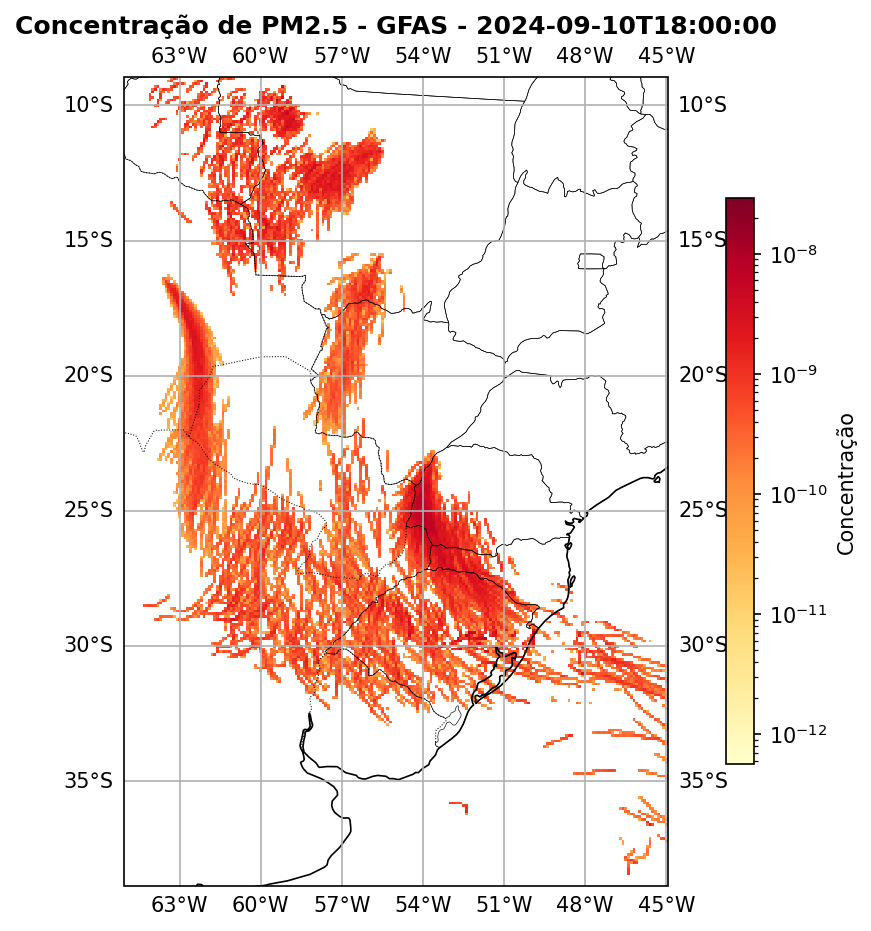
\includegraphics[width=\textwidth, trim=0cm 0cm 0cm 0.7cm, clip]{images/pm25_007.png}
		\caption{2024-09-10 00:18:00}
		\label{fig:img33}
	\end{subfigure}	
	\hfill
	\begin{subfigure}[b]{0.31\textwidth}
		\centering
		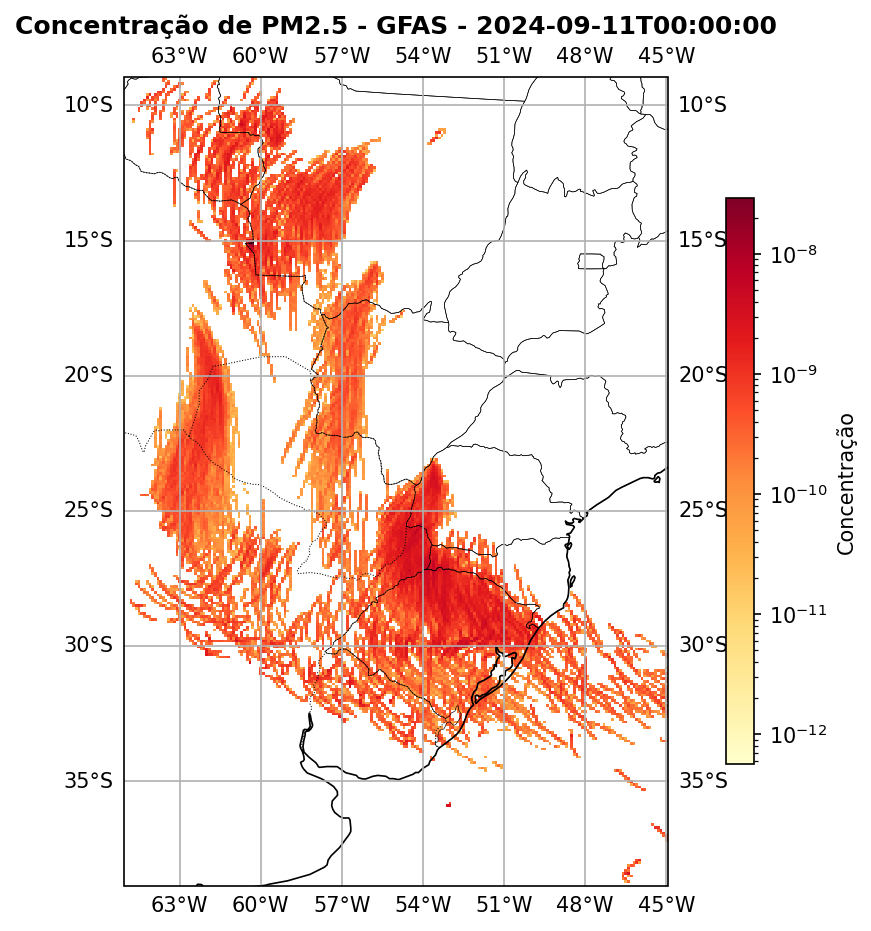
\includegraphics[width=\textwidth, trim=0cm 0cm 0cm 0.7cm, clip]{images/pm25_008.png}
		\caption{2024-09-11 00:00:00}
		\label{fig:img34}
	\end{subfigure}	
	\hfill
	
	\vspace{0.8em} % Espaçamento vertical entre as linhas
	
	\begin{subfigure}[b]{0.31\textwidth}
		\centering
		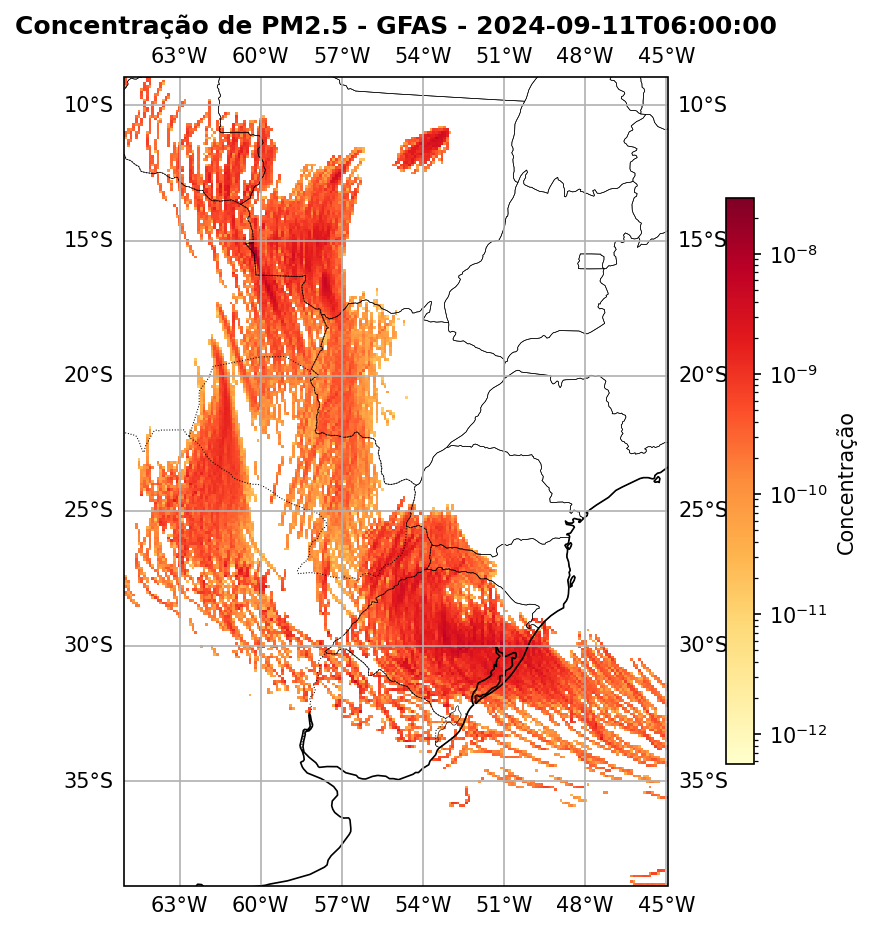
\includegraphics[width=\textwidth, trim=0cm 0cm 0cm 0.7cm, clip]{images/pm25_009.png}
		\caption{2024-09-11 00:06:00}
		\label{fig:img35}
	\end{subfigure}	
	\hfill
	\begin{subfigure}[b]{0.31\textwidth}
		\centering
		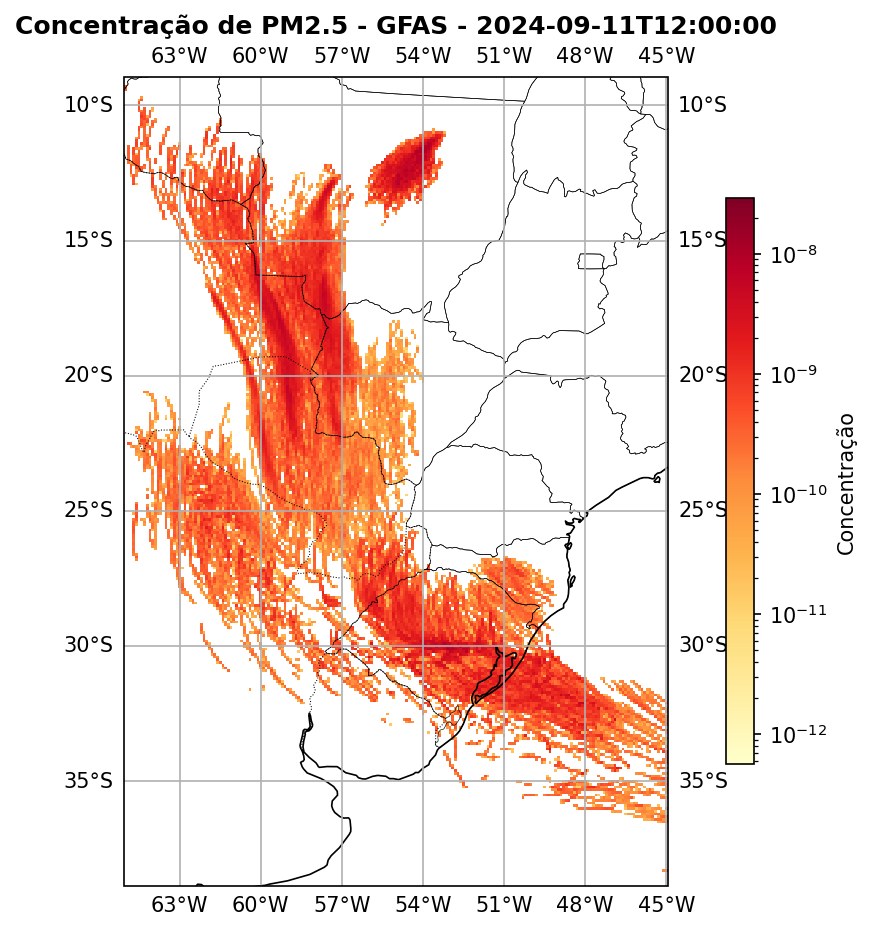
\includegraphics[width=\textwidth, trim=0cm 0cm 0cm 0.7cm, clip]{images/pm25_010.png}
		\caption{2024-09-11 00:12:00}
		\label{fig:img36}
	\end{subfigure}	
	\hfill
	\begin{subfigure}[b]{0.31\textwidth}
		\centering
		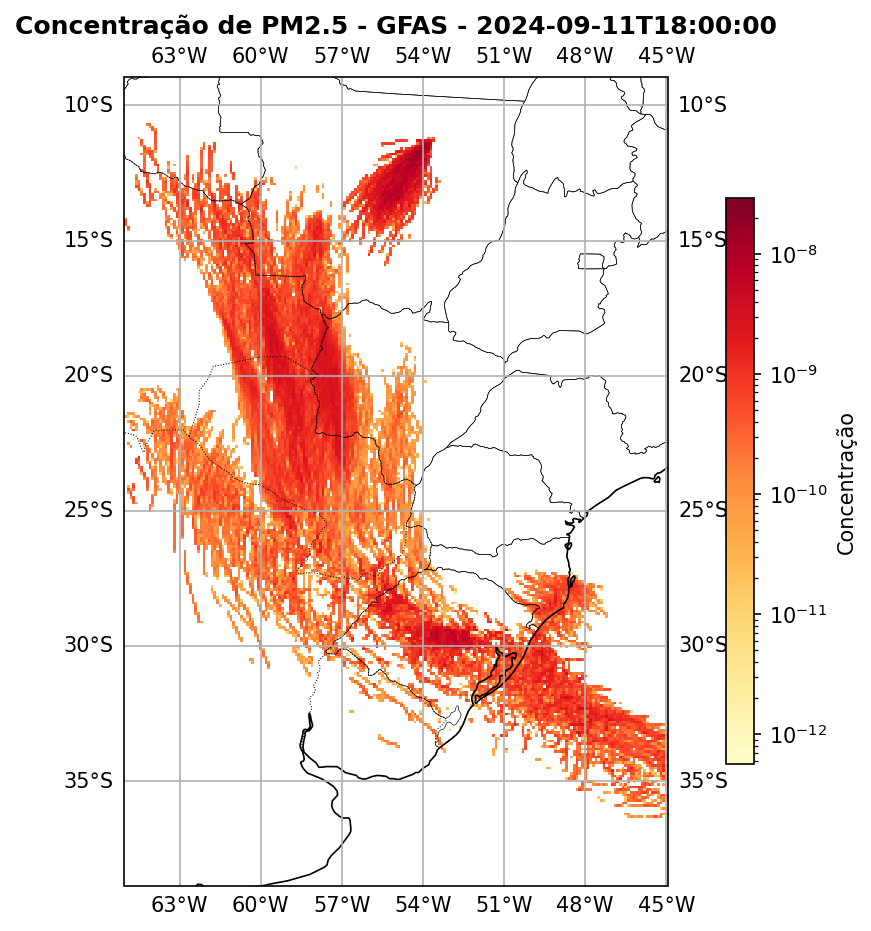
\includegraphics[width=\textwidth, trim=0cm 0cm 0cm 0.7cm, clip]{images/pm25_011.png}
		\caption{2024-09-11 00:18:00}
		\label{fig:img37}
	\end{subfigure}
	\caption{Dispersão de PM2.5 simulada com o modelo HYSPLIT utilizando dados das reanálises ERA5 e GFAS.}
\end{figure}

\begin{figure}[htbp]
	\ContinuedFloat % Mantém a mesma numeração da figura anterior
	\centering
	
	% LINHA 5
	\begin{subfigure}[b]{0.31\textwidth}
		\centering
		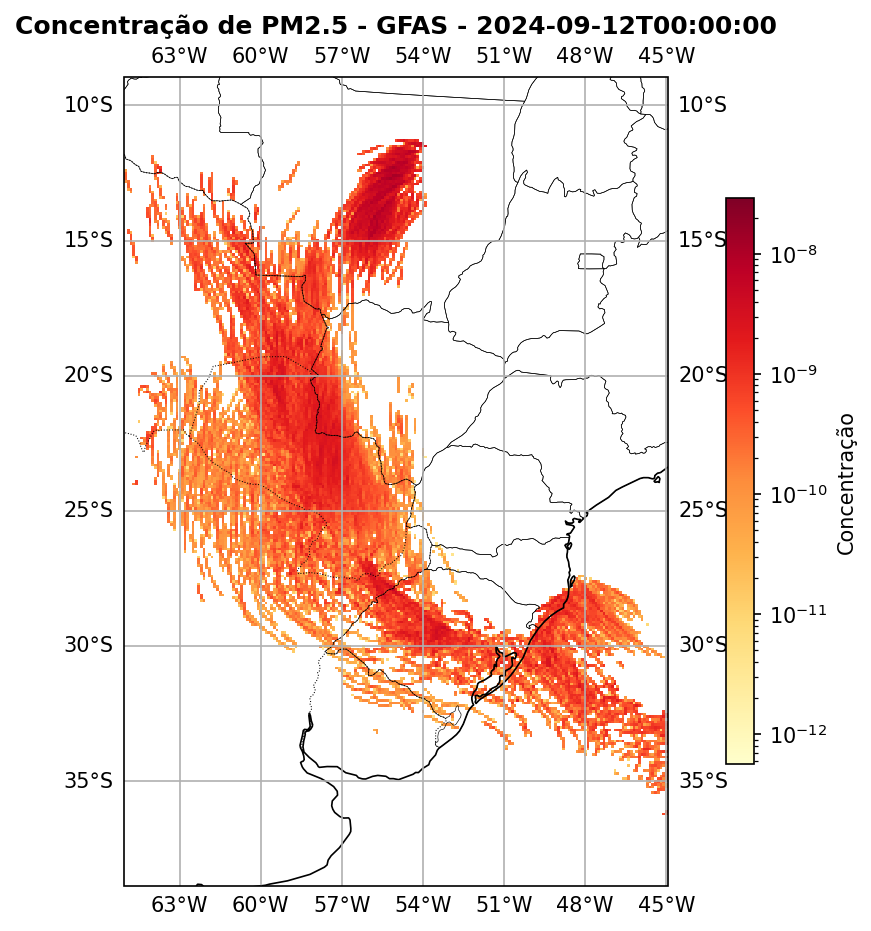
\includegraphics[width=\textwidth, trim=0cm 0cm 0cm 0.7cm, clip]{images/pm25_012.png}
		\caption{2024-09-12 00:00:00}
		\label{fig:img38}
	\end{subfigure}    
	\hfill
	\begin{subfigure}[b]{0.31\textwidth}
		\centering
		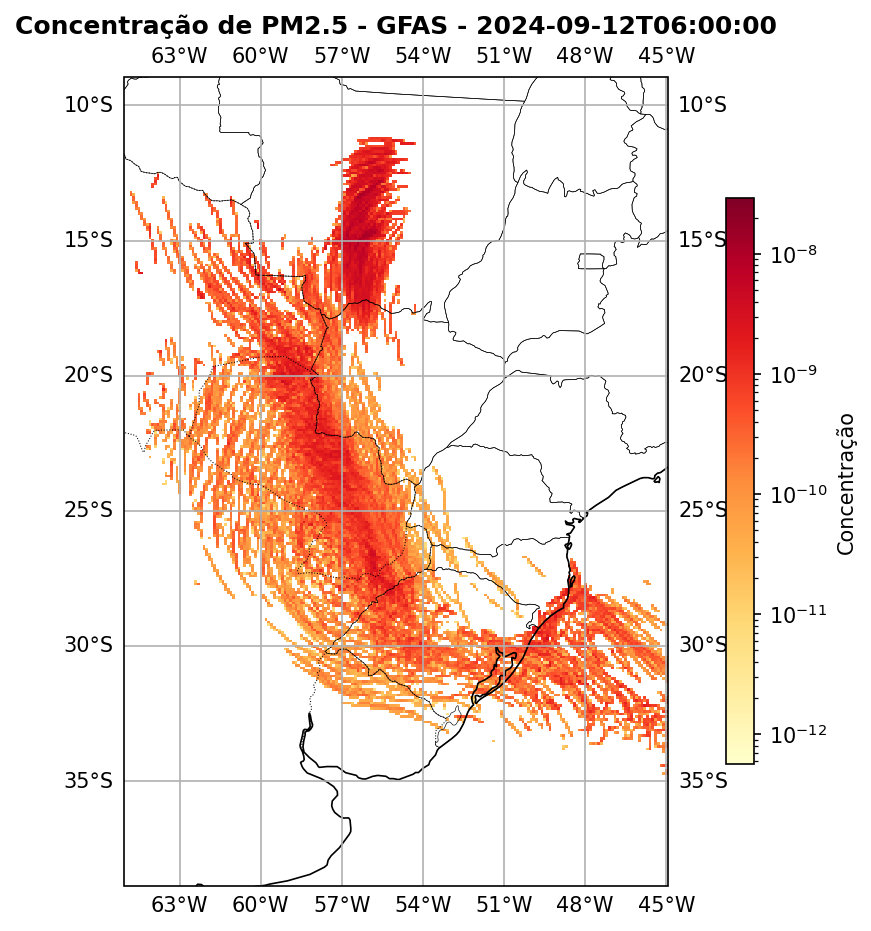
\includegraphics[width=\textwidth, trim=0cm 0cm 0cm 0.7cm, clip]{images/pm25_013.png}
		\caption{2024-09-12 00:06:00}
		\label{fig:img39}
	\end{subfigure}    
	\hfill
	\begin{subfigure}[b]{0.31\textwidth}
		\centering
		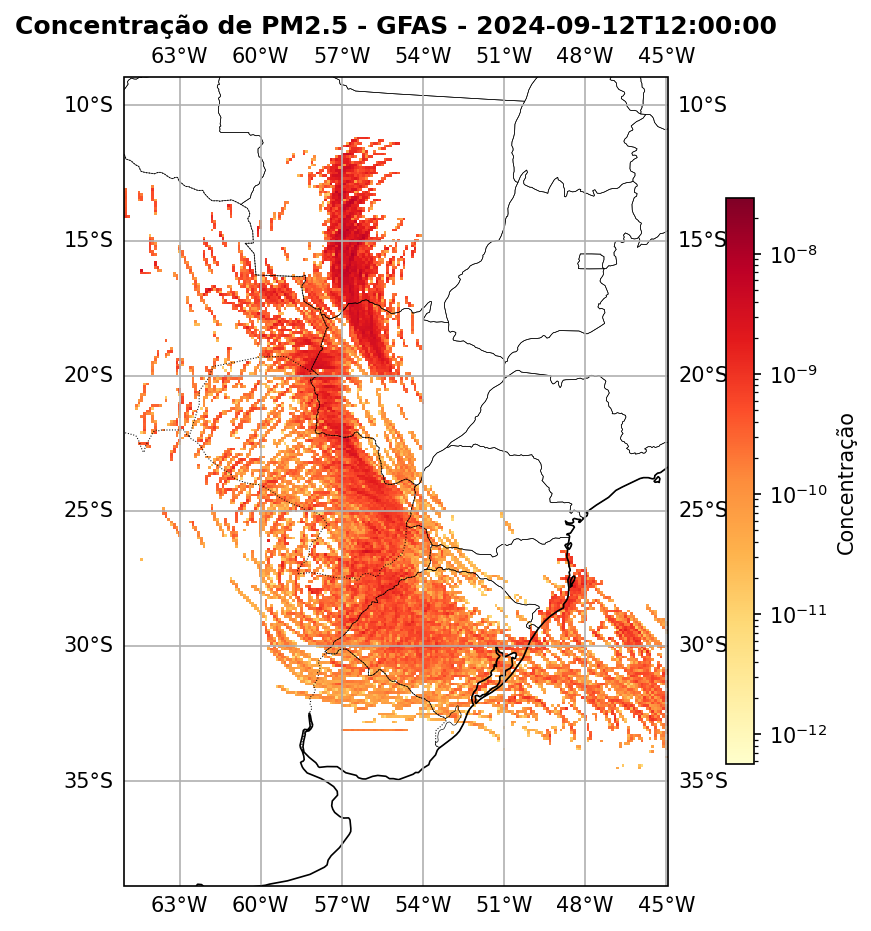
\includegraphics[width=\textwidth, trim=0cm 0cm 0cm 0.7cm, clip]{images/pm25_014.png}
		\caption{2024-09-12 00:12:00}
		\label{fig:img40}
	\end{subfigure}    
	
	\vspace{0.8em}
	
	% LINHA 6
	\begin{subfigure}[b]{0.31\textwidth}
		\centering
		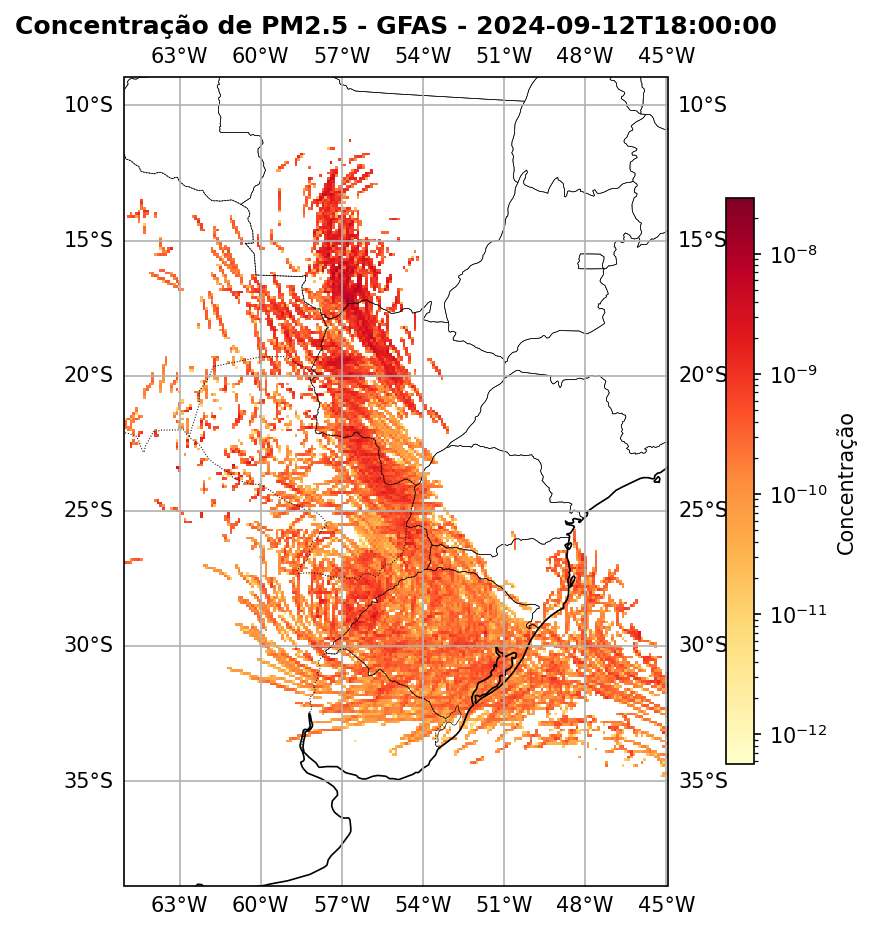
\includegraphics[width=\textwidth, trim=0cm 0cm 0cm 0.7cm, clip]{images/pm25_015.png}
		\caption{2024-09-12 00:18:00}
		\label{fig:img41}
	\end{subfigure}
	
	\caption{Dispersão de PM2.5 simulada com o modelo HYSPLIT utilizando dados das reanálises ERA5 e GFAS. (continuação).} % Opcional
\end{figure}




	
	% ----------------------------------------------------------
	% ELEMENTOS PÓS-TEXTUAIS
	% ----------------------------------------------------------
	\postextual
	
	% Referências bibliográficas
	\begingroup
	\SingleSpacing
	\printbibliography[title=REFERÊNCIAS]
	\endgroup
	
	% Apêndices
	%\begin{apendicesenv}
	%	\input{aftertext/apendice_a}
	%\end{apendicesenv}
	
	% Anexos
	%\begin{anexosenv}
	%	\input{aftertext/anexo_a}
	%\end{anexosenv}
	
\end{document}
